\chapter{Time Series}
\section{Components of Time Series}
Whether we wish to predict the trend in financial markets or electricity consumption, time is an important factor that must now be considered in our models. For example, it would be crucial to not only know when the electricity demand will move up, but also when it will move down. When forecasting Time Series data, the aim is to estimate how the sequence of observations will continue into the future. The simplest Time Series forecasting methods use only information on the variable to be forecast, and make no attempt to discover the factors that affect its behaviour. Therefore they will extrapolate trend and seasonal patterns, but they ignore all other information such as marketing initiatives, competitor activity, changes in economic conditions, and so on. 
\par Time-Series is a sequential set of observations(data points), usually recorded in a proper chronological order and is mathematically formulated as a set of vectors$$ x(t),t = 0,1,2,... $$ where t denotes the elapsed time. A Time Series containing records of a single variable is termed as univariate, otherwise when records of more than one variable are considered, it is termed as multivariate. Furthermore, Time-Series can be continuous or discrete \cite{chatfield2003analysis}. In a continuous Time Series observations are measured at every instance of time, whereas a discrete Time Series contains observations measured at discrete points of
time. For instance temperature, load demand etc. can be presented as continuous Time-Series, whereas exchange rates between two currencies is considered to be under the class of discrete Time Series. Usually in a discrete Time-Series the consecutive observations are recorded at equally spaced time intervals such as hourly, daily, weekly, monthly or yearly time separations. The variable under study in a discrete Time-Series is supposed to be measured as a continuous variable using the real number scale.
Furthermore, concerning continuous Time-Series, they can be transformed to discrete by resampling (merging) observations over a specified time period.
\par A Time-Series is non-deterministic in nature, i.e. we cannot predict with certainty what will
occur in future. Generally a Time Series \textbf{{x(t),t = 0,1, 2,...}} is assumed to follow certain
probability model which describes the joint distribution of the random variable x. The formula that characterizes the probability structure of the Time-Series is termed as \textit{a
stochastic process} [23]. Thus the sequence of observations of the series is actually a sample
realization of the stochastic process that produced it.
A usual assumption is that the Time Series variables are independent and identically
distributed e.g they follow the normal distribution. However, an
interesting point is that Time Series are in fact following more or less some
regular pattern in long term. For example if the temperature today of a particular city is
extremely high, then it can be reasonably presumed that tomorrow’s temperature will also
likely to be high. This is the reason why Time Series forecasting using a proper technique,
yields result close to the actual value.
\par 
In general, a Time Series is simply a series of data points ordered in time. In a Time Series, time is often the independent variable and the goal is usually to make a forecast for the future, however, there are other aspects that come into play when dealing with Time Series.
\begin{itemize}
    \item \textbf{Is it stationary?} Stationarity is an important characteristic of Time Series. A Time Series is said to be stationary if its statistical properties do not change over time. In other words, it has constant mean and variance, and covariance is independent of time. Ideally, we want to have a stationary Time Series for modelling.
    \item \textbf{Is there a seasonality pattern?} Seasonality refers to periodic fluctuations. For instance, electricity load demand peaks during the day and presents lower values during the night.
    \item \textbf{Is the target variable autocorrelated?}
\end{itemize}
\par There are two main goals of Time Series analysis: \textbf {(a) identifying the nature of the phenomenon represented by the sequence of observations}, and \textbf{(b) forecasting (predicting future values of the Time Series variable)}. Both of these goals require that the pattern of observed Time Series data is identified and more or less formally described. Once the pattern is established, we can interpret and integrate it with other data. Regardless of the depth of our understanding and the validity of our interpretation of the phenomenon, we can extrapolate the identified pattern to predict future events. Most Time Series patterns can be described in terms of two basic classes of components: \textit{trend and seasonality} \cite{box2015time}. The term trend represents a general systematic linear or (most often) nonlinear component that changes over time and does not repeat or at least does not repeat within the time range captured by our data. The general tendency of a Time Series to increase, decrease or stagnate over a long period of
time is termed as Secular Trend or simply Trend. Thus, it can be said that trend is a long term
movement in a Time Series. 
\par The term seasonality may have a similar nature (e.g. a plateau followed by a period of exponential growth), however, it repeats itself in systematic intervals over time. More formally, it's defined as the correlational dependency of order k between the $i_{th}$  series' observation and the $(i-k)_{th}$ observation, known as autocorrelation; k is usually called the lag. If the measurement error is not too large, seasonality can be visually identified in the series as a pattern that repeats every k elements. Those two general classes of Time Series components may coexist in real-life data. Seasonal patterns of Time-Series can be represented by correlograms. A correlogram visualizes and quantifies the autocorrelation function (ACF), or in other words the sequential correlation coefficients (and their standard errors) for consecutive lags in a predefined range of lags. To determine a proper model for a given time series data, it is necessary to carry out the ACF and PACF analysis. These statistical measures reflect how the observations in a time series are related to each other. For modeling and forecasting purpose it is often useful to plot the ACF and PACF against consecutive time lags \cite{hyndman2018forecasting}. These plots help in determining the order of AR and MA terms. Below we give their mathematical definitions:
For a time series ${x(t),t=0,1,2,...}$ the Autocovariance at lag k is defined as:
$$\gamma_{k}=Cov(x_{t},x_{t+k})=E[(x_t-\mu)(x_{t+k}-\mu)]$$
 The Autocorrelation Coeffient at lag k is defined as: 
$$\rho_k=\frac{\gamma_k}{\gamma_o}$$
\par Here $\mu$  is the mean of the time series, i.e. $\mu=E[x_{t}]$. The Autocovariance at lag zero i.e. $\gamma_{o}$ is the variance of the time series. From the definition it is clear that the autocorrelation coefficient $\rho_k$ is dimensionless and so is independent of the scale of measurement. It's obvious that $-1\leq \rho_{k} \leq 1$. Box \& Jenkins termed $\gamma_{k}$ as the theoretical Autocovariance Function (ACVF) and $\rho_{k}$ as the theoretical Autocorrelation Function (ACF). Furthermore, Partial Autocorrelation fnction (PACF) represents the correlation between an observation k in the past and the current observation, after checking for observations at intermediate lags (i.e. at lags $<k$). In general, the stochastic process of a Time-Series is not known and thus it's not possible to determine neither the actual nor the theoretical ACF and PACF values. The ACF and PACF values calculated from the training data are respectively termed as sample ACF and PACF. 
\newpage
\section{Related Work and Models}
\par Time-series forecasting is a complex research field therefore has attracted researcher's spotlight over the recent years. In general, the goal of Time-Series forecasting is the collection and studying of a variable's past values/observations, in order to build the optimal model that describe the data's internal structure. In other words, Time-Series modeling can be described as the prediction of the future based on the past observations. The constant need for Time-series modeling can be observed in many real-world scenarios, thus reasonable case is necessary in order to fit the optimal model to describe the relevant time-series data. Over the past decades, researchers developed numerous efficient algorithms concerning Time-Series modeling and improvement of forecasting accuracy \cite{zor2017state}. 
\par The most popular and common stochastic Time-Series model, is the Autoregressive Integrated Moving Average (ARIMA) model. This model supposes that the Time-Series under study, is linear and follows a known distribution, like the normal distribution. ARIMA model is a superset of other stohastic Time-Series models, like the Autoregressive (AR), Moving Average (MA) and Autoregressive Moving Average (ARMA). On the other hand, concerning seasonal Time-Series modeling, Box and Jenkins proposed a rather effective variation of ARIMA, which is called the Seasonal ARIMA (SARIMA). The main advantage of ARIMA model is its ability to describe multiple variations of Time-Series data in a flexible and simplistic way. On the other hand, the main drawback of these model is the assumption of the relevant Time-Series data linearity, which is not really the case for most of the real-world scenarios. In order to overcome the above mentioned limitation, numerous non-linear stohastic models have been proposed in literature, nonetheless they are not simplistic and easy-to-understand like the ARIMA model \cite{chan2019comparison}.
\par Lately, also Neural Networks have drawn significant attention in the research around Time-Series modeling. Originally ANNs were inspired from biology, although they have been efficiently applied for forecasting and classification tasks. Neural Networks are capable of modeling non-linear data and moreover they do not require the associated data to follow any statistical distribution, thus making them excellent candidates for Time-Series modeling. Neural Networks build the model in an adaptive way based on the given data, so they are concerned as data-driven and self-adaptive forecasting models. Over the past decades, numerous articles have been published in literature concerning the application of ANNs for Time-Series modeling and the research is still going on.
\par 
A big shift concerning Time-Series modeling, emerged with the introduction of Support Vector Machines (SVM). Although SVMs where originally used to deal with pattern classification tasks, eventually were applied in many other forecasting problems. SVM's extraordinary feature is that it's intended not only for accurate classification, but also for better generalization on the training data, and thus making SVM a well known technique for Time-Series forecasting problems. SVM's incorporate structural risk minimization (SRM), in order to establish a decision rule with good generalization capacity, based on a subset of the training data observations, the support vectors. Furthermore, in SVMs the training procedure is similar to solving a linearly constrained quadratic optimization problem, therefore provides the globally optimal value in contrary with ARIMA or Neural Networks. Normally in SVM the input data are mapped to a high dimensional feature space, by utilizing some special functions, known as support vector kernels.
\\
\section{Fundamental steps in forecasting procedure}
A forecasting procedure typically involves five basic steps \cite{larose2014discovering}.\\
\begin{itemize}
\item \textbf{Step 1: Problem definition}
The most crucial task in a forecasting problem is the precise problem definition. This task requires data collection, database maintenance and most of all data understanding. Moreover, the analyst providing the forecasts has to be aware of way that the forecasts are going to be used inside the organisation.\\

\item \textbf{Step 2: Information gathering.}
In general, there are at least two types of information that must be incorporated in the forecasting procedure: 
\begin{itemize}
    \item statistical data
    \item relevant domain expertise data
\end{itemize} 
Proper model fitting usually requires loads of historical data, which is not always easy to acquire. Moreover, its ordinary that as we go further in the past, historical data will be less helpful because of structural changes in the system under study. So a common procedure is to incorporate only the most recent data in our model. \\
\item \textbf{Step 3: Exploratory Data Analysis (EDA).}
One vital step in every forecasting problem is the EDA part, in other words data visualizations. By plotting our data we are able to identify patterns, trends and seasonality effects in our data. Furthermore, with exploratory data analysis we can quantify existing correlations among our variables. \\

\item \textbf{Step 4: Model fitting.}
Generally, the optimal model is a function of the data used to train the model and more specifically of the existing correlations among the response variable and any other explanatory variables. Each candidate model is based on a set of assumptions (explicit and implicit) and involves numerous parameters which have to be evaluated based on the known historical data \cite{montgomery2015introduction}.

\item \textbf{Step 5: Model Evaluation.}
Only after selecting a model and evaluating it's parameters, then we use the model to produce the forecasts. The selected model's performance can be evaluated, by the time the appropriate data for the forecast period become available. In literature, numerous accuracy metrics have been developed in order to asses model's forecasting accuracy.
\end{itemize}
\section{Time Series Modeling}
\par Usually when plotting Time-Series, we may observe arbitrary irregularities- sudden ups and downs- in the data, which are result of unforeseeable extreme events such as strike, earthquake etc. Due to their randomness, the above mentioned fluctuations cannot be predicted by any statistical technique existing in literature \cite{madsen2007time}. Considering the above mentioned limitations, two different types of models are generally used for Time-Series modelling and these are \textbf{Multiplicative and Additive models.}
$$Multiplicative Model: Y(t) = T(t)× S(t)×C(t)× I(t)$$
$$Additive Model: Y(t) = T(t) + S(t) + C(t) + I(t)$$ 
where T(t), S(t), C(t) and I(t) stand for trend, seasonality, cyclical and irregular variation respectively. The additive model presupposes that the four above mentioned components are independent, when on the other hand that's not the case for multiplicative model, where the four components may affect one another.
\par
As we noted earlier, we usually find Time-Series data in numerous areas like economy, industry etc and based on the business need, different types of Time-Series data may exist. To illustrate the pattern of Time-Series data, we plot the recorded observations in relation to their time of occurrence, based on chronological order. In the following graphs, we provide such visualizations. 
\begin{figure}[htbp]
\centering
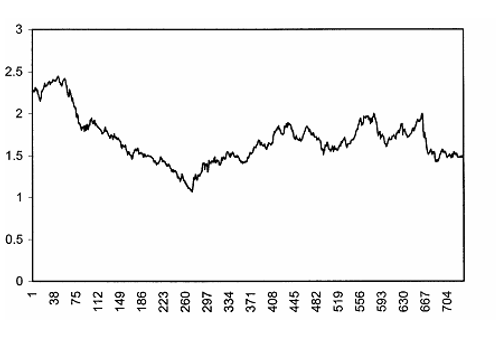
\includegraphics[width=0.8\linewidth]{project/fd.PNG}

\caption{Weekly BP/USD exchange rate series (1980-1993)}
\end{figure}
\begin{figure}[htbp]
\centering
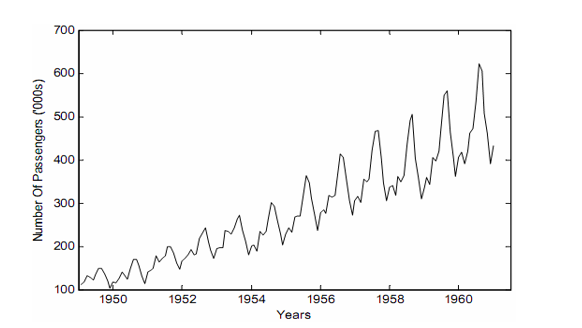
\includegraphics[width=0.8\linewidth]{project/fd1.PNG}

\caption{Monthly internation airline passenger series (Jan 1949-Dec 1960)}
\end{figure} The first Time-Series plot originates from the paper \cite{zhang2003time} and presents the weekly exchange rate between the US dollar (\$) and the GBP (\pounds) for the specified time between 1980 and 1933. The second plot presents seasonal Time-Series data and show on monthly basis, the number of worldwide airline passengers between January 1949 and December 1960 as examined in paper \cite{adhikari2013introductory}.
\textbf{Time-Series Analysis} is the procedure of fitting an appropriate Time-Series model on known data and estimating the relevant model's parameters. In Time-Series analysis, we gather past observations in order to construct an appropriate mathematical model that captures in the best way data patterns and their nature. Afterwards, the constructed model is used to predict the Time-Series' future values, which is a crucial procedure because business decisions and precautionary measures are obtained based on these forecasts .
\par Last but not least, we should have in mind that When constructing a Time-Series model we should incorporate the principle of \textbf{parsimony} \cite{provost2013data}. 
Under this principle, the model with the smallest number of parameters among the other candidate models should be preferred, nevertheless providing an accurate description of the associated Time-Series inherent features. In simple words, when you are requested to choose among a range of adequate explanations (models) of the Time-Series data, choose the simplest one. Furthermore, the more complex the model, the larger the risk of overfitting.
An over-fitted model performs very well on the training data, although it's not going to be accurate for forecasting. Having that in mind, parsimony principle is usually incorporated into the model, as a guide to prevent model overfitting. So to sum up, we should always choose the most parsimonious model between the available candidates when constructing forecasting models.

\chapter{Time Series Forecasting using ARIMA \& SARIMAX models}
Selecting the appropriate model for fitting the data is a procedure of high importance, because it mirrors the underlying structure of the time-series and  the produces the future forecasts. A time-series model may be labeled as linear or non-linear depending on whether each value of the time-series is a linear or non-linear function of the previous observations. Generally, time-series models may have numerous forms and illustrate different stochastic processes. Autoregressive moving average models fall into the category of stochastic models and their main objective is to describe the evolution of a phenomenon based on the time. Since it is not possible to record all the factors that affect load evolution over time, it is very difficult to be described by a deterministic model. Yet the choice of a stochastic model, such as ARIMA, is satisfactory as load demand depends on non-deterministic factors, such as weather or any random events, and a description of load demand over time can be succeeded with this stochastic model.These stochastic models contain randomness (random error or prediction error), the values of the metric under study over time and in some cases other stochastic factors, thus the resulting model is a linear combination of the above mentioned terms \cite{kihoro2004seasonal}.
\par 
The most common linear time-series models are the AutoRegressive (AR) and Moving Average (MA) models. Moreover in literature, combinations of these two models the AutoRegressive Moving Average (ARMA) and the AutoRegressive Integrated Moving Average (ARIMA) models have been proposed.Due to their simplicity, intuitiveness and implementation, linear models have attracted a lot of attention nowadays. Nonetheless most of the time-series in real-life scenarios present non-linear patterns, such as stock price forecasting where non-linear models are considered to be more accurate for predicting volatility changes in economic time-series. So numerous non-linear time-series models have been proposed in literature and in this chapter we will introduce remarkable linear and non-linear stochastic time-series models and their salient features.
\section{ARMA \& ARIMA Models}
\par An ARMA model (p, q) is a combination of AR (p) and MA (q) models and is suitable for time-series modeling. An AR model (p) calculates the future value of the response variable as a linear combination of previous observations for that value and a random error factor together with a fixed term. Mathematically the model AR (p) can be formulated as \cite{contreras2003arima}:

$$y_t= c+\sum\phi_{i}y_{t-i}+\epsilon_t$$

\noindent where $y_t$ and t are respectively the actual value and random error in time period t, with i = 1, 2,... while p is a model parameter and c is a constant. Integer constant p is
referred to as the model's order. Furthermore, for the shake of simplicity the fixed term is omitted. In order to assess the parameters of an AR procedure based on the time-series data, we use the Yule-Walker equations .
\par On the other hand, just like an AR model (p) relates previous values in the series, an MA model (q) uses previous errors as variables. The model MA (q) is given by [12, 21, 23] and can be expressed using the following equation.
$$y_t= \mu +\sum\theta_{j}\epsilon_{t-j}+\epsilon_t=\mu +\theta_1\epsilon_{t-1} + \theta_2\epsilon_{t-2}.... +\theta_q\epsilon_{t-q} + e_t$$
\par By default, ARMA models should and can be used only for stationary time-series. Nevertheless, in real life scenarios most of the time-series data, such as those related to economics and operations present non-static behavior. Time-series data that contain trend and seasonal patterns, are also considerd to be non-stationary \cite{choi2012arma}. Thus, the ARMA models are not capable to properly describe the non-stationary time-series data, which are frequently found in real life case studies. In order to bridge that gap, the ARIMA model is therefore proposed, which is a generalization of an ARMA model aiming to overcome the phenomenon of non-stationarity. More specifically, in ARIMA models, a non-stationary time-series is converted to stationary by applying finite differentiation on the data. The ARIMA model is the most common forecasting technique for one-dimensional time-series data. Although the model can handle sufficiently non-stationary time-series data, it isn't capable of supporting seasonal time-series data. ARIMA works only with data that are either non-seasonal or seasonal data where the seasonality has been removed, thus turning the series into stationary. An extension to ARIMA that supports the modeling of the seasonal element of time-series is called SARIMA.
\section{SARIMA model}
The ARIMA models that we discussed above are intended only for non-seasonal data modeling. On the other hand, a seasonal ARIMA model is an enhancement of ARIMA models, created by incorporating additional seasonal terms to the widely spread non-seasonal ARIMA models. The previously mentioned ARIMA variation is referred to as SARIMA (p, d, q) (P, D, Q, m), where (p, d, q) is the non-seasonal part of the model, (P, D, Q, m) is the seasonal part of the model and finally m is the number of time steps for a single seasonal period \cite{bouzerdoum2013hybrid}. In other words, SARIMA introduces three new parametric elements in order to define AutoRegression (AR), Integration (I) and Moving Average (MA) concerning the seasonal nature of time-series, along with an additional parameter for the seasonality period.
In the following list, we present the SARIMA model parameters that require tuning:
\begin{itemize}
    \item p: Trend AutoRegression order.
    \item d: Trend difference order.
    \item q: Trend Moving Average order.
    \item P: Seasonal AutoRegression order.
    \item D: Seasonal difference order.
    \item Q: Seasonal Moving Average order.
    \item m: The number of time periods in each seasonal period.
\end{itemize}
\section{SARIMAX Model}
Last but not least, when including in our model external input variables, like temperature, atmospheric pressure, for example when we are dealing with time-series data concerning rain frequency, then we will use another variation of the ARIMA model that is called ARIMAX model and generally can be expressed with the following formula:
\begin{figure}[htbp]
\centering
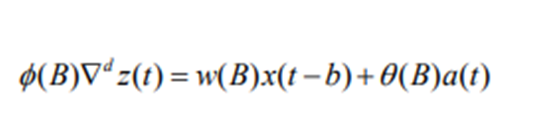
\includegraphics[width=0.6\linewidth]{project/ARIMAX.png}

\end{figure}
\newline where x(t) is the external variable in time t and
\begin{figure}[htbp]
\centering
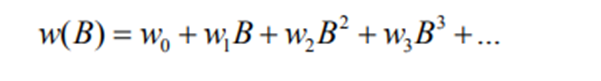
\includegraphics[width=0.6\linewidth]{project/w.png}

\end{figure}
When the ARIMA model contains seasonal variations and we have to include external variables in our model, then this variation is called SARIMAX. SARIMAX is essentially used in case the Time Series under study,  appears also seasonality except the trend. So in that case, the seasonal parameters are also included in the model and thus defining the Seasonal AutoRegressive Integrated Moving Average with eXogenous factor (SARIMAX (p, d, q)(P, D, Q, m)) \cite{tarsitano2017short}. \par Stohastic time-series modeling present numerous attractive features. The theory behind these models is well known, thus it's relatively easy to understand the forecasting procedure and its implementation. The model's parameters are relatively easy to tuned and moreover, the estimation of the white noise difference, creates a sense of confidence in the model's predictions. Furthermore, it is possible to establish diagnostic methods and the assessment of the model's parameters is clear. Forecasting time-series models containing exogenous variables, have been used for prediction in a vast variety of applications. Exogenous variables are also referred as covariates, which are considered as parallel input sequences referring to observations 
which follow the same time sequence as the actual time-series data. The actual time-series data may be referred to as endogenous sequence in contrary to the exogenous data sequence. Exogenous variables observations are incorporated directly in the model at each time step, although there are not configured in the same way as the primary endogenous sequence (e.g. as model AR, MA, etc.).
\par Last but not least, the application of ARIMA models presupposes the forecasting of short-term intervals. As mentioned earlier, these models are a linear combination of the historical time-series data. This means that if
we want to forecast the value Y on time t, then we have to know the values $Y_{t-1}$, $Y_{t-2}$. ARIMA models can be an excellent tool for understanding the evolution of values over time by analyzing and extrapolating them into the near future. ARIMA models deal with Time Series from a stohastic point of view and are based exclusively on the distribution of their past values and, above all, on the most recent ones \cite{arunraj2016application}. Our approach is based on a grid search approach, which tests
various model order configurations. The final model order is selected by
minimizing the Bayesian information criterion (BIC)
$$ BIC = AIC + (log(T) − 2)(p + q + k + 1)$$
Where AIC is the Akaike information criterion, which is defined as follows:
$$− 2log(L) + 2(p + q + k + 1)$$
where L is the value of maximum likelihood function of the model, k is the
number of model's parameters, p is the autoregressive order, q is
the model's moving average order and T is the number of observed samples. 
\chapter{Time Series Forecasting using the PROPHET algorithm}
\par 
Concerning the information used to provide the forecasts, there are two different approaches on time-series analysis. On the one hand, the standard approach includes only endogenous variables, while on the other hand the second approach incorporates exogenous variables also. The number of primary forecasting models is limited, whereas recent surveys have shown that the quality of forecasting could barely improved in the long term by switching between forecasting algorithms. In contrary, Hong and Fan (2016) underline that including appropriate exogenous forecasting variables could significantly improve the model's accuracy. The exogenous predictive variables that will be used to solve a particular forecasting problem could be derived from large-scale comparisons. Such comparisons facilitate benchmarking and model evaluation,i.e procedures requiring large amounts of data.
\par The Prophet algorithm -developed by Facebook- is a process for forecasting time-series data based on an additive model where non-linear trends match annual, weekly or daily seasonality and holiday too. \cite{taylor2018forecasting}. Prophet tends to work best with time-series data that present strong seasonal effects and considerable amount of historical data are available. The algorithm is thought to be very robust concerning lack of data, shifts the trend and usually it produces good results. According to the article on Facebook Research, Prophet was initially developed aiming to produce highly accurate forecasts to several business needs. This library tries to address the following difficulties common to many business Time Series: 
\begin{itemize}
    \item Seasonal effects caused by human behavior: weekly, monthly and yearly cycles, dips and peaks on public holidays
    \item Changes in trend due to new products and market events and 
    \item Outliers
\end{itemize}
Furthermore, the authors claim that, even with the default settings, in many cases, their library produces forecasts as accurate as those delivered by experienced analysts. Moreover, Prophet has a number of intuitive and easily interpretable customizations that allow gradually improving the quality of the forecasting model. What is especially important, these parameters are quite comprehensible even for non-experts in Time Series analysis, which is a field of data science requiring certain skill and experience. By the way, the original article is called "Forecasting at Scale", but it is not about the scale in the "usual" sense, that is addressing computational and infrastructure problems of a large number of working programs. According to the authors, Prophet should scale well in the following 3 areas:
\begin{itemize}
    \item Accessibility to a wide audience of analysts, possibly without profound expertise in Time Series.
    \item Applicability to a wide range of distinct forecasting problems.
    \item Automated performance estimation of a large number of forecasts including flagging of potential problems for their subsequent inspection by the analyst.
\end{itemize}
\par It has been observed that Prophet algorithm with it's default settings, tend to generate forecasts quite accurate with considerably less effort in contrary with more advanced forecasting algorithms. In case the Prophet algorithm provides bad forecasts you don't have to do with a black box procedure, because with even no training in time-series analysis we can improve the model's forecasting ability just by tuning it's parameters \cite{park2019144}. We observed that a wide variety of business scenarios can be addressed by combining automated forecasting processes in conjunction with an analyst-in-the-loop for extremely special forecasting tasks. The following diagram \cite{taylor2018forecasting} presents the forecasting method observed to operate efficiently at scale:
\begin{figure}[htbp]
\centering
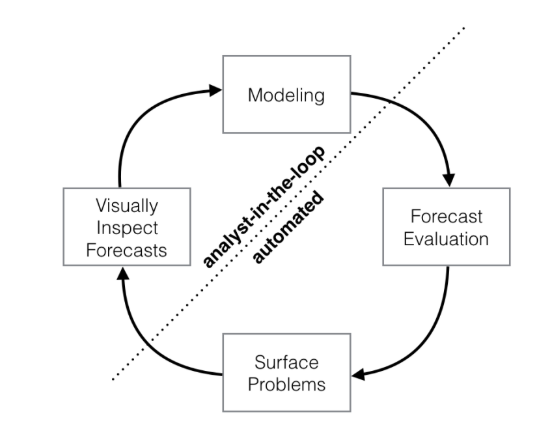
\includegraphics[width=0.8\linewidth]{project/prophet.PNG}

\caption{Automated forecasting process with analyst-in-the-loop}
\end{figure}
Prophet has been oftenly used as the main forecasting algorithm in numerous case studies based on the following two benefits:
\begin{itemize}
    \item It's much more genuine to generate reasonable and accurate forecasts with Prophet
    \item Prophet incorporates numerous different forecasting algorithms, such as ARIMA, exponential smoothing, etc, and also provides the ability for parameter tuning.
\end{itemize}
In general, selecting the wrong model or not the optimal parameter values, could sometimes generate poor forecasts, and even experienced data analysts may not be able to select the optimal model and its parameters, having in mind the variety of choices. As mentioned earlier, Prophet models may be easily customized by non-experts also, as smoothing parameters for seasonality and trend are provided, thus allowing the user to adjust the degree of how abruptly the algorithm follows trend changes and historical cycles. The principal concept in Prophet, is that by flexibly fitting the trend component and accurately modeling seasonality, we tend to generate more accurate forecasts. For tasks such as curve-fitting, we prefer to use flexible regression models instead of a traditional time-series models because it provides more modeling flexibility, thus making it straightforward to fit the model, handle missing data and outliers.
\par Accordingly, Prophet generates uncertainty intervals for the trend component by simulating future trend changes to the time-series data. In case of uncertainty modeling concerning future seasonality or holiday impacts, the user can run numerous Hamiltonian Monte Carlo (HMC) iterations and the results will incorporate seasonal uncertainty estimations. When we try to forecast a measures growth, such as total population, a maximum achievable point exists which is referred to as carrying capacity. Prophet is capable of generating forecasts by utilizing a logistic growth trend model bounded by a specified carrying capacity \cite{tyralis2018large}. The Prophet forecasting algorithm is provided in Python and R and predicts future timeline values by utilizing machine learning algorithms.The Prophet algorithm is considered as an additive regression model with the following four principal components: 
\begin{enumerate}
    \item A piecewise linear or logistic growth curve trend (Prophet identifies trend changes by specifying data change points)
    \item an annual seasonal term modeled using Fourier series
    \item a weekly seasonal term using dummy variables
    \item a user-provided array containing holidays 
\end{enumerate} 
The parameters used in the algorithm, are customized such as to match every possible time-series provided as input. It includes several parameters that can either be given by the user as fixed or can be given with specific limits that give the algorithm full freedom to select the parameter's optimal values. The mathematical relationship that describes the algorithm output is shown below \cite{taylor2018forecasting}:
$$y(t)=g(t)+s(t)+h(t)+\epsilon(t)$$
\noindent where the above functions denote:
\begin{itemize}
    \item g(t): Models trend component in time-series, by including two different models. A piecewise linear model and a saturating growth model, based on the forecasting scenario under study.
    \item s(t): Models seasonality by utilizing Fourier series, which describes how time-series is influenced by seasonal factors.
    \item h(t): Models the holiday effect and other extreme events that impact time-series data.
        \item $\epsilon(t)$: The error term.
\end{itemize}
\par Each of these four terms is responsible for modeling and simulating a different parameter that contributes to our result and predicting the next day value of the Time Series. For periodic changes s(t), they use Fourier transformation and the search of the optimal coefficients is being left to the algorithm. Moreover, functions like g(t) are being simulated with logistic regression models with small changes and also with the introduction of additional parameters that are either fixed or time-related functions. Concerning h(t) function, it is responsible for being able to identify which periods are holiday and to influence the equation accordingly. For the more correct use of this function, the algorithm -before running- gives the user the choice to enter his country's holiday. 
Concerning the term e(t), it is a function which affects our result according to the data under examination. In particular, it tries to perceive patterns or anything else that affects our outcome and cannot affect any of the previous three functions. These functions are characterized by a large number of parameters which can either be introduced by use or give the algorithm the freedom to calculate them to minimize the error of forecasts. The error term  $\epsilon(t)$  represents information that couldn't be explained by the model and thus it is included in the model as noise.
\par Time-series data in the real world, often present abrupt changes on their trajectories, then Prophet will automatically identify these changepoints allowing the trend component to adapt appropriately \cite{chen2009overview}. Prophet identifies these changepoints by first specifying numerous potential changepoints, where rate change is allowed. Following that, applies a sparse prior on the magnitudes of the rate changes (similar to L1 regularization). In other words, Prophet detects numerous possible data points where the rate could change, but will use just a subset of them as potential changepoints. Regarding seasonality and special days, Prophet detects seasonality based on partial Fourier sum, where the number of included terms is specified by a parameter that determines defines how rapidly the seasonality can change. In contrary, when holidays should be modeled, its compulsory to define a new dataframe, which must include holiday occurrences, both in the past and in the future, as the forecasting horizon dictates. Last but not least, it is worth to mention that Prophet algorithm was designed by Facebook company and the algorithms' parameters have been tuned based on the distributions that company's data follow, which may not be the case in every Time Series that we try to apply to this algorithm. 
\chapter{Time Series Forecasting using Neural Networks}
\section{Basic Concepts of Neural Networks}
By default, the main characteristic of neural networks is their ability to learn. In layman’s terms, when a neural network is learning it improves its ability to solve a problem through a repetitive process of gradually adjusting the neuron weights to the appropriate values that achieve the solution to the problem. Consecutively, by the end of the training step these parameters will get a fixed value. The challenging part is to achieve generalization \cite{liu2018r}. Generalization is the phenomenon where the neural network is general enough to be able to give appropriate outputs for inputs other than those it was trained for. Furthermore, neural networks provide another way of finding non-linear hypotheses since they decide to include ordered terms that best fit the data.
Neural networks emulate the way the brain works and its learning procedure. In correspondence to a human’s brain, the neuron is the basic building block and it consists of the axon, the dendrites and the synapses. The axon is the neuron exit gate and sends signals to other neurons, the dendrites are the neuron entry gates, and the synapses are the points of union between the neuron and the other neurons' dendrites. Neuron studying and the mathematical modeling of their structure led to artificial Neural Networks. The McCulloch-Pitts model as seen in the following figure \cite{chakrabortyoptimized}, is a simple model for describing the neuron.
\begin{figure}[ht!]
\centering
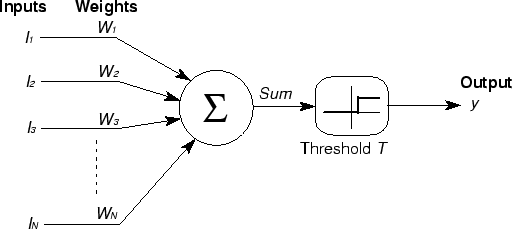
\includegraphics[width=0.6\linewidth]{project/Pitts.png}

\caption{The McCulloch-Pitts Neuron model}
\end{figure}
\par As seen above, $I_1, I_2, I_3 ...I_N$ are the neuron inputs and $w_1, w_2, w_3...w_N$ are called synaptic weights. If the sum of the products $I_i*W_i$ is greater than the T threshold, then the neuron passes the sum into the output y, otherwise it remains inactive. 
In an effort to accurately simulate the brain’s functionality, “Artificial Neurons” are a simplified version of the biological ones. The inputs are represented by $x_{i}$. Each input is multiplied by some weight $w_{i}$, and all $w{i}*x{i}$ products are added. Following this step, the processed input is fed into an “activation function” which creates the output value, called “activation” value. Finally, there is an output path. There is a number of Neural Networks architectures that are characterized by the differences in their activation functions. The most common one is the Sigmoid activation function $f(u)=1/(1+ \epsilon^{-u})$. More specifically, the activation function can be step transfer function, a linear transfer function, a non-linear transfer function or a stochastic transfer function. These artificial neurons can be connected in many ways to give “artificial neural networks”. The way that the network is structured is referred to as the network’s architecture. A network can be divided into different layers where the first and last one of them are called input and output layers, respectively. The layers in between are referred to as hidden layers and their number can arbitrarily large or small. It is important to point out though that layers only pass values forward and not backwards. Adding layers to the network increases its depth, as well as its accuracy. In such a network, there is one input layer, one or more hidden layers, and one output layer, as shown in the below figure \cite{liu2018r}. The layers in between are called hidden layers because they are hidden from the user.
\begin{figure}[ht!]
\centering
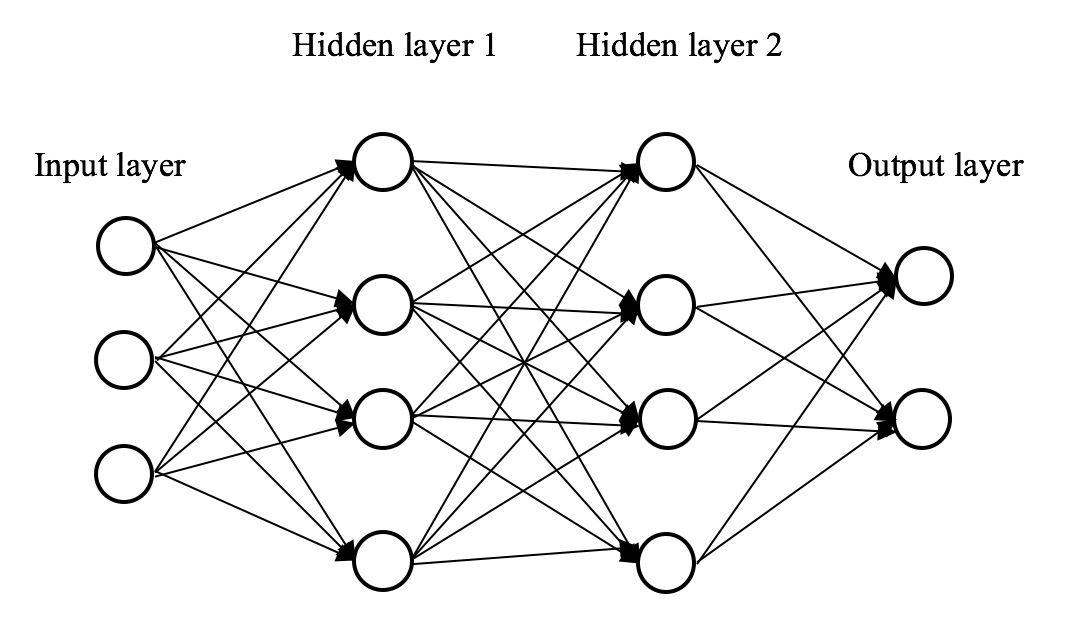
\includegraphics[width=0.8\linewidth]{project/testw.JPG}

\caption{Artificial Neural Network's Architecture}
\end{figure}
\par Usually in a neural network, each node in the previous layer is connected to every node in the following layer. Those created paths carry weights that the signal must be multiplied by when moving from one node to the other. This product is what reaches the end node. Each node receives several of these products from the nodes in the previous layer that connect to it. It sums them all up, applies the logistic function and passes the output forward to the next layer where the process repeats. Neural networks learning ability results from the tuning of the weights for each path so that the output layer produces a hypothesis that can model your data. In this way, complex non-linear hypotheses can be formed and the more hidden layers you have the potentially more complex models can be generated. 
\par Neural networks can (accurately) predict an output upon receiving some input. Broadly, a neural network consists of four components:
\begin{itemize}
    \item Artificial Neurons.
    \item Topology-how the neurons are connected
    \item Weights.
    \item Learning algorithm.
\end{itemize}
\par In the same way as every machine or deep learning algorithm, neural networks have to be trained on a dataset before they can be used to predict an output. Usually, the dataset consists of pairs of input-output. As a first step during training, all weights are randomly initialized and then the inputs are forward fed through the network to finally produce the output (“forward pass”) \cite{nicholson2019beginner}. Of course, the output of every node in each hidden layer takes into consideration the activation function for the calculations. The arbitrary weight initialization is bound to result in inaccurate outputs and thus the goal is to calculate the weight values that can successfully predict them with reasonable accuracy. The algorithm used to do this is known as “Backpropagation”. After the forward pass, we have some activations at the output layer.  An ideal neural network will result in outputs that are equal to the intended targets (known outputs). In practice this is not always the case and especially when the weights are randomly initialized. To account for that fact, the error is calculated using the “cost function” and then it is “backpropagated” through the network. As mentioned earlier, the goal is to adapt the weights so that the solution to the optimization problem of minimizing the cost function through “gradient descent” is acceptable. The plot of cost function vs weight is more or less convex and looks something like the following figure \cite{cost}.
\begin{figure}[ht!]
\centering
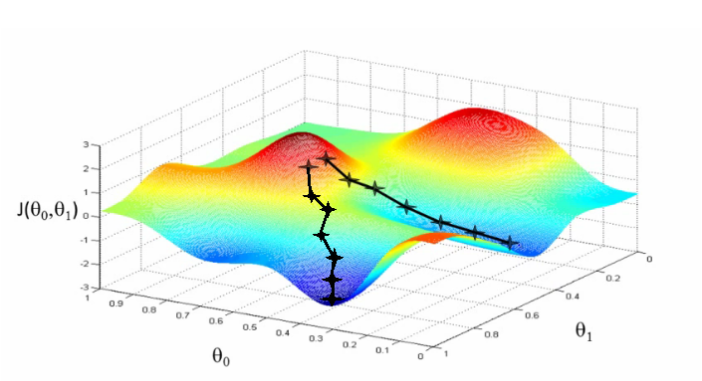
\includegraphics[width=0.6\linewidth]{project/convex.PNG}

\caption{Cost function and Gradient Descent}
\end{figure}
Gradient descent operates under the assumption that we make small steps towards the global minimum of the gradient when the plot is convex. In case the plot is not completely convex, we consider that the local minima are a good approximation of the global one. So we make small updates on the weights by multiplying them with the “learning rate” parameter, each time moving them in the direction of the gradient. Neural networks are highly sophisticated non-linear modeling techniques, capable of modeling extremely complex functions \cite{dilhani2017effect}. Keeping that in mind, they still fail to model complex phenomena where the popular linear models and their well-known optimization strategies are also straggling to show valid results. Of course, the problem on these types of networks is located on the dimensionality of the inputs and the outputs which could be an issue for large number of variables.
\par As a matter of fact, the manner in which the neurons of a neural network are structured is intimately linked with the learning algorithm used to train the network. For instance, in \textbf{Feedforward Neural Networks} the information flow is strictly moving from the input layer to the output. In addition, in the \textbf{Single Layer Feedforward Networks} example the term “single” refers to the output nodes where the inputs are fed directly via a number of weights.
More specifically, the feedforward network architecture utilizes a supervised learning approach to solve the issue of teaching it to perform well for a problem. Therefore, the inputs are fed into the network to produce the outputs through a pattern recognition process that indicates an input image of a “cat” or “elephant”, for example. As mentioned earlier, the goal is to train the network until it has the minimum category guessing error. With the trained set of parameters (or weights, collectively known as a model), the network sallies forth to categorize data it has never seen. An interesting advantage of this network architecture is the lack of time order perception. To be more precise, a trained feedforward network evaluates only the current input example and it will not assume that the next output is somehow dependent on the one under evaluation. A simple example is that seeing a photograph of a cat will not lead the network to perceive an elephant next \cite{grus2019data}.
\par A \textbf{Multilayer Feedforward Neural Network} is architected with a number of hidden units-neurons that formulate its hidden layers. The term “hidden” is used just because they do not have an immediate connection with the input or output layers and their main functionality is to help transform the input into the output in a more elaborate-meaningful kind of way \cite{gupta2018fundamentals}. By adding one or more hidden layers, the network is enabled to extract higher-order statistics from its input. Finally, another special Neural Network architecture is the \textbf{Recurrent Neural Networks (RNN's)}.
\begin{figure}[ht!]
\centering
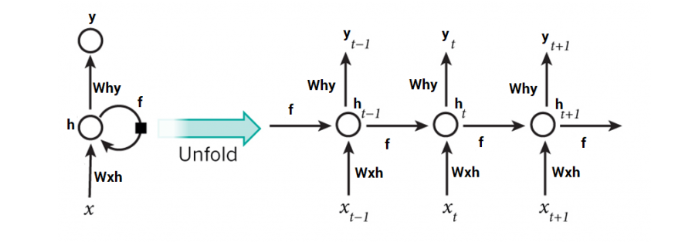
\includegraphics[width=0.8\linewidth]{project/rnn.png}
\caption{Unfolded basic Recurrent Neural Network}

\end{figure}
A recurrent neural network differs by having at least one feedback. Feedforward networks are amnesiacs regarding their recent past. There are no self-feedback loops in the network. The feedback loops involve the use of particular branches composed of unit-time delay elements, which result in a nonlinear dynamic behavior as shown in the figure below \cite{gupta2018fundamentals}.
\section{Long Short-Term Memory Units (LSTMs)}
Recurrent networks, in a sense, use a combination of inputs since they not only take into account the current ones but also the ones fed immediately before into the network. As a matter of fact, the decision a recurrent neural network reached at time step t-1 affects the decision it will reach one moment later at time step t. This is a distinguishable characteristic that separates recurrent from feedforward networks, a perception of “memory” as seen on figure 7.5 \cite{olah2015understanding}. \textbf{Adding memory to neural networks has a purpose: There is information in the sequence itself, and recurrent networks use it to perform tasks that feedforward networks can’t.}
\begin{figure}[ht!]
\centering
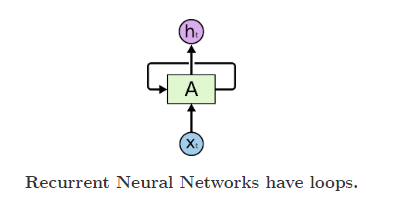
\includegraphics[width=0.7\linewidth]{project/rnn2.png}
\caption{Recurrent Neural Network loop}

\end{figure}
That sequential information is preserved in the recurrent network’s hidden state, which manages to span many time steps as it cascades forward to affect the processing of each new example. It recognizes correlations between events separated by many moments, and these correlations are called “long-term dependencies”, because an event downstream in time depends upon, and is a function of, one or more events that came before. 
\par RNNs can be considered as a mechanism to share weights over time. The information travel in the hidden states of the recurrent networks and the phenomenon can be described mathematically as follows. The hidden state at time step t is $h_{t}$. It is a function of the input at the same time step $x_{t}$, modified by a weight matrix W (like the one we used for feedforward neural networks) added to the hidden state of the previous time step $h_{t-1}$ multiplied by its own hidden-state-to-hidden-state matrix U, otherwise known as a transition matrix and similar to a Markov chain. The weight matrices are filters that determine how much importance to accord to both the present input and the past hidden state. The error they generate will return via backpropagation and be used to adjust their weights until error can’t go any lower. The sum of the weight input and hidden state is squashed by the function $\phi$ – either a logistic sigmoid function or tanh, depending – which is a standard tool for condensing very large or very small values into a logistic space, as well as making gradients workable for backpropagation \cite{palchak2013artificial}.
Because this feedback loop occurs at every time step in the series, each hidden state contains traces not only of the previous hidden state, but also of all those that preceded $h_{t-1}$ for as long as memory can persist. Given a series of letters, a recurrent network will use the first character to help determine its perception of the second character, such that an initial q might lead it to infer that the next letter will be u, while an initial t might lead it to infer that the next letter will be h.
\par The main perk of RNNs is the fact that they have the ability to combine previous information with a task at hand. This is a very useful characteristic that needs to be used carefully since not always do we have a problem that requires this combination of past and present knowledge. For example, consider a language model trying to predict the next word based on the previous ones. If we are trying to predict the last word in “the clouds are in the sky,” we don’t need any further context – it’s pretty obvious the next word is going to be sky. As a result, RNNs are able to learn and use the previous information needed to find the word. Their ability though is not limitless since as the learning time window increases RNNs are rendered unable to make connections with past information. Consider trying to predict the last word in the text “I grew up in France… I speak fluent French.” Recent information suggests that the next word is probably the name of a language, but if we want to narrow down which language, we need the context of France, from further back \cite{tripathi2008short}. 
\par The aforementioned phenomenon of short memory for RNNs is the result of the problem of Vanishing Gradient that also affects feedforward neural networks. This term is used to describe the fact that the gradient almost vanishes due to the small values of the activation functions derivatives that get multiplied multiple times as we move towards the starting layers. RNN remembers things for just small durations of time, i.e. if we need the information after a small time it may be reproducible, but once a lot of words are fed in, this information gets lost somewhere. 
In theory, RNNs are absolutely capable of handling such “long-term dependencies.” In practice, on the other hand, extensive research and literature suggests that this is not the case.
\par To solve this problem, a special family of RNNs was created and is called Long Short Term Memory networks or LSTMs. LSTMs are explicitly designed to avoid the long-term dependency problem. Remembering information for long periods of time is practically their default behavior, not something they struggle to learn. RNNs network architecture resembles a chain of repeating modules that are comprised of a simple structure. LSTMs build on that simple structure and instead of having just one neural network layer, they have four mingling in a particular way. The key to LSTMs is the cell state, the horizontal line running through the top of the diagram 7.6  \cite{olah2015understanding}. The cell state is kind of like a conveyor belt. LSTMs use this mechanism to move information around. We may have some addition, modification or removal of information as it flows through the different layers.
\begin{figure}[ht!]
\centering
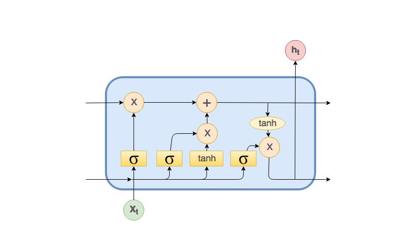
\includegraphics[width=0.7\linewidth]{project/lstm.png}

\caption{Inner structure of an LSTM unit}
\end{figure}
It runs straight down the entire chain, with only some minor linear interactions. LSTMs use gate structures to manipulate the information on the cell state. Even though information can run through unchanged, it can also be enriched or simplified this way. In general, gates are a way to optionally let information through. They are composed out of a sigmoid neural net layer and a pointwise multiplication operation. The sigmoid layer outputs numbers between zero and one, describing how much of each component should be let through. This way, LSTMs can selectively remember or forget things. The information at a particular cell state has three different dependencies.
These dependencies can be generalized to any problem as:
\begin{itemize}
    \item The previous cell state (i.e. the information that was present in the memory after the previous time step)
    \item The previous hidden state (i.e. this is the same as the output of the previous cell)
    \item The input at the current time step (i.e. the new information that is being fed in at that moment)
\end{itemize}
\par Now let’s get into the details of the architecture of LSTM network as seen in the following figure \cite{olah2015understanding}:
\begin{figure}[ht!]
\centering
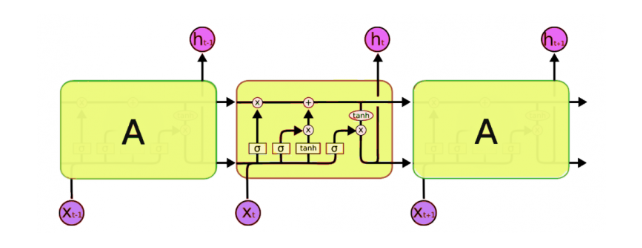
\includegraphics[width=1\linewidth]{project/archi.png}

\caption{LSTM Network Architecture}
\end{figure}
 A typical LSTM network is comprised of different memory blocks called cells (the rectangles that we see in the image).  There are two states that are being transferred to the next cell; the cell state and the hidden state. The memory blocks are responsible for remembering things and manipulations to this memory is done through three major mechanisms, called gates.

\bigskip
\textbf{Forget gate}
As the name indicates, a forget gate is used to remove information from the call state. This is a much-needed optimization technique for LSTMs since information that is no longer needed or of less importance is filtered out.
This gate takes in two inputs; $h_{t-1}$ and $x_t$.
$h_{t-1}$ is the hidden state from the previous cell or the output of the previous cell and $x_t$ is the input at that particular time step. The given inputs are multiplied by the weight matrices and a bias is added. Following this, the sigmoid function is applied to this value. The sigmoid function outputs a vector, with values ranging from 0 to 1, corresponding to each number in the cell state. Basically, the sigmoid function is responsible for deciding which values to keep and which to discard. This vector output from the sigmoid function is multiplied to the cell state \cite{lewis2016deep}.

\bigskip
\textbf{Input Gate}
The input gate is responsible for the addition of information to the cell state. This addition of information is basically three-step process as seen from the diagram above.
\begin{enumerate}
    \item Regulating what values need to be added to the cell state by involving a sigmoid function. This is basically very similar to the forget gate and acts as a filter for all the information from $h_{t-1}$ and $x_{t}$.
    \item Creating a vector containing all possible values that can be added (as perceived from $h_{t-1}$ and $x_{t}$) to the cell state. This is done using the tanh function, which outputs values from -1 to +1.  
    \item Multiplying the value of the regulatory filter (the sigmoid gate) to the created vector (the tanh function) and then adding this useful information to the cell state via addition operation.
\end{enumerate}
Once this three-step process is done with, we ensure that only that information is added to the cell state that is important and is not redundant.

\bigskip
\textbf{Output Gate}
The job of selecting useful information from the current cell state and showing it out as an output is done via the output gate. The functioning of an output gate can again be broken down to three steps:
\begin{enumerate}
    \item Creating a vector after applying tanh function to the cell state, thereby scaling the values to the range -1 to +1.
    \item Making a filter using the values of $h_{t-1}$ and $x_t$, such that it can regulate the values that need to be output from the vector created above. This filter again employs a sigmoid function.
    \item Multiplying the value of this regulatory filter to the vector created in step 1, and sending it out as a output and also to the hidden state of the next cell.
\end{enumerate}
\par LSTMs contain information outside the normal flow of the recurrent network in a gated cell. Information can be stored in, written to, or read from a cell, much like data in a computer’s memory \cite{franccois2017deep}. The cell makes decisions about what to store, and when to allow reads, writes and erasures, via gates that open and close. Unlike the digital storage on computers, however, these gates are analog, implemented with element-wise multiplication by sigmoids, which are all in the range of 0-1. Analog has the advantage over digital of being differentiable, and therefore suitable for backpropagation. Those gates act on the signals they receive, and similar to the neural network’s nodes, they block or pass on information based on its strength and import, which they filter with their own sets of weights. Those weights, like the weights that modulate input and hidden states, are adjusted via the recurrent networks learning process. That is, the cells learn when to allow data to enter, leave or be deleted through the iterative process of making guesses, backpropagating error, and adjusting weights via gradient descent. The figure below \cite{nicholson2019beginner} illustrates how data flows through a memory cell and is controlled by its gates.
\begin{figure}[ht!]
\centering
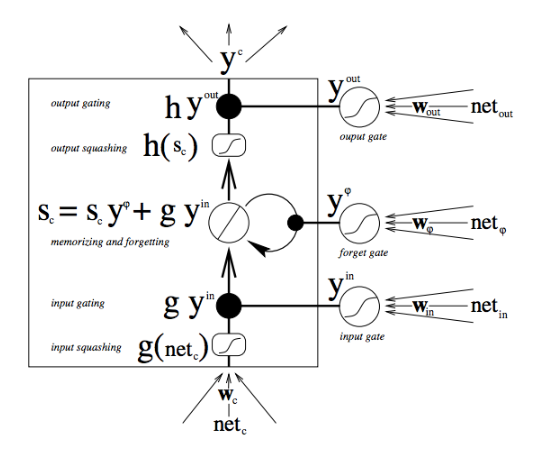
\includegraphics[width=0.6\linewidth]{project/a.png}

\caption{Data flow inside LSTM memory cell}
\end{figure}
\par Starting from the bottom, the triple arrows show where information flows into the cell at multiple points. That combination of present input and past cell state is fed not only to the cell itself, but also to each of its three gates, which will decide how the input will be handled. The black dots are the gates themselves, which determine respectively whether to let new input in, erase the present cell state, and/or let that state impact the network’s output at the present time step \cite{kyriakides2007short}. $S_{c}$ is the current state of the memory cell, and $gy^{in}$ is the current input to it. Remember that each gate can be open or shut, and they will recombine their open and shut states at each step. The cell can forget its state, or not; be written to, or not; and be read from, or not, at each time step, and those flows are represented here. The large bold letters give us the result of each operation. It’s important to note that LSTMs’ memory cells give different roles to addition and multiplication in the transformation of input. The central plus sign in both diagrams is essentially the secret of LSTMs. Simple as it may seem, this basic change helps them preserve a constant error when it must be backpropagated at depth. Instead of determining the subsequent cell state by multiplying its current state with new input, they add the two, and that quite literally makes the difference. (The forget gate still relies on multiplication, of course.) Different sets of weights filter the input for input, output and forgetting. The forget gate is represented as a linear identity function, because if the gate is open, the current state of the memory cell is simply multiplied by one, to propagate forward one more time step.
\chapter{Time Series Forecasting using Random Forest}
\section{Basic Components of Random Forests}
Random Forest is an ensemble machine learning method that utilize
different decision trees and numerous statistical techniques, such as \textbf{Boosting} and \textbf{Bagging}, in order to perform either classification or regression forecasting tasks. The ensemble approach is a technique which incorporates the forecasts of several machine learning algorithms to make accurate forecasts than any individual model, thus a model consisting of numerous forecasting models is termed as an ensemble model. Together with boosting, bagging is one of the most commonly used ensemble strategies, in order to overcome high bias and high variance \cite{cutler2012random}. Boosting bears upon a category of algorithms, that utilize weighted average technique in order to produce strong learners. In simple words, boosting and “teamwork” are synonyms. More specifically, each one of the numerous running models, determines sequentially where the next running model is going to focus on, in terms of feature selection. So each model is learning from the previous one, thus boosting the learning process as the name indicates.
On the other hand, \textbf{Bagging} is a technique based on random sampling with replacement of a dataset's subset. In general, bagging is used for variance reducing for algorithms that present high variance, such as decision trees \cite{srivastava2014introduction}. In the above mentioned technique, each model runs independently and in the end model's outputs are aggregated without indicating any preference to a specific model. Instead of simply averaging the forecasts of the trees, a Random Forest incorporates the following two core concepts:
\begin{enumerate}
    \item Random sampling of the training set's data, when creating the trees.
    \item Random feature subsetting concerning node splitting.
\end{enumerate}
More specifically, a RF creates numerous decision trees and combine their forecasts, in order to conclude in a prediction, that is more reliable and accurate in contrary with just using an individual decision tree's forecast.
Each tree incorporated in a random forest model, is trained based on random sampling with replacement procedure, or in other words bootstraping, so some samples of the training set may be used more than one time in a single tree.
The basic concept is that by training each tree on random samples, even though each tree could appear high variance regarding a particular subset of the training data, the random forest will have lower variance overall however not at the expense of increasing the model's bias. Another principal idea of random forests, is the fact that to each tree in the forest, only a subset of the features is available to make a decision, during the splitting nodes procedure as shown in figure 8.1 \cite{rfr}.
\begin{figure}[htbp]
\centering
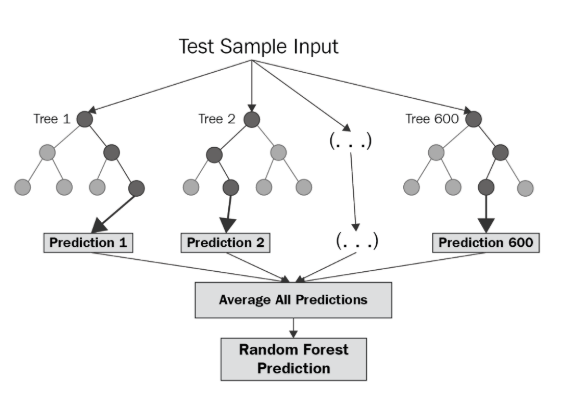
\includegraphics[width=0.7\linewidth]{project/rf.png}

\caption{Random Forest Structure}
\end{figure}
\par A good machine learning model's property, is the ability to generalize adequately to data that it has never seen before.
The phenomenon of overfitting is observed, when the training data are memorized by an elastic model, which leads to fitting it extremely closely.  Overfitting can create many complications in forecasting, because when overfitting exists, the model not only memorizes the dataset's actual relationships but also the model memorizes also the noise that may exist in the dataset. In flexible or elastic forecsating models, high variance is appearing because the parameters or in other words the decision tree's structure  will vary considerably with the training data. To the contrary, concerning inflexible models they present high bias, due to the fact that the models make assumptions about the training data. Moreover, in the end an inflexible model may not be able even to fit the available training data, thus whether the model presents high variance or whether the model presents high bias, the model is unable to generalize well to data never seen before.
\par 
The compromise among building a model that is so elastic that memorizes the training data as opposed to build an inflexible model that cannot be trained on the available data, is referred to as bias-variance tradeoff and is a fundamental concept in machine learning.
In the following sections, we will break down the Random Forest algorithm and explain bit-by-bit its process \cite{built}:
\begin{itemize}
    \item \textbf{Stage 1.} First of all, we sample repeatedly from the training set in order each observation in the dataset to have the same likelihood of being selected, having in mind that the sample size must be equal to the training set's size.
    \item \textbf{Stage 2.}  Then, based on the bootstrap samples collected in the previous phase, the Random Forest model makes the forecasts for each sample.
    \item \textbf{Stage 3.} Finally, the ensemble forecast is produced by averaging each one of the above tree's forecasts, thus resulting in the model final forecast.
\end{itemize}
\par The principal idea behind Random Forest algorithm, as we mentioned earlier, is the combination of the forecasts of numerous decision trees into one forecasting model. 
Individual forecasts provided by the numerous decision trees may be unreliable and incorrect, but when combined together after averaging the forecast, the final forecast will be closer to the actual observation. Each individual decision tree is trained on a different random sample of the training data, thus each tree contributes with a different way in the forecasting procedure. In case we used only an individual tree, we would incorporate in our forecast only the limited information contain available in that tree's training sample, whereas by combining numerous forecasts of the different available trees, the incorporated information on our final model would be greater thus making our forecasts more accurate. In case each individual tree used the same training sample, then the result would be very vulnerable to outliers, whereas the use of the forest and  different training samples results in more accurate overall predictions. Concerning forecasting, the Random Forest regressor averages individual trees forecasts, in order to reach the final forecast.
\par   In Random forests the individual decision trees run in parallel and furthermore no interaction exists between them. Random Forests run by building numerous decision trees during the training process and then produces the forecasts. In case the problem under study is a classification problem, then the Random Forest outputs the mode of the forecasted classes of all the individual trees, whereas when we are referring to a regression problem, the Random Forest outputs the predictions' mean based on the outputs of all the individual decision trees. Random Forests are also called meta-estimators, e.g they aggregate the result of multiple forecasts by combining multiple decision trees, with the following helpful modifications: \cite{srivastava2015tuning}
\begin{enumerate}
    \item The number of the available features that can be split on at each node, is constrained based on a certain percentage of the total amount of features. This certain percentage is part of a procedure that is called hyperparameter tuning. The above mentioned procedure guarantees that the ensemble model does not rely solely on any particular feature and that all possible predictive features are used sufficiently.
    \item During the splitting procedure, each individual tree selects from a random sample from the training set, thus adding a further apect of randomness in the model in order to prevent overfitting.
\end{enumerate}
\par One of the most accurate learning algorithms available in literature is Random Forests, concerning both Classsification and Regression tasks. Random Forests run efficiently on large databases and they are capable of handling thousands of input variables without removing features.
Furthermore, as the Random Forest building progresses, an unbiased calculation of the generalization error is generated.
Last but not least, they are capable of calculating missing data but also producing accurate forecasts even in case a large percentage of the data are missing. On the other hand Random Forests have some disadvantages too. Unfortunately, they tend to overfit when dealing with noisy datasets. Moreover, concerning data that include categorical variables with numerous levels, Random Forests have been observed to be biased towards features with more levels, thus making the variable importance scores unreliable \cite{casella2013springer}.
\section{Random Forest Regression}
As we have already mentioned, the Random Forest algorithm can also be applied to regression problems. In a classification task, the model allows predicting the existence of observations in a class, based on quantitative and/or qualitative variables. In regression (continuous response variable): The model allows the creation of a predictive model for a quantitative response variable based on quantitative and/or qualitative variables. Regression is a widely used statistical modeling technique which aims to examine the existence of correlation between a dependent variable and one or more independent variables. Regression assumes that certain data match some common types of functions and thereafter determines the function that models the given data optimally. Regression applications are the modeling of tasks such as load demand forecast, wind speed concerning temperature, humidity and other weather factors etc.
\par As we mentioned in the beginning, Regression is a widely used statistical modeling technique which aims to examine the existence of correlation between a dependent variable and one or more independent variables \cite{liaw2002classification}. Regression models include the following variable types:
\begin{itemize}
    \item Unknown correlation parameters declared as b (vector).
    \item Independent X variables (vector).
    \item The dependent variable Y or else the response variable.
\end{itemize}
A regression model associates Y dependent variable with X and b based on the regression function, H= F(X,b). Regression Analysis helps us understand the change in response variable Y when one of the independent variable X changes, while the other independent variables are kept constant. Usually, the causal effect of one variable on another is to be determined. Such an example, is the investigation of the impact of product price increase on supply/demand. In other words, we collect data concerning the variable of interest and then we run regression analysis in order to measure the quantitative effect of independent variables on the response variable. The statistical significance of the estimated correlation coefficients, e.g the confidence that the actual correlation value is close to the correlation that we estimated, is also assessed \cite{rfr}.
\par  Random Forests algorithm, uses a combination of the bagging algorithm and the random selection of variables in order to de-correlate individual decision trees. 
In the section below, we present the pseudo-code of Random Forests in order to understand bit by bit the different stages of the algorithm. \newpage
\lstset{ %
language=C,                % choose the language of the code
basicstyle=\footnotesize,       % the size of the fonts that are used for the code
numbers=left,                   % where to put the line-numbers
numberstyle=\footnotesize,      % the size of the fonts that are used for the line-numbers
stepnumber=1,                   % the step between two line-numbers. If it is 1 each line will be numbered
numbersep=5pt,                  % how far the line-numbers are from the code
backgroundcolor=\color{white},  % choose the background color. You must add \usepackage{color}
showspaces=false,               % show spaces adding particular underscores
showstringspaces=false,         % underline spaces within strings
showtabs=false,                 % show tabs within strings adding particular underscores
frame=single,           % adds a frame around the code
tabsize=2,          % sets default tabsize to 2 spaces
captionpos=b,           % sets the caption-position to bottom
breaklines=true,        % sets automatic line breaking
breakatwhitespace=false,    % sets if automatic breaks should only happen at whitespace
escapeinside={\%*}{*)}          % if you want to add a comment within your code
}
\begin{lstlisting}
Select the number of models to build, m
for i=1 to m do
   Generate a bootstrap sample of the original data
   Train a tree model on this sample
   for each split do
       Randomly select k(<P) of the original predictors
       Select the best predictor among the k predictors 
        and partition the data
   end
   Use typical tree model stopping criteria to determine 
   when a tree is complete (but don't prune)
end
\end{lstlisting}

Firstly, the algorithm determines the number of \textit{m} samples to be aggregated and thereafter all these \textit{m} forecasting models are aggregated thus providing a reliable forecasts with lower variance. Instead of selecting all the available features during the node splitting procedure, a random selection of k features among the total number of features at each split is performed. With this procedure we ensure that only the feature with the best splitting performance feature can be chosen to split the data, thus de-correlating the individual trees by introducing this kind of
randomness when building the individual trees. Concerning model tuning, there are two primary parameters in the Random Forest algorithm and more specifically these are: 1) the number of aggregated samples \textit{m} and 2) the number of randomly selected features, \textit{k}. In general, the bigger the number of trees, the heavier the computational burden. Intuitively, a Random forest with a large number of trees ( m $\geq$ 1000 ) is suggested with $k=\sqrt{p}$ or $k=log(p)$, where p is the total number of the dataset's features. This randomly selected features is a subset of the total number of available features and despite the fact that the number of trees m in Random Forest algorithm is much bigger than that in the bagging tree, the Random Forest is still considered a more efficient algorithm. Moreover, the Random Forests are also considered to be efficient, accurate and highly reliable and are capable of dealing with datasets containing numerous variables. Furthermore, the relative importance of predictors can be deduced, even if the correlation among predictions and the tuning parameter k affects heavily the forecast. Last but not least, the Random Forest algorithm can efficiently handle datasets with large number of missing data and provide higly accurate forecasts. On the other hand, Random Forests are not able to provide accurate forecasts when the response variable value to be predicted is out of the range of the observed values in the training data. 
\par The Random Forest Regression (RFR) algorithm was proposed and applied to quantify complex
nonlinear relationships without leading to the obvious overfitting risk \cite{segal2004machine}. RFR has been demonstrated
to be more computationally cost-effective than many popular machine-learning algorithms.
It has been widely used for predictions of stock price, electricity load demand, property sale price etc. The Random Forest Regression is a non-parametric ensemble learning algorithm that
constructs numerous standard decision trees during the training process and outputs mean prediction of
the individual trees, as seen in the following figure \cite{xu2019water}. 
\begin{figure}[htbp]
\centering
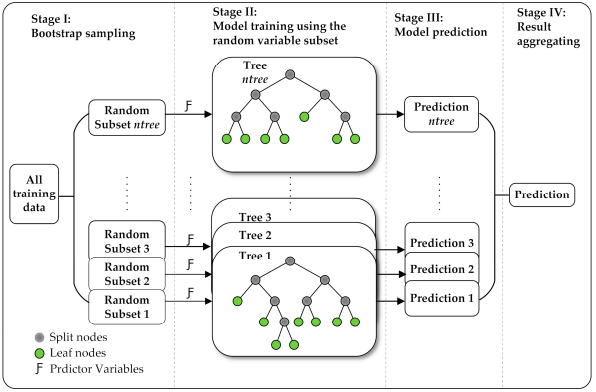
\includegraphics[width=0.9\linewidth]{project/rf2.PNG}

\caption{Random Forest Regression Algorithm}
\end{figure}
\newpage
A decision tree is a hierarchical analysis diagram where each internal (split) node represents a test function on one independent variable, each branch represents the test outcome and each terminal (leaf) node represents a decision. Specifically, at each internal node, the algorithm searches the values of the incoming dataset and recognizes a threshold for one predictor variable to split the dataset such that the homogeneity of dependent variable values in each branch is maximized. In the RFR, each decision tree is trained using a subset of data randomly sampled with replacement from the original training dataset, which can increase the robustness against overfitting. In order to inject an additional layer of randomness, instead of using all variables, only a subset of randomly selected variables are considered to form the split nodes of each tree. The reason to add this randomness is to reduce the redundancy of predictor variables while increasing the diversity of the individual trees in a forest \cite{breiman2001random}. The final result of RFR is decided by aggregating predictions of each individual tree. The RFR algorithm has four steps described as follows:
%\begin{enumerate}
%    \item Use the bootstrap method to produce $n_{tree}$ subset samples from the original training dataset,
%where $n_{tree}$ is the number of trees to grow.
%    \item Grow regression trees on each bootstrap sample, during which, randomly draw a subset
%containing $m_{try}$ predictor variables at each splitting node and determine the optimal split based
%on this subset of variables only. This process is conducted recursively until a stopping criterion
%(nodesize) is reached.
%    \item Obtain regression predictions over $n_{tree}$ decision trees. For each individual tree, the prediction is the mean of the response variable's values at the corresponding leaf nodes.
%    \item Compute the final prediction by averaging ntree predictions in the forest.
%\end{enumerate}
In the field of machine learning, a hyperparameter is a parameter whose value is tuned either to
improve model performance or to decrease the time and memory cost of running. The model
performance is the only aspect considered in this paper. The three main hyperparameters in RFR that
can influence the model’s performance are $n_{tree}$, $m_{try}$ and nodesize. As mentioned earlier, $n_{tree}$ is the
number of trees in a forest. Larger $n_{tree}$ can increase the stability of models and predictor importance estimates while decreasing the degree of overfitting, but requires more computational resources.
The second hyperparameter $m_{try}$ is the number of variables available for splitting at each tree node,
which determines the diversity among decision trees. Lastly, nodesize is the minimal size of the leaf
nodes, which is used as a stopping criterion and controls the depth of the trees. 
\par Two strategies are widely used to validate models when tuning hyperparameters in machine
learning \cite{sathyadevan2015comparative}. First is k-fold cross validation (CV), in which multiple rounds of validation are performed
using different partitions of a dataset, and the final result is averaged over the k rounds to evaluate
the model performance. The second strategy is to evaluate trained RFR using out-of-bag (OOB) data,
which is the data (approximately one third of total data) not drawn by bootstrapping for growing an
individual tree at the training stage. Usually, CV is more reliable since it overcomes the fact that the
model performance can be very sensitive to how training and validation subsets are divided, but OOB
requires shorter runtime. To reduce the risk of overfitting, this study combines these two strategies for
searching the optimal hyperparameter sets, which has two steps described as follows:
\begin{itemize}
    \item For each round of CV, tune hyperparameters using the grid search method to minimize the OOB
error within the training dataset.
    \item Assign the hyperparameter combinations with the lowest OOB errors to each of the k models
and test their performances using their corresponding validation datasets. The hyperparameter
combination that has the best model performance is the final model configuration.
\end{itemize}

\chapter{Gradient Boosting Machines: LightGBM}
\section{Basic Concepts of Gradient Boosting}
In literature, Boosting is thought to be a procedure for converting weak learners into strong ones. In
others words, Boosting is an ensemble method for increasing model's accuracy independently of associated learning algorithm. The principal idea behind Boosting, is that each tree is fitted on some different part of the training dataset, thus weak learners are trained in a sequential way, while in parallel each learner attempts to correct its predecessor forecast \cite{ligentle}. At every iteration, a new weak learner is trained with respect to the residual error of the whole ensemble till that moment. On the other hand, methods mentioned in the previous chapters, like Random Forests and Bagging are based on the concept of constructing an ensemble of models, where every individual model generates the forecast and then the ensemble of models just estimates the average of the forecasted values. Boosting technique authorizes ML models to increase their forecasting accuracy, nonetheless boosting algorithms are easy to implement and allows different model designs which makes the selection of loss function a matter of trial and error. In general, the selection of the loss function may be arbitrary and it's the researcher's responsibility, but we should have in mind that when the loss function is very simple - e.g squared-error- , the learning procedure could result in continuous error-fitting. 
\par The family of boosting techniques is based on numerous constructive strategies of ensemble formation and the underlying engine incorporated for Boosting algorithms can be one of the following:
\begin{itemize}
    \item AdaBoost (Adaptive Boosting)
    \item Gradient Tree Boosting
    \item XGBoost
\end{itemize}
In \textbf{Gradient Boosting Machines (GBM)}, the training procedure continuously fits models in order to generate more accurate forecasts. The principal concept of this algorithm is to constract new base-learners which are greatly correlated with the negative gradient of the ensemble's loss function. GBMs are highly flexible and customizable and furthermore they show substantial accuracy not only in real world scenarios but also in numerous machine-learning competitions. Although Random Forests conctruct an ensemble of deep independent trees, GBMs construct an ensemble of weak sequential decision trees, where each individual tree learns and improves on the previous tree. In the end, all these sequential weak learners (trees) form a powerful “committee” that in general provides very accurate forecasts \cite{mei2018short}.
\par The Gradient Boosting algorithm can be easily interpreted by firstly introducing the AdaBoost Algorithm. Gradient Boosting and AdaBoost, both add sequentially predictors to an ensemble where each one is correcting its predecessors. The main difference between Gradient Boosting and AdaBoost, is the way that the algorithms identify the shortcomings of the decision trees. AdaBoost model identifies the shortcomings by using large weight data points, whereas Gradient Boosting performs the same procedure by incorporating gradients in the loss function $y=ax+b+\epsilon$ where $\epsilon$ is the error term. A major diffrence is that Gradient Boosting fits the newly added predictor to the residual errors generated by the preceding predictors, where on the other hand AdaBoost adjusts the weights for each incorrectly forecasted observation at each iteration. Gradient Boosting repetitively leverages the patterns in residuals and when reaching a point that residuals do not follow any pattern that could be modeled, the modeling stops (in order to avoid overfitting). Last nut not least, one of the unique features of Gradient Boosting is the fact that allows the incorporation of a user-specified loss function, which may be more appropriate in real case scenarios.
In the following section, we will break down the GBM algorithm and explain step-by-step its process:
\begin{itemize}
    \item Fit a model, F1(x) = y
    \item Fit a model to the residuals, h1(x) = y−F1(x)
    \item Construct a new model, F2(x) = F1(x) + h1(x)
    \item Combine more and more weak learners sequentially, thus producing the final model able to account for a large amount of the original model's error and reduce this error as time passes by.
\end{itemize}{}

\section{Gradient Boosting Decision Trees}
Gradient Boosting Decision Trees (GBTS) combine the forecasts of numerous decision trees by adding them together, in order to provide forecasts that generalize well. GBTS is a computationally efficient technique to capture correlations/interactions among model's variables by utilizing decision trees. More specifically GBDTs are trained iteratively in a way that the GBDT forecasts the response variable by firstly training weak decision tree on the data. The above mentioned trees are parameterized by the number of splits, or in other words the interaction depth. Every individual split denotes the splitting rule over each explanatory variable, thus modeling the interactions among the input variables. Furthermore, each decision tree aims to minimize the specified error function by recursively splitting the data in such a way to maximize some criterion's threshold, like the tree's depth. That criterion is selected based on the idea, that the loss function is minimized in each split. Last but not least, estimating the best available split requires the decision tree to test various splits and calculate the criterion's value for each split \cite{cook2016practical}. 
\par A special case of decision tree with only one split or two terminal nodes is the so called tree stump, which  many practical applications small trees and tree-stumps provide considerably accurate results. 
Additionally, there is experimental evidence in literature that complex trees (e.g tree depth > 20) provide hardly any benefit in contrary with compact trees (e.g tree depth ≈ 5). It's worth noticing that we can fit an additive model of weak tree base-learners by utilizing tree stumps. A salient feature of DTs is that by default a single decision tree always extrapolates the loss function with the constant value. 
There are two approaches that can be incorporated when training each individual decision tree and splitting the data: \textbf{level-wise} and \textbf{leaf-wise}. The level-wise approach generates a balanced tree, where on the other hand the leaf-wise approach make the splitting that mostly reduces the error function.  Furthermore, the level-wise training approach resembles a form of regularized training since leaf-wise training method is able to construct any tree that level-wise training can ,thus making the model more flexible but also the risk of overfitting increases, whereas the opposite is not possible. To conclude, the main challenge in training a Gradient Boosting Decision Tree is the procedure of identifying the best split for each leaf, although no known method is able to identify the best split without having to go through all the feature's available observations \cite{boehmke2019hands}.
\newpage
\section{LightGBM}
The Gradient Boosting Decision Tree (GBDT) and more specifically one implementation of the GBMT algorithm - called XGBoost – is thought to be one of the best performing algorithms in Kaggle's machine learning competitions. Although XGBoost seemed to be the king of algorithms in Kaggle for the time being, a new challenger is rapidly gaining momentum and this is the \textbf{lightGBM}. This algorithm was released by Microsoft and is claimed to provide better forecasting performance for the same running time than XGBoost. LightGBM is an outstanding implementation that is very similar to XGBoost, but the main difference is in particular the way trees are formed. Light GBM is a fast, distributed, high-performance gradient boosting framework based on decision tree algorithm, that can be used for regression, classification and numerous other machine learning tasks. Since LightGBM is based on decision trees, it splits the tree by utilizing the leaf-wise approach having the best fit, whereas other boosting algorithms split the tree level wise. The leaf-wise approach can reduce the loss to a greater extent than the level-wise approach, thus provides very accurate forecasts. Furthermore, LightGBM, as it's name Light suggests, is \textbf{surprisingly fast}.
The utilization of Leaf-wise splits, increases model complexity and raise the risk of overfitting. As mentioned earlier, overfitting can be avoided by setting a threshold to the max-depth parameter (e.g the depth where splitting takes place) \cite{lfl}.

\begin{figure}[htbp]
\centering
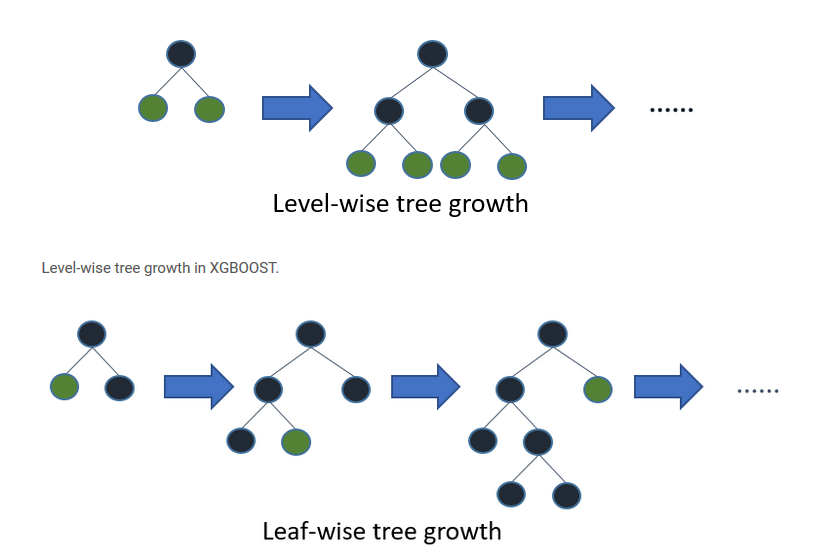
\includegraphics[width=0.75\linewidth]{project/LightGBM.PNG}
\caption{ Splitting data: Leaf-wise VS Level-wise}

\end{figure}


\par Numerous advanced users on Kaggle already incorporate LightGBM for each new competition, as it gets more and more coverage. Concerning parameter tuning, LightGBM offers some different parameters. but in general the majority of them are similar to their XGBoost counterparts. Concluding, we are going to list some of the LightGBM biggest advantages and these are \cite{NIPS2017_6907}:
\begin{itemize}
    \item Faster training and increased efficiency: LightGBM buckets continuous variables into discrete bins which makes the training procedure faster. In other words, LightGBM utilizes a histogram based algorithm.
    \item Reduced memory usage: Replacing continuous valuers to discrete bins, results in memory usage reducing.
    \item Higher accuracy: Due to the use of leaf-wise approach, it generates much more complex trees and this makes it more accurate than any other boosting algorithm by providing very accurate forecasts.
    Although, it should be noted that this approach can sometimes lead to overfitting which can be avoided by specifying the max depth parameter.
    \item Compatibility with large datasets: It's very efficient with large datasets, with a significant reduction in training time comparing to XGBoost.
    \item Parallel learning.
\end{itemize}

 \newpage   
\chapter{Forecast Performance Measures}
\section{Basic Concepts of Prediction Accuracy}
In simple words, when we are referring to "forecast accuracy", it's a measure to estimate how similar are the forecasted values in contrary with the actual ones. Concerning electric load demand time-series, this measure of "closeness" is calculated by forecasting load demand at referenced time. 
During the forecasting procedure, the actual values are unknown, but in order to select the optimal available algorithm and build our forecasting model, the model's accuracy is estimated by forecasting load demand for a past time interval, because actual historical data are available for the past. The above described procedure is called in-sample performance or exante analysis, in contrary with the out-of-sample performance or a posteriori analysis where the model's accuracy can only be evaluated after the forecasted fact takes place \cite{geron2019hands}.
In general, the are numerous factors that affect forecast's accuracy and most of them are listed below: 
\begin{itemize}
    \item \textbf{Volatility} of the forecasted phenomenon:
    Higher volatility index means reduced forecast accuracy.
    \item \textbf{Model Uncertainty-Overfitting}: When the same data used for fitting and testing, then bias exist in the model and the phenomenon of overfitting arise.
    \item \textbf{Aggregation}: According to literature, aggregating data leads to lower volatility in data, thus aggregating electric load demand over longer intervals (e.g. hourly instead of 15-minute intervals) leads to higher forecast accuracy. The above mentioned  aggregation procedure is referred to as temporal aggregation.
    \item \textbf{Forecast horizon length}: The further away we move from the forecast origin (the current time step), the more the forecast's accuracy decreases.
    \item \textbf{Algorithm selection}: A forecast model based on an algorithm that describes better the scenario under study, yields in more accurate forecasts.
\end{itemize}
The uncertainty around a forecasted value is expressed through the prediction interval. In simple words, the prediction interval defines in a probabilistic way the boundaries where the future observed values are expected to fall within. For example, for a 98\% prediction interval it is expected the actual observations to fall within, with a 98\% probability. A model's forecast evaluation, can be realized based on different accuracy metrics that consider forecast errors over the specified forecast horizon, summarized into a single value, which is called forecast performance measure or forecast accuracy metric. Counter intuitively we can understand that a lower accuracy measure means better prediction performance for the model \cite{armstrong1995correspondence}.
\newpage
\section{Forecast Performance Measures}
In the previous chapters, we studied various state of the art algorithms for time-series forecasting. Now the next step, is to apply these methods for building forecast models and making predictions. After creating a forecasting model but before applying the model to time-series data, we have to partition the data into two independent parts, the Training Set and the Test Set. The observations contained in the training set are used for constructing or in statistical language for fitting the selected model. In some cases, a small subpart of the data contained in the the Training set is kept for model validation purposes and this subpart is referred to as the Validation Set. Most of the times, after data transformations and preprocessing -such as log transformation, data scaling etc - is done the constructed model is used for making forecasts. The data contained in the Test set will be used for evaluating the accuracy of the fitted model when forecasting the observations in the test set. In order to evaluate the model's forecasting performance when comparing different models based on different algorithms, their relative forecasting performance on the test set is considered. We meet time-series tasks in many business situations, thus the importance of time-series forecasting and the optimal modeling of time series data is fundamental.
 Having that in mind, various forecasting accuracy measures, also referred as \textbf{performance metrics}, are proposed in literature in order to be able to compare forecasting models based on different algorithms. More specifically, these metrics are based on some function of the time-series' observed and forecasted values. In the following sections, we provide a brief description on the most common performance metrics used in literature and their notable features.  In each of the following formulas, $y_{t}$ is the observation's actual value at time t, $f_{t}$ is the forecasted value at time t, $e_{t}=y_{t}-f_{t}$ is the forecasting error and n is the size of the test set \cite{armstrong1992error}.
\subsection{MFE-Mean Forecast Error}
 The Mean Forecast Error(MFE) is the simplest scale-dependent accuracy metric and is formulated as $$MFE=\frac{1}{n}\sum_{t=1}^{n}{e_{t}}$$
 MFE detects bias in the forecasts (e.g overfitting), but when bias is not present in the forecast, it tends to ignore huge individual errors completely, due to the averaging process that takes place.
Some of the MFE's key features are: 
 \begin{itemize}
     \item MFE measures the average deviation between the actual values and the predicted ones. 
     \item MFE does not penalize large errors and moreover it is heavily depended on data scale and any data transformations. 
     \item MFE cancels out the sign of errors and we can not estimate their exact amount. In other words, a zero MFE does not mean that predictions contain no error but that errors cancel out.
     \item Last but not least, a good forecast means a MFE close to zero.
 \end{itemize}
\subsection{MAE-Mean Absolute Error}
Metrics that use absolute values of the forecasting errors, have the ability to detect the magnitude of errors in a more efficient way. Such a metric is the mean absolute error which is defined as follows:
 $$MAE=\frac{1}{n}\sum_{t=1}^{n}{|e_{t}|}$$  
Some of the MAE's key features are: 
 \begin{itemize}
    \item MAE measures the average absolute deviation between the actual values and the predicted ones. Thus MAE sometimes may be referred as Mean Absolute Deviation (MAD).
    \item MAE presents the magnitude of overall forecasting error, so positive and negative errors do not cancel out. 
    \item With MAE, due to absolute values, we cannot infer anything about forecasting error direction (over-predicting or under-predicting)
    \item A good forecast means a MAE as small as possible. 
    \item Last but not least, like MFE, MAE does not penalize large errors and it's heavily affected by data scale and data transformations. 
 \end{itemize}
\subsection{MAPE-Mean Absolute Percentage Error}
The mean absolute percentage error metric at time $t_{i}$ is scale-independent, so it's a suitable metric for evaluating a model's forecasting performance independently of the data under study. Furthermore, the MAPE, by using the absolute that we mentioned earlier, does not suffer from the deficit of Mean Percentage Error, where unless biases arise during the forecast, signed percentage errors will cancel out, resulting in inability to detect large percentage errors.
This measure is one of the most useful measures for practical purposes and its given by $$MAPE=\frac{1}{n}\sum_{t=1}^{n}{|\frac{e_{t}}{y_{t}}|*100}$$  
Some of the MAPE's key features are: 
\begin{itemize}
    \item MAPE denotes the percentage of average absolute forecasting error.
    \item MAPE is scale-independent, although it is heavily affected by data transformations. 
    \item With MAPE again due to absolute values, we cannot infer anything about forecasting error direction.  
    \item MAPE does not penalize extreme errors.
\end{itemize}
\subsection{MSE-Mean Squared Error}
The mean squared error (MSE) metric, measures the average squared difference between the forecasted values and the actual ones, or in other words MSE estimates the average of the squares of the forecasting errors.
The Mathematical formulation for this metric is expressed as $$MSE=\frac{1}{n}\sum_{t=1}^{n}{e_{t}^2}$$  Some of the MSE's key features are: \begin{itemize}
    \item MSE measures the average squared deviation between the actual values and the predicted ones.
    \item MSE gives an abstract idea concerning the forecasting errors, because the opposite signed errors do not cancel out.
    \item MSE due to forecast error squaring, is heavily affected by large errors and penalizes such occurrences during the forecasting procedure.
    \item With MSE we cannot infer anything about forecasting error direction and moreover MSE is sensitive to data scaling and transformations. 
    \item Last but not least, MSE may be a decent measure to estimate overall forecasting error, but it is not easily interpretable.
\end{itemize} 
\subsection{SSE-Sum of Squared Error}
SSE is the sum of the squared errors between the value of each observation and the observation's group mean value. SSE us mainly used as a measure of variation between observations belonging in the same cluster. In case all observations within a cluster are identical, then the SSE would then be equal to zero. The Mathematical formulation for this metric is expressed as $$SSE=\sum_{t=1}^{n}{e_{t}^2}$$  
SSE's key features are: 
\begin{itemize}
    \item SSE measures the total squared deviation between the actual values and the predicted ones.
    \item Concerning other properties, SSE presents the same properties as MSE. 
\end{itemize} 
\subsection{SMSE-The Signed Mean Squared Error}
The Signed Mean Squared Error metric is mathematically formulated as follows $$SMSE=\frac{1}{n}\sum_{t=1}^{n}{(\frac{e_{t}}{|e_{t}|})*e_{t}^{2}}$$
 and it's properties are: 
\begin{itemize}
    \item SMSE measures the same thing as MSE, but this time the error's sign  is preserved for each individual squared error. 
    \item SMSE penalizes large forecasting errors, but in contrary to MSE, from SMSE error metric we can infer the forecasting error's direction (over-predicting or under-predicting) 
    \item Last but not least, just as with MSE, SMSE measure is sensitive to data scaling and transformations.
\end{itemize} 
\subsection{RMSE-Root Mean Squared Error}
The root mean squared error (RMSE) is a quadratic scoring function that measures the forecasting error's average range, by calculating the square root of the average of squared deviations between predictions and then actual observations. The RMSE is expressed with the following formula $$RMSE=\sqrt{\frac{1}{n}\sum_{t=1}^{n}{e_{t}^2}}$$
The root mean squared error is just the square root of the calculated MSE, thus all the properties of MSE hold for RMSE as well. 
\par The right choice of the forecasting accuracy metric which will be later used to evaluate the forecasting models is highly significant. First of all, based on that metric we will choose the optimal forecasting model algorithm for our case study and furthermore it is important to mention that for different problems there may be different forecast accuracy metrics more suitable. The Mean Absolute Error (MAE) and the Root Mean Squared Error (RMSE) are the most commonly used and the most reliable measures concerning forecast evaluation of continuous variables, such as the electric load. Both MAE and RMSE express the model's average forecasting error in the same unit as the response variable's unit, thus making the result rather intuitive and easily interpretable. Both of these error metrics range from 0 to $\infty$, e.g they are almost always positive and they are indifferent concerning the forecasting error's direction. Lust but not least, both of them are negatively-oriented error metrics, thus lower forecasting error means better forecasting performance \cite{hyndman2006another}. On the other hand, estimating the square root of the average of squared errors presents interesting indications concerning the RMSE metric. Since the forecasting errors are squared before they are averaged, thus the RMSE function assigns relatively large weights to large forecasting errors. In other words, RMSE has the benefit of penalizing large errors more efficiently and moreover outputs a forecasting error in the same unit as the response variable's unit. Thus, we find the RMSE to be the most appropriate evaluation measure for our models and this is the one that we are going to use in our experiments.


\chapter{Experiment-ML Models for STLF in Greek Electricity Network}
\section{Goals \& Environment}
The real value of this thesis is the development of a forecast model that could be used by Energy Analysts in the daily activity of hourly load declaration to the IPTO's platform. More specifically,  private company's energy analyst is obliged by the regulation authority to declare the next days load demand per hour based on their forecasts for their market share. OoEM publishes daily the next day's forecast concerning the hourly load demand for the whole Greek electricity grid. This forecast is comprised of 24 numbers in KWh, denoting the load demand for each hour of the day. This hourly forecast value, represents the network's total load demand, which could be graphically represented as a curve, where on the y-axis is the load in KWh and in the x- axis are the 24 hours of the day under study.
In general, a plot depicting the variation in electric load demand with respect to time is known as \textbf{load curve}. In other words, the load curve is the graphical representation of electric load demand in time sequence. When this curve is plotted over a 24 hour period it's called a daily load curve, whereas when it's plotted for a week, month or a year it is called  weekly, monthly and yearly load curve respectively. A power system's load curve is not static and thus not the same during each time interval, as it presents differences and fluctuations (daily, seasonal etc). In general, a load curve is categorized in two types, the summer load curve and the winter load curve.
\par The load curve depicts the electrical load demand over a specified period and gives an insight into the consumption/ load demand pattern for the power system under study. Currently, the knowledge of a power system's load curve is considered to be a fundamental factor in order to ensure the system's efficient operation. Based on the load curve, we can accurately determine aspects such as planning and controlling a system's function, accurately calculating the electricity distribution associated costs etc.
Last but not least, the electric load demand curve should be adjusted to the electric energy generation curve to avoid power quality problems due to the wave quality and supply reliability. In general, from a load curve we can obtain the following information:
\begin{itemize}
    \item A load curve determines the diurnal load demand fluctuations.
    \item By observing the load curve, we can infer the peak load demand value, which also determines the power system's maximum demand time.
    \item The area under the load curve, denotes the total amount of energy generated in the period under study. Moreover, if we divide this value by the total number of hours in the period under study, we obtain the power system's load.
\end{itemize}
\par More specifically, the network's load curve -as we will also see in the datasets part later- could be broken down to three other voltage curves, which denote the voltage type of the electricity meters under study, the High Voltage load curve, the Medium Voltage load curve and the Low Voltage load curve. All three sum up to the total load curve, which is the one that OoEM forecasts and publishes on daily basis. High Voltage meters in Greece are considered very demanding -in terms of consumption- industries,wind farms etc, thus there  are very few HV meters in the network. Medium Voltage Meters are considered industries, airports, big offices etc and right now there are approximately 800 MV meters in the network, represented by PPC or other energy providers. Last but not least, there is the Low Voltage meters that are the most tricky ones, when it comes to load forecasting/declaration as we will see later on. In this type of voltage are categorized the vast majority of the Greek electricity grid's meters, containing home meters, small and medium enterprises etc and in general LV meters \textbf{DO NOT use telemetry.}
\par Concerning the High Voltage load curve forecasting, we could state that it is a non-troublesome task, because HV meters use telemetry measurement system and in general we do not expect large discrepancies between forecast and actual load values in High Voltage. As for the Medium Voltage load curve, almost all of the Medium Voltage meters in Greece use telemetry measurement system, so again we have accurate data that could lead in a very good forecast, depending on the estimation approach used, because Medium Voltages are mainly industries, companies' offices etc. which are highly affected by seasonality and Holidays. Apart from the fact that telemetry is used, for Medium Voltage, IPTO also sends to the energy providers historical data of this meters load consumption in 15 minute intervals, thus giving the opportunity to the provider to analyze each individual meter's behaviour, see how mush is affected by Seasonality or Holiday and thus making better forecasts. With telemetry, utility companies and electricity providers get previously unavailable valuable insights to make data-driven business decisions. By utilizing power consumption telemetry systems, we are able to perform real-time usage monitoring, identify and analyze /demand patterns, develop utility plans and detect abnormalities in power supply. For example, we expect a hotel to have the highest consumption in summer months when is "high season" than in winter, thus we have to adjust our forecast on load demand based on seasonality. 
\par As we said earlier, thanks to machine learning and power consumption telemetry, energy analysts are able to:
\begin{itemize}
    \item Identify trends and patterns in power consumption and research the  electricity usage behavior.
    \item Identify energy usage patterns and build data-driven approach in order to optimize power consumption and save resources.
    \item leverage historical data concerning load demand and usage, in order to obtain a broader picture and statistics for research purposes.
\end{itemize}
Nevertheless, the real struggle is when we want to make a forecast concerning the daily Low Voltage load curve. As we underlined earlier, among others, energy providers have to make the forecasted load declaration specifically for low voltage per hour, but in this case analysts encounter two major difficulties. First of all, Low Voltage meters are the vast majority of electricity meters in Greece as under this category there are meters such as homes, small and medium enterprises etc. which are obviously greatly affected by seasonality, weather and Holiday. In the total grid's load, load demand for Low Voltage meters is on average the 62\% of daily total load demand, so it's easy to conclude that is very crucial to be able to accurately forecast low voltage curve on daily basis. Furthermore, in contrary with the Medium Voltage meters, there aren't many historical data concerning the consumption of Low Voltage meters -and if there are we dispute the validity of them- , because LV meters do not use the telemetry measurement system.
Nonetheless, as we said earlier energy analysts in energy providers are obliged to declare next day's load demand forecasts for all the three voltage type categories separately, only for their market share (meters that are being represented by each one of the available energy providers in Greece). Thus to have an accurate estimation for Low Voltage load curve, we will apply the following approach. We will extract information and calculate the daily Low Voltage curve for the whole electricity grid based on past \textbf{actual} data and then we will make 24 forecasts - one for each hour of the day- for the next day's Low voltage load demand.
The only known information to the provider for low voltage will be the forecasted load curve for the whole network and the percentage that each provider owns in the market share for low voltage, thus by applying this percentage to the total low voltage curve, each provider can make the hourly declaration for low voltage. \newpage
\section{Development Platform}
For this master thesis the Python Language was selected as the development software programming language. The Python 3.7.3  version with Jupyter Notebook as IDE platform. The thesis main goal is to construct \& compare different Machine Learning forecasting models, to analyze Greek network's Low Voltage electricity load demand and provide accurate predictions. The code for this master thesis can be found on GitHub (https://github.com/Darzan21/LoadPrediction).
\section{Datasets}
The datasets used in our case study originates from 3 different sources.
\begin{itemize}
    \item The IPTO’s Actual Load demand datasets.
    \item The OoEM's Load Prediction datasets.
    \item A calendar containing the Greek Holiday.
\end{itemize}
\subsection{IPTO's Actual Load demand dataset}
The dataset concerning the actual electricity load demand in Greece, can be found from the Greek Independent Power Transmission Operator (IPTO). More specifically, IPTO is responsible for Greece’s electricity supply in an efficient and reliable manner, while also promoting the competitive development of Greek electricity market by creating value for all stakeholders. The IPTO’s Actual Loads datasets are in hourly format and span from 2018-01-01 to 2019-07-31. More specifically, each of these excel files (on for each month) contain the following columns as shown also in the figure below.
\begin{itemize}
    \item \textbf{DeliveryDay:} The date that the load value is referring to.
    \item \textbf{Hour\_EET:} The hour that the load value is referring to.
    \item \textbf{Gen\_Aux:} The load demand for the Generator Auxiliaries.
    \item \textbf{HV:} The load demand for High Voltage.
    \item \textbf{Pump:} The load demand for Pump systems.
    \item \textbf{Network:} The load demand for Low Voltage and Medium Voltage. 
    \item \textbf{TEL\_MV:} The load demand for Medium Voltage that uses telemetry.
    \item \textbf{Total:} The actual load demand in total for the whole Electricity Greek network grid.
\end{itemize}
\begin{table}[ht!]
\centering
\begin{tabular}{|c|c|c|c|c|c|c|c|}
\hline
\textbf{Date} & \textbf{Hour} & \textbf{Gen\_Aux} & \textbf{HV} & \textbf{Pump} & \textbf{TEL\_MV} & \textbf{Network} & \textbf{ActualTotal} \\ \hline
01-01-18      & 0             & 34.42             & 757.02      & 0.00          & 596.56           & 4529.77          & 5321.21              \\ \hline
01-01-18      & 1             & 40.93             & 760.02      & 0.00          & 589.27           & 4205.13          & 5006.08              \\ \hline
01-01-18      & 2             & 39.29             & 750.62      & 0.00          & 585.33           & 4116.74          & 4906.65              \\ \hline
01-01-18      & 3             & 38.68             & 756.57      & 0.12          & 582.21           & 3833.14          & 4628.50              \\ \hline
01-01-18      & 4             & 37.50             & 731.95      & 130.18        & 581.25           & 3608.46          & 4508.08              \\ \hline
01-01-18      & 5             & 37.84             & 751.93      & 358.48        & 592.81           & 3527.23          & 4675.48              \\ \hline
01-01-18      & 6             & 38.72             & 746.04      & 365.63        & 609.29           & 3600.19          & 4750.58              \\ \hline
01-01-18      & 7             & 38.56             & 729.05      & 256.67        & 619.34           & 3668.00          & 4692.28              \\ \hline
01-01-18      & 8             & 37.72             & 753.26      & 248.24        & 614.22           & 3803.44          & 4842.65              \\ \hline
01-01-18      & 9             & 38.38             & 745.18      & 11.87         & 621.18           & 4196.90          & 4992.33              \\ \hline
\end{tabular}
\end{table}
These data because there are actual historic data, are provided by IPTO on monthly baisis but concerning the \textbf{Previous Month}. Thus, around the middle of month x, IPTO will provide the actual measurements for month x-1. Then IPTO himself but also the Greek energy providers (private companies), will know the error in their load declaration for the x-1 month. The TSO investigates the possibility of Demand Side Management (DSM) of electric load demand in the future, because the grid's peak load is going to be multiple times greater, in contrary with the grid's base load. The above described situation, will lead to unnecessarily high requirements for OoEM's distribution infrastructure and moreover yields in fines by RAE.
\subsection{OoEM's Load Prediction dataset}
OoEM (LAGIE in Greek) stands for Operator of Electricity Market in Greece and is the independent organisation that applies the rules of operation of the Electricity Market and more specifically it is responsible for the daily electric load demand planning. In other words, OeEM forecasts the next day's electricity load demand for the whole Greek electricity grid. This process is vital because OoEM needs to have an accurate estimation of next day's hourly load demand in order to prepare electric power units to produce the requested amount of energy or to be ready purchase energy on demand from the neighbouring countries. The forecasts are provided in daily basis and an excel file is filled with the load demand forecasted values, which contains the following columns as shown in the figure below.
\begin{itemize}
    \item \textbf{Date:} The date that the load forecast value is referring to.
    \item \textbf{Hour:} The hour that the load forecast value is referring to.
    \item \textbf{Weekday:} The day of Week (starting from Monday) that the date is referring to.
    \item \textbf{Holiday:} Indicator of whether this day is a Holiday or not.
    \item \textbf{[1...24]:} 24 columns each one of them indicating the hour of the day and containing the forecasted IPTO's load demand value, \textbf{for the whole Electricity Greek network grid}.
\end{itemize}

\begin{table}[ht!]
\centering
\begin{tabular}{|c|c|c|c|c|c|c|c|c|c|c|}
\hline
\textbf{Weekday} & \textbf{Holiday} & \textbf{Date} & \textbf{1} & \textbf{2} & \textbf{3} & \textbf{...} & \textbf{21} & \textbf{22} & \textbf{23} & \textbf{24} \\ \hline
1                & 1                & 2018-01-01    & 5315.0     & 4963.0     & 4838.0     & ...          & 6198.0      & 6021.0      & 5756.0      & 5513.0      \\ \hline
2                & 0                & 2018-01-02    & 5023.0     & 4612.0     & 4573.0     & ...          & 6831.0      & 6517.0      & 6106.0      & 5717.0      \\ \hline
3                & 0                & 2018-01-03    & 5211.0     & 4761.0     & 4721.0     & ...          & 7409.0      & 6949.0      & 6411.0      & 5962.0      \\ \hline
4                & 0                & 2018-01-04    & 5307.0     & 4788.0     & 4721.0     & ...          & 7483.0      & 7014.0      & 6476.0      & 6038.0      \\ \hline
5                & 0                & 2018-01-05    & 5420.0     & 4932.0     & 4865.0     & ...          & 7453.0      & 6984.0      & 6455.0      & 6037.0      \\ \hline
6                & 1                & 2018-01-06    & 5430.0     & 4952.0     & 4885.0     & ...          & 6401.0      & 6117.0      & 5755.0      & 5550.0      \\ \hline
7                & 0                & 2018-01-07    & 5348.0     & 4890.0     & 4813.0     & ...          & 6863.0      & 6648.0      & 6130.0      & 5710.0      \\ \hline
1                & 0                & 2018-01-08    & 5170.0     & 4711.0     & 4674.0     & ...          & 7543.0      & 7055.0      & 6439.0      & 5952.0      \\ \hline
2                & 0                & 2018-01-09    & 5343.0     & 4903.0     & 4856.0     & ...          & 7588.0      & 7150.0      & 6514.0      & 6029.0      \\ \hline
3                & 0                & 2018-01-10    & 5304.0     & 4836.0     & 4788.0     & ...          & 7540.0      & 7207.0      & 6494.0      & 6027.0      \\ \hline
\end{tabular}
\end{table}

\subsection{Weekdays \& Holidays}
As we will see later, load forecasting presents Hourly but also Weekly seasonality. Moreover, load demand is greatly affected by whether the Day under study is a Holiday or not (for example on Holiday, stores industries etc are closed, thus the load demand is decreased). Based on this, we also provide a calendar with the Greek Holiday.
\section{Preprocessing \& Feature Engineering}
After fetching all the datasets, one vital step in any forecasting task is the preprocessing of the available data. First of all, we have to join the datasets in order to create one dataframe object containing only the appropriate columns. After doing some unpivoting to the dataset containing the OoEM's daily forecast in order to create the Hour column -instead of having 24 columns in the dataset-, the common fields among all the datasets are the Date and Hour. So an inner join in the common field which is ”date - hour” was performed in order to join the two datasets. By looking at the IPTO's dataset which contains the actual load demand data, we do not observe a column for the Low Voltage load because it is not possible to be accurately measured by IPTO, although the energy suppliers are obligated in a daily basis to declare forecast for next days Low Voltage load demand. Thus, the aim of this thesis is to develop a model for forecasting the load demand for Low Voltage, that the energy provider's analysts could use, as-is for daily Low Voltage load declaration. So to sum up, we will focus on Low Voltage load forecasting. 
\par As we underlined earlier there is no column for Low Voltage load demand on the dataset, but based on the experts guidance, we can estimate it by calculating the difference of the dataset's columns Network and TEL MV. The Network column's load demand values, represent the load demand for Low Voltage and Medium Voltage, whereas TEL MV column contains the load demand for Medium Voltage that uses telemetry (almost all Medium Voltage meters in Greece use telemetry measurement system), thus the difference is the actual load demand for Low Voltage stored in the column LV, which is the column of interest that we want to forecast. In order to have a metric to evaluate our model concerning the Low Voltage demand, we are going to compare our forecasts with the daily forecasts provided by OoEM. Although, the OoEM publishes on a daily basis the next day's load demand forecast for the whole Greek electricity grid. To get an accurate forecast for the Low Voltage we will use the following approach. After creating the column with the actual values of the LV load demand value, we calculate the percentage of load demand corresponding to the daily LV curve (Low Voltage demand), in comparison to the total load demand for that day. The actual values of load demand curves are not known a-priori and are made available only one month after the time of occurence, or in other words after the refinement of measurements has been made by IPTO. After calculating that percentage, we will apply it to the total load demand forecast given by OoEM in order to be able to make a good approach, of what would be the forecast of the OoEM's model if OoEM knew a-priori the exact proportion of LV load demand and forecasted specifically the Low Voltage load demand and not the total networks load demand. So that is the metric that we will use to compare our model's accuracy to OoEM's model accuracy for Low Voltage load demand. The datasets structure in it's premature form, after the joins, the feature engineering and keeping the columns of interest concerning only the Low Voltage load demand is shown in the following figure.
\begin{table}[ht!]
\centering
\begin{tabular}{|c|c|c|c|c|}
\hline
\textbf{Timestamp}      & \textbf{LV} & \textbf{Weekday} & \textbf{Holiday} & \textbf{LVForecastEstimation} \\ \hline
\textbf{01-01-18 0:00}  & 3933.21     & 1                & 1                & 3928.62                       \\ \hline
\textbf{01-01-18 1:00}  & 3615.86     & 1                & 1                & 3584.74                       \\ \hline
\textbf{01-01-18 2:00}  & 3531.41     & 1                & 1                & 3482.00                       \\ \hline
\textbf{01-01-18 3:00}  & 3250.93     & 1                & 1                & 3171.21                       \\ \hline
\textbf{01-01-18 4:00}  & 3027.20     & 1                & 1                & 2874.05                       \\ \hline
\textbf{01-01-18 5:00}  & 2934.42     & 1                & 1                & 2624.70                       \\ \hline
\textbf{01-01-18 6:00}  & 2990.90     & 1                & 1                & 2645.53                       \\ \hline
\textbf{01-01-18 7:00}  & 3048.66     & 1                & 1                & 2778.85                       \\ \hline
\textbf{01-01-18 8:00}  & 3189.22     & 1                & 1                & 3011.63                       \\ \hline
\textbf{01-01-18 9:00}  & 3575.72     & 1                & 1                & 3690.08                       \\ \hline
\textbf{01-01-18 10:00} & 4025.50     & 1                & 1                & 4290.20                       \\ \hline
\textbf{01-01-18 11:00} & 4384.56     & 1                & 1                & 4658.45                       \\ \hline
\end{tabular}
\end{table}

\par Last but not least, as we mentioned earlier, OoEM everyday provides a forecast for next day's load demand concerning the whole network. By examining OoEM's forecast (ForecastTotalLoad variable) for the whole network historically, we identified that this forecast is fairly accurate for the total load demand, thus we decided that we should incorporate this variable in our models as explanatory variable, as there is plenty of information there.  Although as we mentioned earlier, our aim is to predict the next day's LV load demand which is not available until the refinement of the network's measurements that are made available at month n concerning month's n-1 electricity load demand. Based on that, we propose the following mechanism in order to extract from the daily OoEM's forecast the proportion that represents the load demand for Low Voltage. The proposed mechanism encounters the LV load demand forecasting as a regression problem and creates a LightGBM model, which includes variables that affect load demand, the OoEM's daily total load forecast and aims to predict with the highest accuracy the percentage of LV demand inside the OoEM's total load forecast. Thus we created a new dataset containing the following columns as seen in the picture below:
\begin{itemize}
    \item Weekday: The day of Week (starting from Monday) that the date is referring to.
    \item Holiday: Indicator of whether this day is a Holiday or not.
    \item ForecastTotalLoad: The daily forecast of OoEM concerning the total network's load demand. It's the only near-live information that we have and OoEM publishes this every day. 
    \item Month: The Month that the load forecast value is referring to.
    \item Hour: The Hour that the load forecast value is referring to.
    \item \%LVofTotal: This is our response variable, and denotes the percentage of OoEM's total load forecast that concerns Low Voltage. 
\end{itemize}

\begin{table}[ht!]
\begin{tabular}{|c|c|c|c|c|c|c|c|}
\hline
\textbf{Timestamp}               & \textbf{Weekday} & \textbf{Holiday} & \textbf{ForecastTotalLoad} & \textbf{Month} & \textbf{Year} & \textbf{Hour} & \textbf{\%LVofTotal} \\ \hline
\textbf{01-01-18 0:00}  & 1                & 1                & 5315                       & 1              & 2018          & 0             & 73.92\%              \\ \hline
\textbf{01-01-18 1:00}  & 1                & 1                & 4963                       & 1              & 2018          & 1             & 72.23\%              \\ \hline
\textbf{01-01-18 2:00}  & 1                & 1                & 4838                       & 1              & 2018          & 2             & 71.97\%              \\ \hline
\textbf{01-01-18 3:00}  & 1                & 1                & 4515                       & 1              & 2018          & 3             & 70.24\%              \\ \hline
\textbf{01-01-18 4:00}  & 1                & 1                & 4280                       & 1              & 2018          & 4             & 67.15\%              \\ \hline
\textbf{01-01-18 5:00}  & 1                & 1                & 4182                       & 1              & 2018          & 5             & 62.76\%              \\ \hline
\textbf{01-01-18 6:00}  & 1                & 1                & 4202                       & 1              & 2018          & 6             & 62.96\%              \\ \hline
\textbf{01-01-18 7:00}  & 1                & 1                & 4277                       & 1              & 2018          & 7             & 64.97\%              \\ \hline
\textbf{01-01-18 8:00}  & 1                & 1                & 4573                       & 1              & 2018          & 8             & 65.86\%              \\ \hline
\textbf{01-01-18 9:00}  & 1                & 1                & 5152                       & 1              & 2018          & 9             & 71.62\%              \\ \hline
\textbf{01-01-18 10:00} & 1                & 1                & 5765                       & 1              & 2018          & 10            & 74.42\%              \\ \hline
\textbf{01-01-18 11:00} & 1                & 1                & 6130                       & 1              & 2018          & 11            & 75.99\%              \\ \hline
\end{tabular}
\end{table}

\par Load demand declaration for Low Voltage is a daily procedure for energy analysts. As we mentioned earlier, the actual values of Load demand are made available, one month after the time of occurence, or in other words after the refinement of measurements has been made. Although energy analysts need information right now in order to be able to provide a decent forecast for the next day's Low Voltage load demand. The proposed mechanism for fetching Low Voltage load demand data, before its time is based on historical data and we calculated the \%LVofTotal which is our response variable. Every day based on OoEM's fairly accurate forecast we will estimate the percentage of LV in contrary with the daily OoEM's total load forecast. As we mentioned earlier, to do that we used the LightGBM algorithm and we calculated the LV percentage of OoEM's total load forecast,  for the 24 hours we want to predict. In other words, we obtained 24 percentages and then we multiplied these percentages to the OoEM's hourly total network's load forecast, thus getting 24 predictions as if OoEM had predicted the LV load demand specifically. In the following picture, we provide a graph that shows the actual LV load demand for the day 15/9/2019 - which was made available to us at around middle of October- versus the results obtained from the procedure described above, e.g the adjustment of daily OoEM's total load forecast to Low Voltage. In other words, the blue line(ActualLVLoad) shows the actual LV load demand value for that day (which is an unknown and we were able to calculate it only after the data made available with approximately one month lag) versus the OoEM's Low Voltage Adjusted forecast, which calculated as the proportion of LV that we forecasted multiplied with the OoEM's hourly forecast appropriately. In the figure below We can clearly see that we are fairly close to the actual LV load demand and we quantified the deviation at 131.3 KWh, using the RMSE error.
\begin{figure}[ht!]
\centering
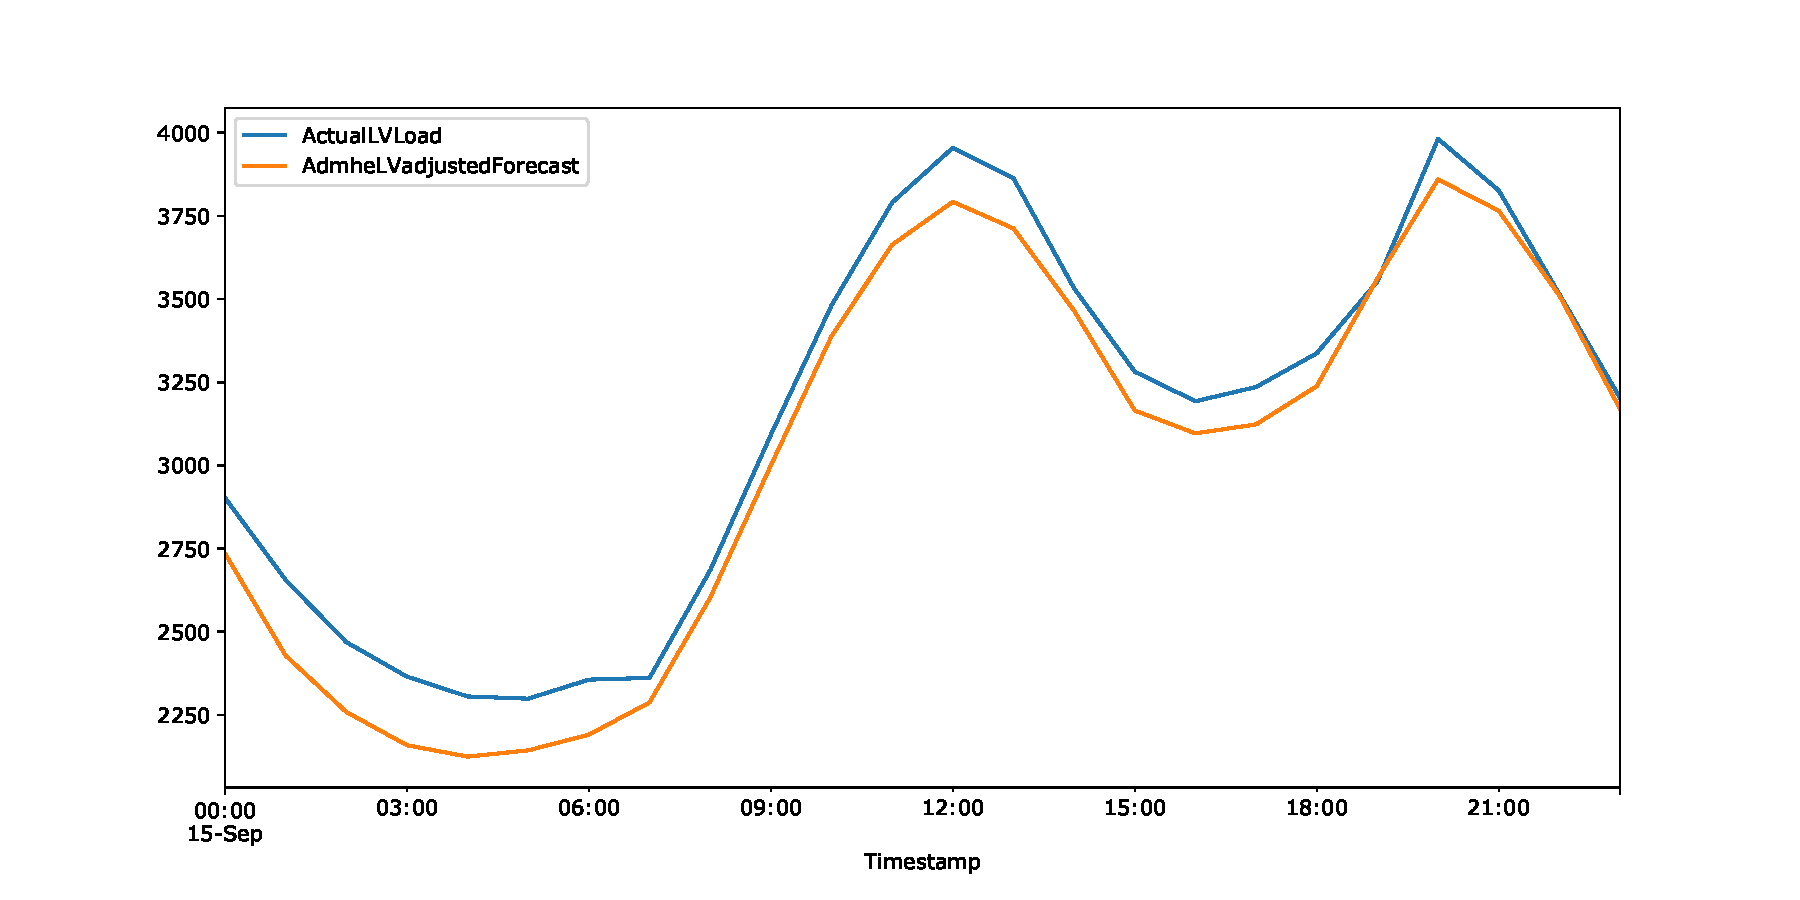
\includegraphics[width=1\linewidth]{project/loadadjustment.pdf}
\caption{ Actual LV VS OoEM's LV Adjusted Forecast}

\end{figure}
\par So to sum up the aim of this thesis is to create a model for daily Low Voltage load demand, which is not available by OoEM but the analysts have to declare it nonetheless. The above described algorithm will be used in order to adjust OoEM's daily forecast for the whole network to the LV load forecast, as if OoEM provided on daily basis load demand forecast, and incorporate this information in the daily task of Low Voltage demand forecasting in our model's later.
\subsection{Outliers-Missing Values}
Having in mind that the datasets are certified load demand data and moreover that the IPTO's dataset presents the actual load demannd, we don't expect to have outliers, missing values or bad data  etc. The only case where we have to deal with "missing values" is on the Daylight saving time (DST) days. Daylight Saving Time is the procedure of setting the clocks forward one hour from standard time during the summer months, and back again in the fall, in order to make better use of natural daylight. This phenomenon is depicted in hour dataset as follows: Once a year there is a day with "23 hours" and also 23 hourly load demand values when local time is about to reach e.g Sunday, 31 March 2019, 03:00:00 clocks are turned forward 1 hour to
Sunday, 31 March 2019, 04:00:00 local daylight time instead. On the other hand, there is one day with 25 hours and 25 load demand values when the local daylight time was about to reach e.g Sunday, 27 October 2019, 04:00:00 clocks are turned backward 1 hour to Sunday, 27 October 2019, 03:00:00 local standard time instead. To deal with this situation, after communicatiing with an energy analyst, working for one of the biggest energy providers in Greece, we will fill the missing values with the previous' hour load demand and in the case of the extra hour, we will calculate the average load demand value for these two hours that the hour change occurs e.g in hour example, on 31 March we will take the average load demand of hours 3 and 4.
\subsection{Summary Statistics \& Data Visualizations}
Any data science problem, starts with the investigation of the available data to examine their properties and identify underlying correlations, so some exploratory data analysis was done on our dataset to this end. As we mentioned earlier, daily electricity load demand is greatly affected by seasonality, Holiday etc. In this task, our response variable is the LV e.g the load demand for load meters in hourly basis. In the following graphs, we will plot our response variable LV in order to identify interaction with time itself, as we are dealing here with time series, but also we will examine our variable of interest for any correlation with the rest of the explanatory variables. In the following graph, we can observe that Low Voltage load demand is a bit lower in Holiday, in contrary with normal days. This is fairly logical, because under the category of Low Voltage meters exist home meters, SME meters, office meters etc, so it is expected on Holiday when offices and SMEs are closed to expect lower load demand.
\begin{figure}[ht!]
\centering
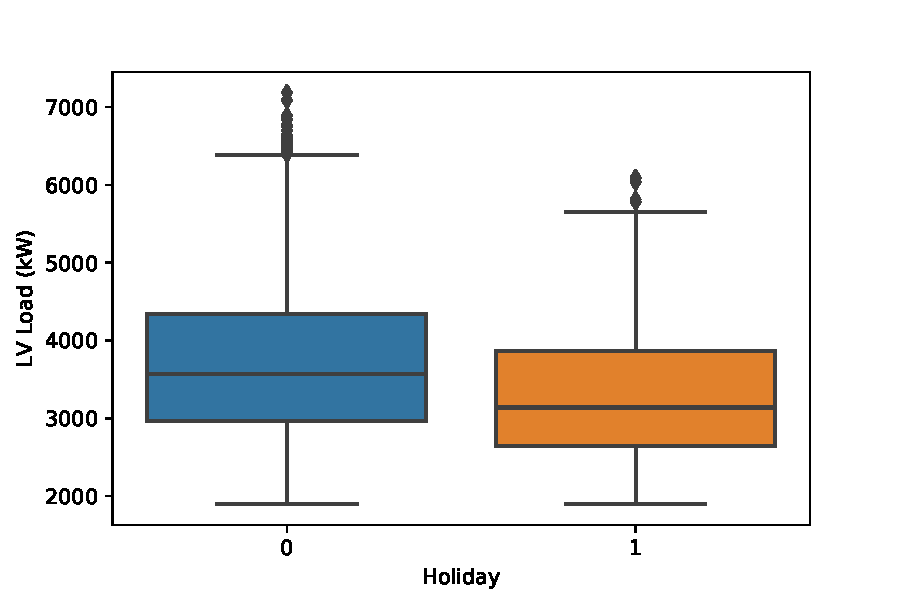
\includegraphics[width=0.75\linewidth]{project/eda1.pdf}

\caption{Low Voltage Load Demand vs Holiday}
\end{figure}
\par In the next graph, we plot the Low Voltage load demand based on the Weekday, e.g Monday, Tuesday...etc, in order to identify if and how the Weekday under examination affects the load demand. By observing the plot,we can infer that electric load demand is significantly lower during the Weekend because of reduced economic activity, as SMEs and offices are closed. Lower levels of demand are also observed on Mondays compared to the other "normal" - e.g non Holiday and non Weekend - days of the week, due to inertia caused by the reduced economic activity of Weekend.
\begin{figure}[ht!]
\centering
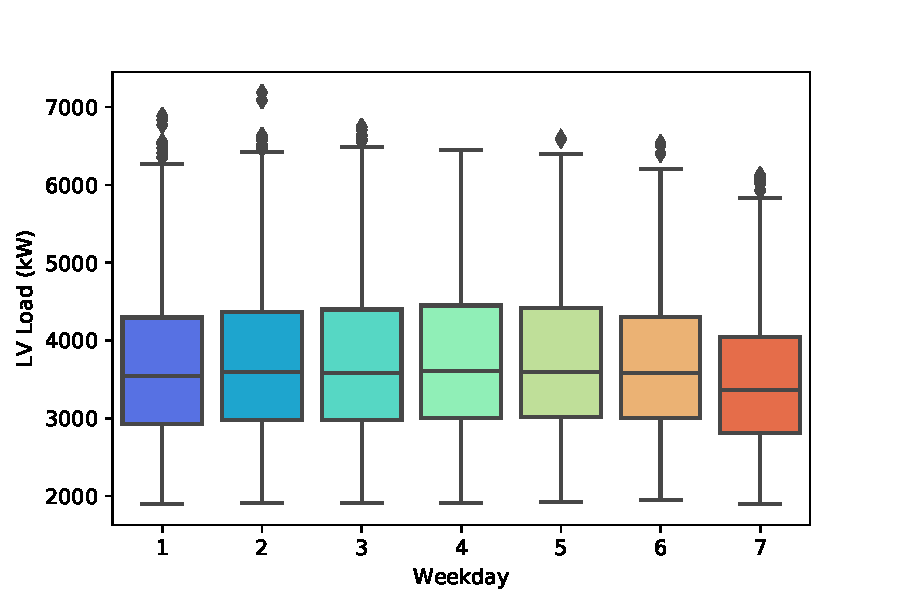
\includegraphics[width=0.75\linewidth]{project/eda2.pdf}

\caption{Low Voltage Load Demand vs Weekday}
\end{figure}
Here we create a boxplot for our response variable and we can observe that Low Voltage load demand most of the times, or in other words in the 2nd and 3rd quantile is approximately between 2800 and 4500 KWh, but as we can see there are values below 2000 KWh and also outliers over 6500 KWh per hour.
\begin{figure}[ht!]
\centering
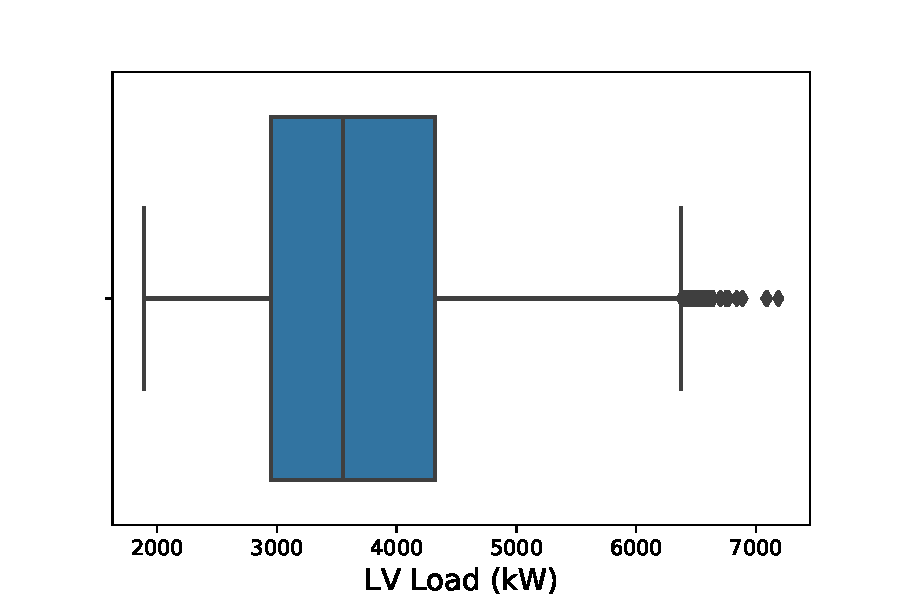
\includegraphics[width=0.7\linewidth]{project/eda3.pdf}

\caption{Low Voltage Load Demand Boxplot}
\end{figure}
Electricity load demand presents fluctuations during the course of the day, based on daily human activity. Given that our dataset contains hourly electric load demand values, which show diurnal variation in electric load demand. In the next graph, we plotted the low voltage load demand on a random day and as we can see, the hourly variation during the 24 hour period is evident. More specifically, we can observe that the first load demand maximum value appears close to midday due to extensive use of electricity both for household activities (e.g cooking, heating etc) and businesses activities (office lighting, PC usage etc) during the working hours. The second load demand maximum is observed during the late afternoon and early evening hours and this is due to the extensive use of lighting and heating or cooling.
\begin{figure}[ht!]
\centering
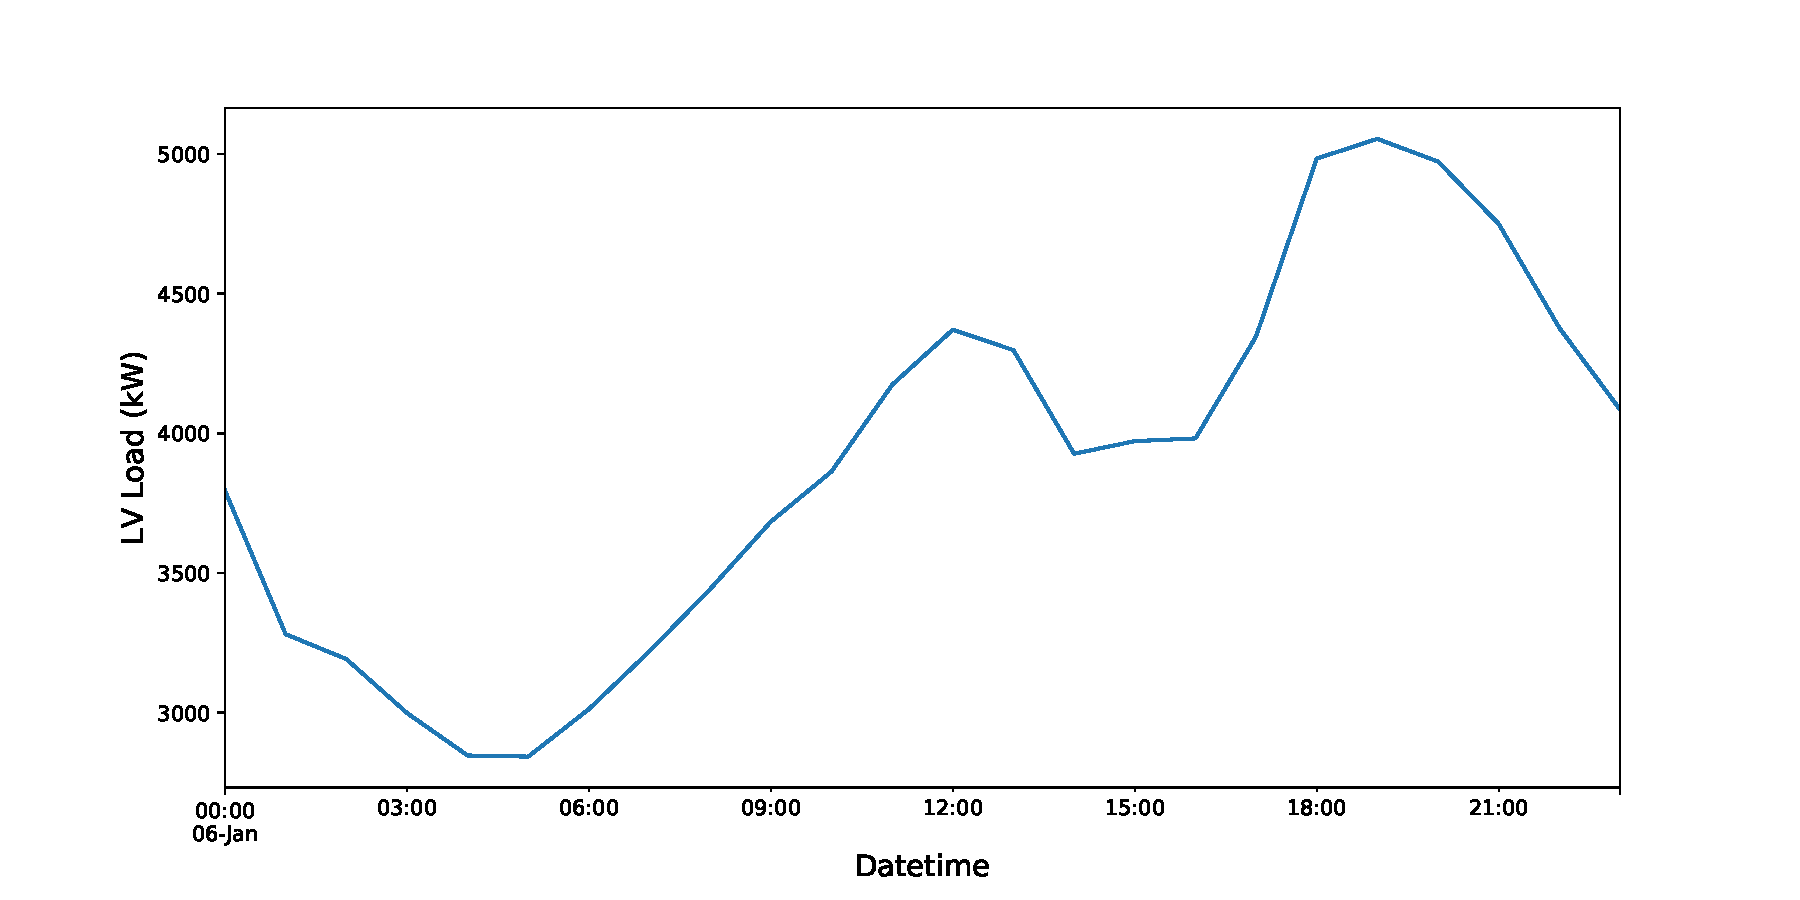
\includegraphics[width=1\linewidth]{project/eda4.pdf}

\caption{Daily Low Voltage Load Demand per Hour}
\end{figure}
\par In literature, there is a lot of discussion concerning electricity load demand and seasonality, thus we plotted the Low voltage load demand over one year time. More specifically, we used the actual LV load demand data of 2018 and plotted them over time. By looking at our graph, we can easily identify the strong seasonality appeared in the electric load demand behaviour, where there is observed higher load demand in winter in contrary with the summer. More specifically, we can observe higher electricity load demand in January, which thereafter gradually decreases until May. The above mentioned decrease in demand, moving towards the Spring as the weather gets warmer, coincides with a decrease in demand for heating.  As we move into the Summer, we observe a gradual increase in electricity demand, due to extensive use of air conditioners as the temperature gets higher and higher. This trend continues throughout the period of Summer till September, with the exception of August when a significant decrease in load demand is obvious. This decrease in August can be explained by the fact that the majority of people is on summer vacation during this month. A slight decrease in electricity load demand is also observed in October, which is representative of the transition from summer to winter, just before starting to gradually increase again in the following months to reach a maximum in December. The electricity load demand in December is higher than in January and February (which are Winter's coldest months), due to increased load demand during the festive Christmas period. 
\begin{figure}[htbp]
\centering
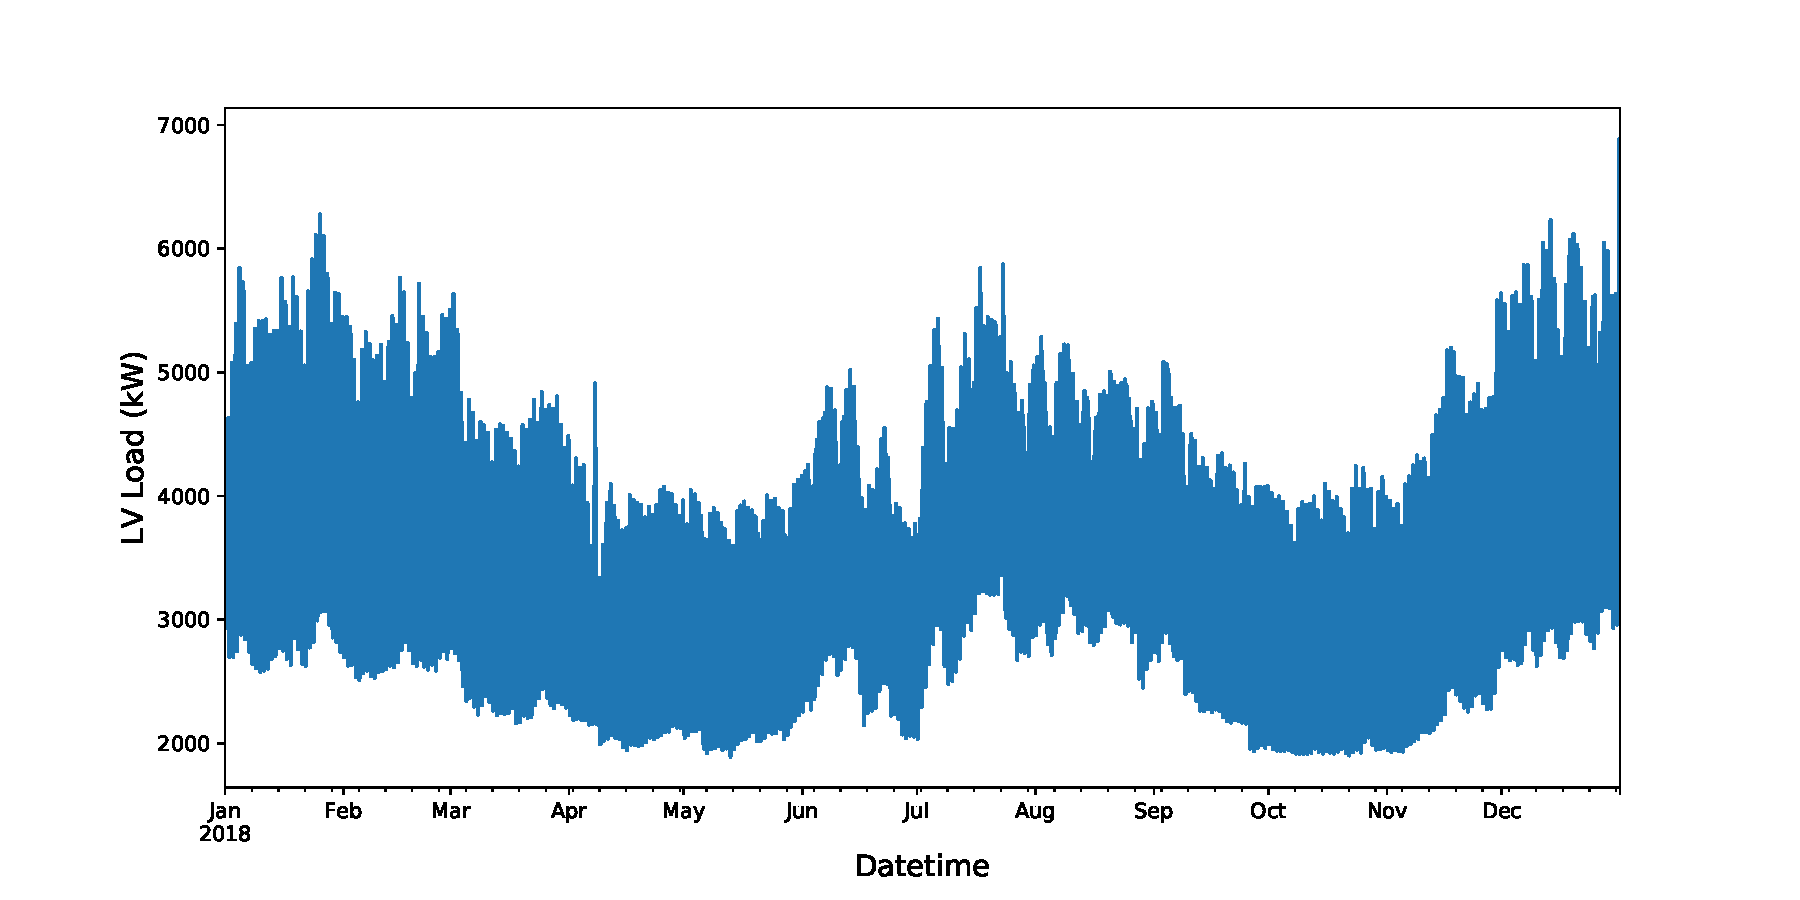
\includegraphics[width=1\linewidth]{project/eda5.pdf}

\caption{2018 Low Voltage Load Demand (Historical Data)}
\end{figure}
\par So from our exploratory analysis we can conclude the following:
\begin{itemize}
    \item Electricity load demand curve is seasonal and presents fluctuations across the week and throughout the day.
    \item Irregular events (e.g extreme weather) can heavily affect electric load demand.
    \item Seasonal trends and fluctuations observed in load curve are due to weather conditions or factors such as weekend and holiday effects.
    \item Load demand minimum values are observed in the transient seasons (Spring \& Autumn), whereas load demand maximum values are observed in Winter and Summer months.
    \item Lower electric load demand values are observed during holiday and weekends, in contrary with the normal weekdays (working days).
   \item  Last but not least, concerning daily variation, we observed that there is higher load demand during midday and late afternoon, regardless of season.
\end{itemize}
\newpage
\section{SARIMAX Model}
Fistly, we will apply the SARIMAX model and try to forecast Low Voltage load demand one day ahead, or in other words for the next 24 hours. As observed in the exploratory data analysis, there is trend and seasonality in our response variable and also our response variable is heavily affected by exogenous variables such Weekday, Holiday etc, so concerning ARIMA models, we will use the  Seasonal AutoRegressive Integrated Moving Average with eXogenous factor (SARIMAX (p, d, q)(P, D, Q, m)). To obtain the optimal order values, we used Python's \textit{auto arima()} \cite{autoarima} function with m=24, where m is the period for seasonal differencing and refers to the number of periods in each season, thus because we have hourly frequency in our time series we set it to 24. The auto arima function returned us the following optimal values for the SARIMAX orders as seen in the following figure.
\begin{figure}[ht!]
\centering
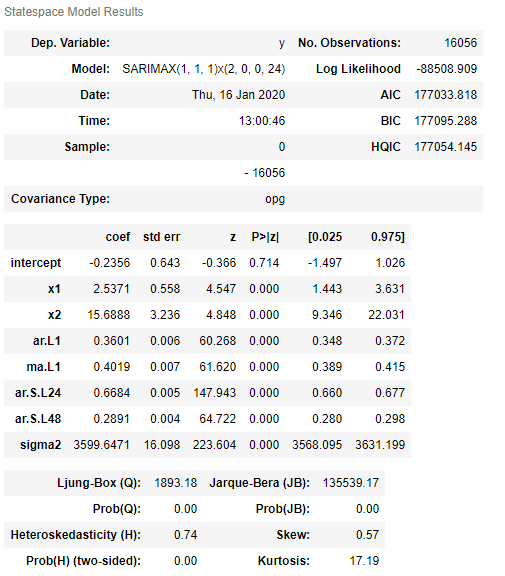
\includegraphics[width=0.5\linewidth]{project/modelsum.PNG}
\caption{SARIMAX optimal model summary}

\end{figure}
After obtaining the optimal values (\textbf{SARIMAX(1,1,1)x(2,0,0,24)}) from the function we split the dataset into train and test set, where the test set is the dataset's last day or in other words the last 24 hours that we want to predict. Then we fit a SARIMAX model with the appropriate order values and the Holiday and Weekend variables as exogenous factors. After fitting the model we will make the predictions and in order to evaluate the model we will use the Root Mean Square Error metric.
As said earlier, the object of this thesis is to create a model that we be more accurate than the OoEM's forecast model, thus every forecast will be compared with that forecast which is the value that we created earlier LVForecastEstimation. Again we should note that the LVForecastEstimation is the best case scenario, because OoEM does not know a-priori the proportion of Low Voltage in his daily total load forecasts. We were able to calculate this percentage based on historical data with one month lag as mentioned earlier. 
In the following figure, we plotted our result to get a graphical representation of our model's accuracy where the blue line \textbf{LV}, is the dataset's actual LV load demand as calculated earlier, the green line \textbf{LVForecastEstimation} is the OoEM's forecast LV load demand as calculated earlier and the orange line \textbf{OurPrediction} is the SARIMAX model's predicted values.
\begin{figure}[ht!]
\centering
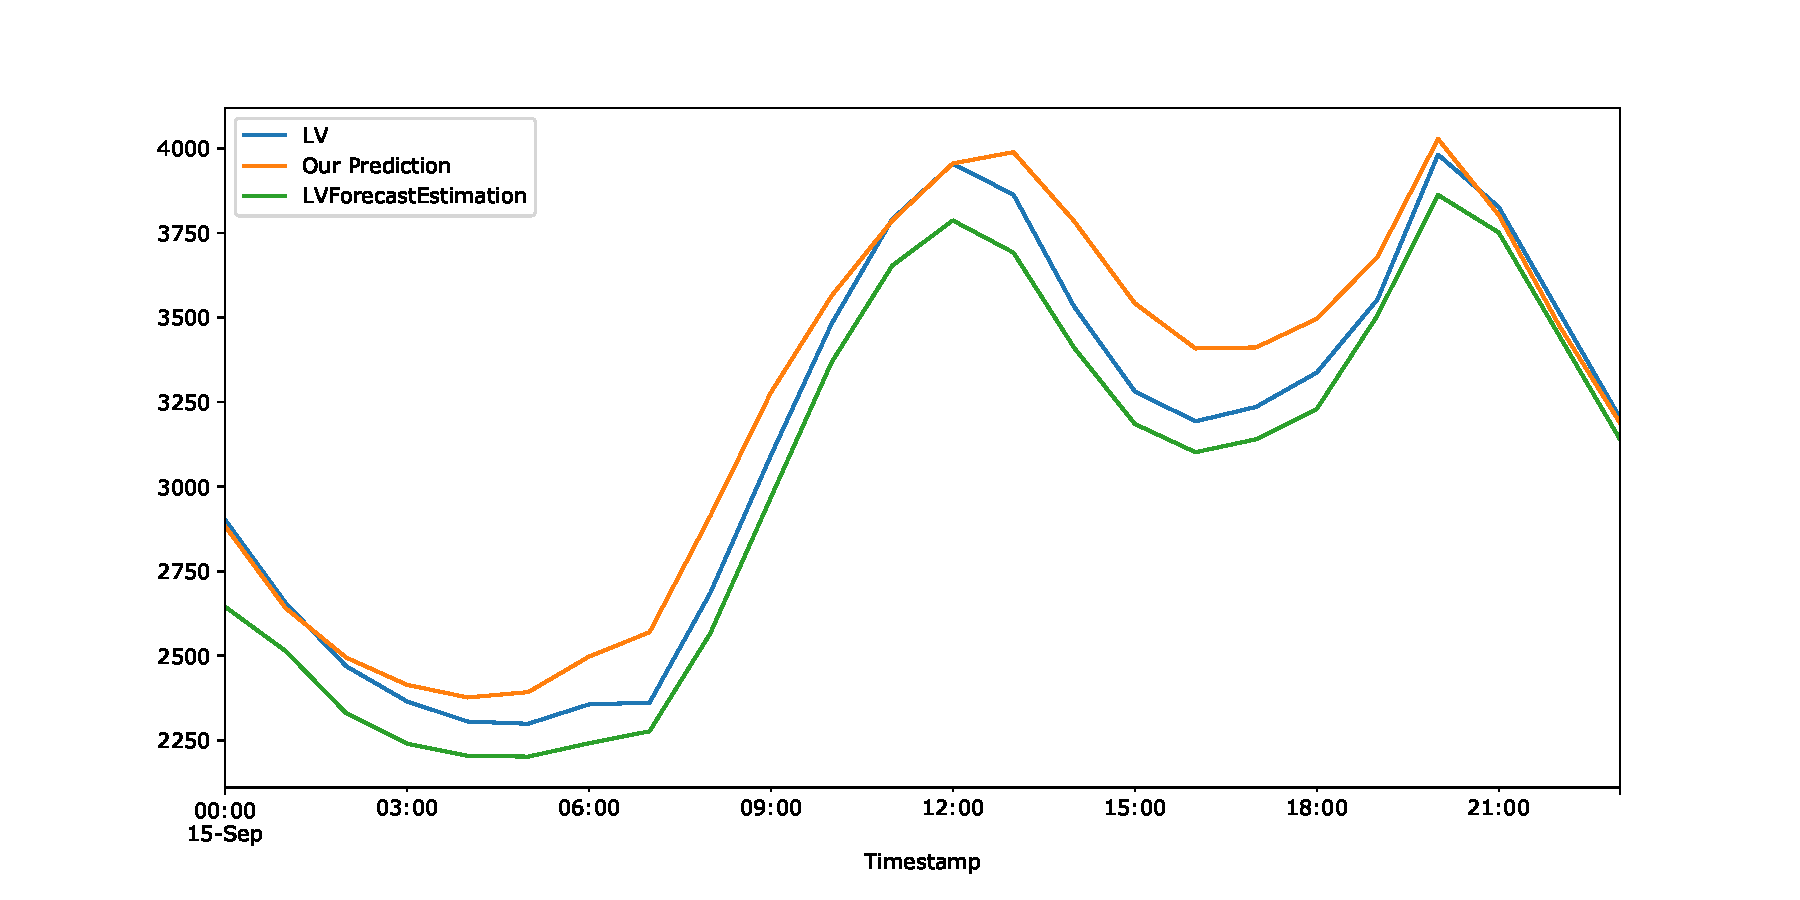
\includegraphics[width=1\linewidth]{project/sarimax.pdf}
\caption{SARIMAX LV load forecasts vs Actual load vs OoEM's load forecast}
\end{figure}
\par By looking at the graph, we can conclude that our prediction is very decent, because as we can see the model follows very accurately the daily seasonality, although the OoEM's forecast is slightly better. In order to quantify the error, we will use the RMSE error as we said earlier and calculate our's prediction RMSE and the OoEM's prediction RMSE, as seen on the table below.
\begin{table}[ht!]
\centering
\begin{tabular}{lllll}
\cline{1-2}
\multicolumn{1}{|l|}{\textbf{Their RMSE Error}} & \multicolumn{1}{l|}{\textbf{Our RMSE Error}} &  &  &  \\ \cline{1-2}
\multicolumn{1}{|c|}{\textit{123.23}} & \multicolumn{1}{c|}{\textit{136.03}} &  &  &  \\ \cline{1-2}
                                &                                &  &  &  \\
                                &                                &  &  & 
\end{tabular}
\end{table}
\newpage 
\section{Prophet Model}
In this section, we will use Facebook's Prophet algorithm to make a forecast on the same day as before in order to be able to make the comparison between models easier. This time we will import and then use the Python's Prophet library, to create our Prophet model. This algorithm, requires some data preprocessing in order to work, as we mentioned earlier. Because we have holidays and weekday in our dataset that we would like to model as it affects load demand in a great way, we must create a dataframe for them, which should include the holiday occurrences and the weekday sequence, both in the past (historical data) and in the future (forecast horizon). Then again, we fit the Prophet model and then we will make a forecast again for the last 24 hours as before, and again in order to evaluate the model we will use the Root Mean Square Error metric. Furthermore, in order to produce even better forecasts, we tuned some of the model's parameters as seen below \cite{prophet}.
\begin{itemize}
    \item \textit{growth}: We set this parameter as "linear" because by observing our time-series plot we identified that there is a trend that keeps on growing with no real saturation insight. In any other case, e.g when the response variable must saturates, we would set this parameter to "logistic".
    \item \textit{holidays\_prior\_scale}: This parameter concerns the holiday effect on our time-series data. In other words, determines how much of an effect holidays should have on our predictions. When we know that holiday have a massive impact on our data, we should try large values. In our case after several tests, we set the holidays\_prior\_scale equal to 30.
    \item \textit{changepoint\_prior\_scale}: This parameter indicates the changepoints flexibility value. Here large values denotes more flexiblity in the model, although you may end up overfitting. Several tests made and we found the optimal changepoint\_prior\_scale value to be 50.
    \item \textit{seasonality\_mode}: This parameter illustrates the way that seasonality terms should be incorporated into the predictions. The availiable options here are additive or multiplicative. In general, when the forecasted measure is affected by seasonalities we should set this parameter to multiplicative. As we saw in our EDA, load demand is greatly affected by seasonality thus we will use multiplicative in order to strengthen the seasonality effect in our model's forecasting procedure.
    \item \textit{seasonality\_prior\_scale}: This parameter indicates the seasonality flexibility value. Again large values allow more seasonality flexibility in the model and after several tests we set the seasonality\_prior\_scale value equal to 50.
     \item \textit{yearly\_seasonality}: Indicates whether yearly seasonality is present on the data. We set this value to true, as observed in the EDA section.
     \item \textit{weekly\_seasonality}: Indicates whether weekly seasonality is present on the data. We set this value to true, as observed in the EDA section.
     \item \textit{daily\_seasonality}: Indicates whether daily seasonality is present on the data. We set this value to true, as observed in the EDA section.
\end{itemize}{}
Last but not least, to improve even more the model's forecasting ability, we added two additional regressors concerning the type of day e.g whether the day under study is Holiday or not and the day of week respectively. As we saw in the EDA part, these two independent variables affect in a massive way load demand, so we decided to incorporate them in our model as well. Both of these independent variables values must be known a-priori both in the past and in the future. According to literature, adding more regressors is crucial concerning accurate forecasting in Prophet algorithm, as it's a way to tune the model and make the forecasting procedure more clear and user-friendly.
\par To visualize individual forecast components, we used Prophet’s built-in plot\_components function: As we observe in the following component visualizations, Prophet was able to accurately model the underlying trend in the data, while also accurately modeling weekly,yearly and daily seasonality. The components plot consists of e sections: the trend, the extra regressors, and the seasonality. The sum of those components account for the entirety of the model in fact. The trend is simply what the data is showing if you subtract out all of the other components. The extra\_regressors plot shows the effect of all of the regressors (Weekday \& Holiday) included in the model. Additional regressors are like holidays in that they cause the trend to deviate from the baseline, except that the trend will stay changed after the event. The weekly seasonality component shows that load demand is constantly increasing throughout he week, but with a steep decline on the Monday. Moreover, the yearly and daily seasonality is quite wavy as can be observed in the plots. These plots are created with Fourier transforms, essentially stacked sine waves.
\begin{figure}[ht!]
\centering
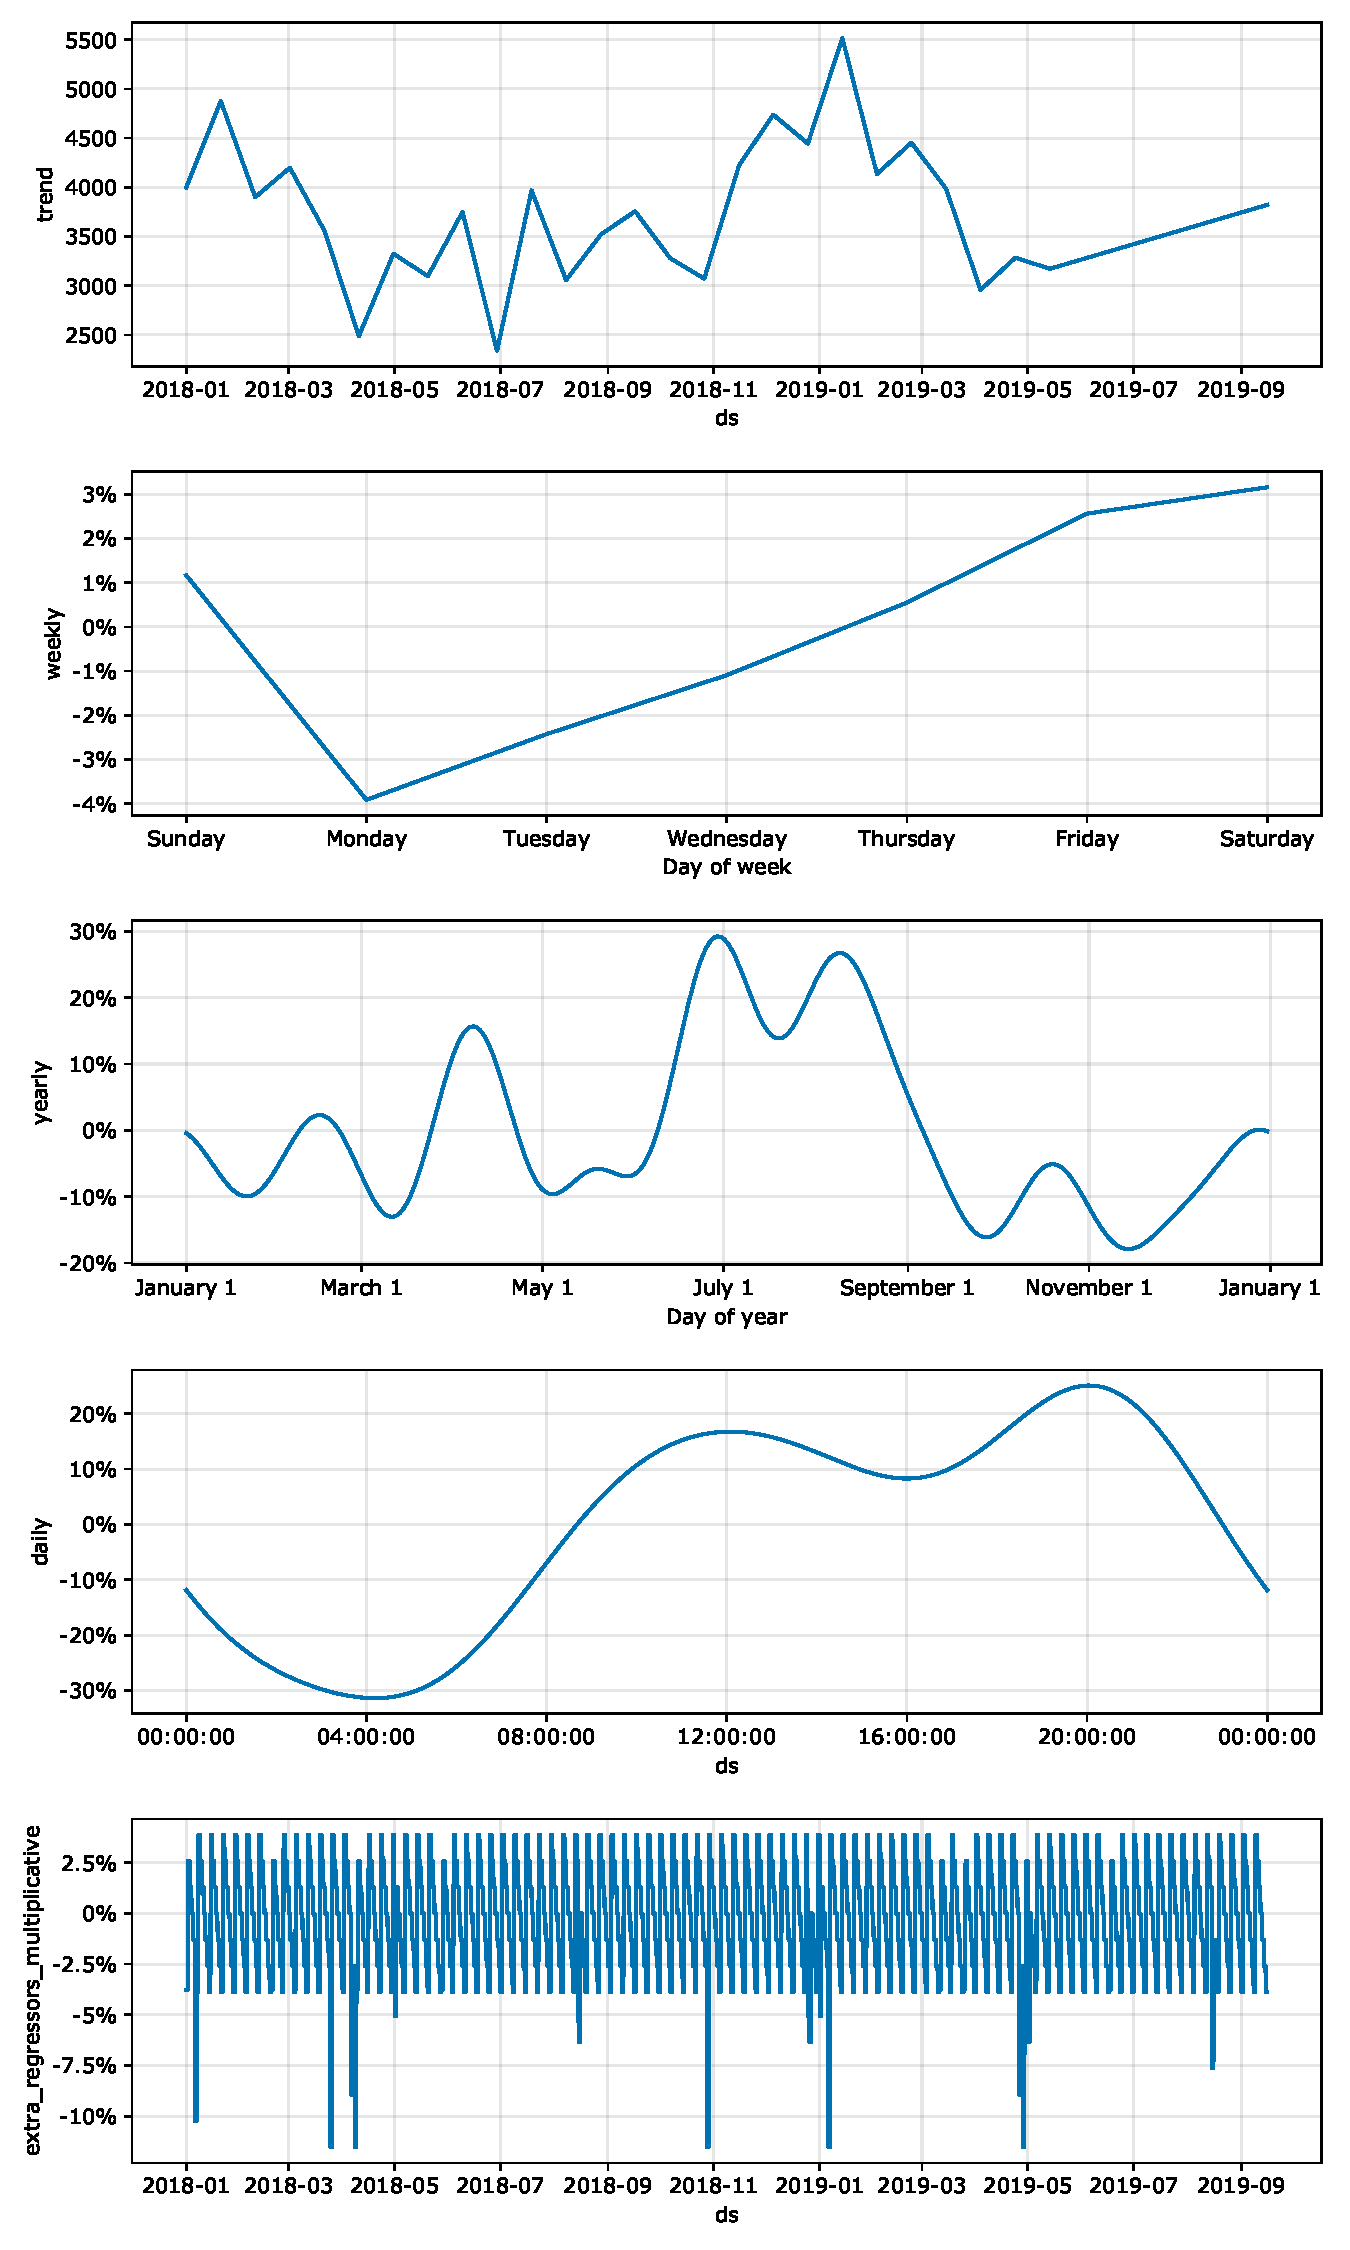
\includegraphics[width=0.7\linewidth]{project/download.pdf}

\caption{PROPHET's components}
\end{figure}
\newpage
Last but not least, after generating the forecasts using the Prophet model for the same day as before in order to be able to compare, we plotted our predictions.
In the following figure, we plotted our result to get a graphical representation of Prophet model's accuracy where the blue line \textbf{LV}, is the dataset's actual LV load demand, the green line \textbf{LVForecastEstimation} is the OoEM's forecast LV load demand as calculated earlier and the orange line \textbf{OurPrediction} is the Prophet model's predicted values. 
\begin{figure}[ht!]
\centering
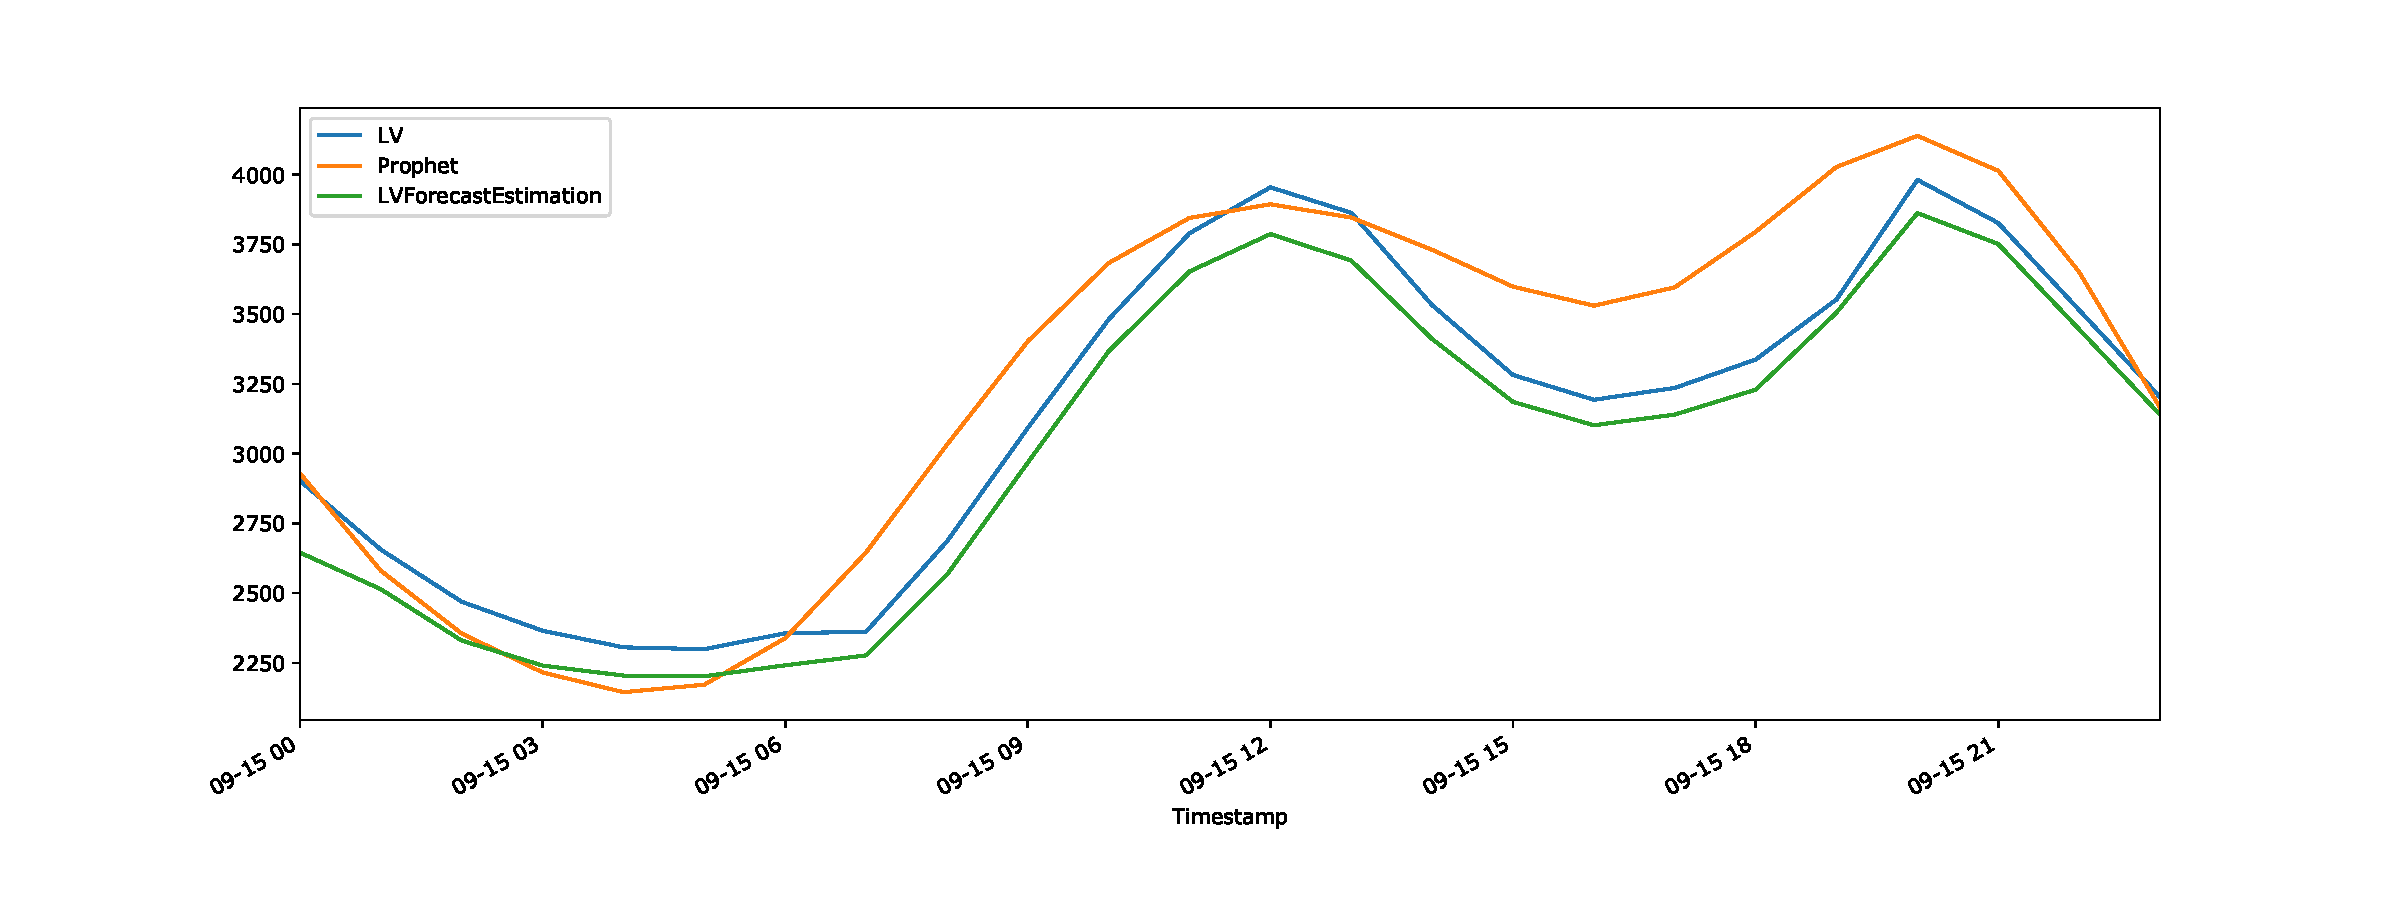
\includegraphics[width=1\linewidth]{project/prophet2.pdf}
\caption{PROPHET LV load forecasts vs Actual load vs OoEM's load forecast}
\end{figure}
By looking at the graph, we can clearly see that our prediction is not as good as before, and although the model seems to follow the daily seasonality the model is not accurate, and of course the OoEM's forecast is much better. Again to quantify the error, we will use the RMSE error as we said earlier and calculate our prediction's RMSE as seen on the table below.
\begin{table}[ht!]
\centering
\begin{tabular}{lllll}
\cline{1-2}
\multicolumn{1}{|l|}{\textbf{Their RMSE Error}} & \multicolumn{1}{l|}{\textbf{Our RMSE Error}} &  &  &  \\ \cline{1-2}
\multicolumn{1}{|c|}{\textit{123.23}} & \multicolumn{1}{c|}{\textit{235.20}} &  &  &  \\ \cline{1-2}
                                &                                &  &  &  \\
                                &                                &  &  & 
\end{tabular}
\end{table}
\newpage
\section{Multivariate Multi-Step LSTM Model}
In this section, we are going to investigate Neural Networks and we will create a special type of NN which is the LSTM neural network. As we saw earlier, we created an hourly observation of LV load demand based on the total network's actual values. Thus for each day, we will have 24 observations one for every hour of the day. Generally, in Deep Learning it is crucial to scale features before training a neural network. More specifically, before creating the model we have to do some data preprocessing, which involves framing the dataset as a supervised learning problem and normalizing the neural network's input variables. Concerning the continuous variables we will use Python's function MinMaxScaler() to do the scaling \cite{mckinney2012python}, whereas for the categorical variables we will use One-Hot-Encoding. After doing the scaling of the data, we will split it in train/test dataset and we will use the 33\% of the dataset as test dataset \cite{keras}. 
\par In a multi-step prediction model, based on the past history values (whose length in the past is defined by the user), the model is asked to predict a range of future values. 
In other words, the multi-step neural network model needs to learn to predict a predict a sequence of values in the future, in contrary with a single-step neural network model, where only a single future point is predicted. The above mentioned framing of the problem is also known as a multi-step time series forecasting problem, given the multiple forecast steps and furthermore a model that uses multiple input variables is scientifically called a multivariate multi-step time series forecasting model, which this is our case-study in this experiment. For the multi-step model, after doing some experiments we chose the training data to consist of hourly load demand observations over the past fifteen days \cite{kong2017short}. Thus, we have to create a time window containing the most recent 288 (15x24) observations to train our neural network model. These time intervals from now on will be called windows, and there are the windows of time containing the appropriate data for the model to train on. The window \textit{past history} denotes the size of the past window of data observations, whereas the \textit{target size} denotes how far in the future the model need to learn to predict. Here according to the business rules, the model needs to learn to predict the load demand value for the next day. Since an obversation is recorded every hour, the output consists of 24 predictions e.g one for every hour of the day. 
\par 
As mentioned earlier, the dataset needs to be prepared accordingly before training, thus the first step is just to re-create it, but this time with the appropriate pre-specified \textit{past history} and \textit{target size}. Concerning the LSTM neural network architecture, we used Keras library \cite{keras} and after doing some experiments, we concluded in creating a sequential model with 4 Layers. The first and the second layer have 100 LSTM neurons each, whereas the third one has 50 neurons. The last layer, is a Dense layer and since 24 predictions are made (forecasting 24 hours in the future ), the dense layer has 24 neurons. 
\begin{figure}[ht!]
\centering
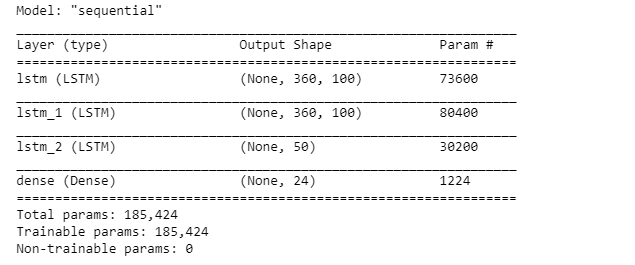
\includegraphics[width=0.8\linewidth]{project/lstmsummary.PNG}
\caption{Multi-Variate \& Multi-Step LSTM Model Summary}
\end{figure}
The model was trained for 20 epochs with a batch size of 256 and concerning the loss function we used the Root Mean Square Error (RMSE) and the Adam optimiser also. The Adam optimization algorithm is described in literature as an extension of the stochastic gradient descent algorithm and recently has seen broader adoption in the scientific community concerning neural network applications.  Adam optimization algorithm or Adam optimizer is used in neural networks to update network weights in an iterative way based on the training data. In the next plot, we present our neural networks training and validation loss curves, that were extracted after finishing with the training of our model.
\begin{figure}[ht!]
\centering
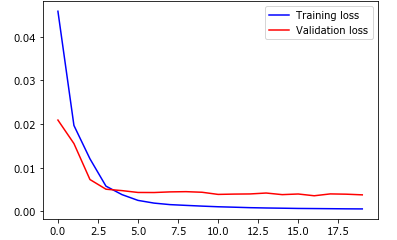
\includegraphics[width=0.7\linewidth]{project/tl.png}
\caption{LSTM Model's Train \& Validation Loss}
\end{figure}
\par To evaluate how well our neural network learnt to predict the future, a \textbf{rolling-forecast} scenario will be used, which is also technically described as walk-forward model validation. In simple words, each time step of the test dataset will be walked one observation at a time. More specifically, the proposed neural network model will make a forecast for a specific time step and then, after the forecast, the actual expected load demand value for the next time step of the test dataset will become available to the neural network in order to be incorporated in the forecast for the load demand value of the next time step, e.g the load demand value for the next hour. In other words, when the neural network model is required to make a 24 hour forecast in the future, then after the forecast, the actual load demand data for that 24 hour period is made available to the neural network model, in order to be used for making a forecast on the subsequent 24 hour period. The above described procedure is realistic concerning the way that the model will be used in practice and also beneficial, by allowing the neural network model to use the most recent available data. After making the forecasts and obtaining the predicted values, we have to invert the data transformations made earlier, in order to return the predicted load demand values back into their original scale. We can do this directly, using Python's \textit{MinMaxScaler} object that offers an inverse transformation function (\textit{invert\_transformation()} ). All collected forecasts made on the same test dataset and then we implemented an error score function - which used once again the RMSE metric - in order to summarize the model's forecasting skill (for each time step) and output an average of all the prediction errors. 
\par Furthermore, in the following figure, we plotted our result to get a graphical representation of our model's accuracy where the blue line is the \textbf{past history}, e.g the dataset's actual LV load demand for the declared history size window -in our case 15 days of previous observations-, the green line is the \textbf{true future}, the current actual LV load demand for the specified target size e.g how far in the future does the model need to learn to predict. Last but not least, the red line \textbf{Predicted Future} is the predicted values forecasted by the LSTM Neural Network for the specified target window size e.g 24 hours in the future based on the specified past history window size e.g using 15 days history data to make the prediction \cite{tensor}. 
By looking at the graph, we can clearly see that our prediction is again worse than before, and although the model seems to recognise the hourly seasonality -as it is denoted by the spikes and the ups and downs in the graph- but the model is not accurate enough. To quantify the error, we will use the RMSE error as we said earlier and calculate our prediction's RMSE as seen on the table below. As we can see once again, the OoEM's forecast is still better.
\begin{figure}[ht!]
\centering
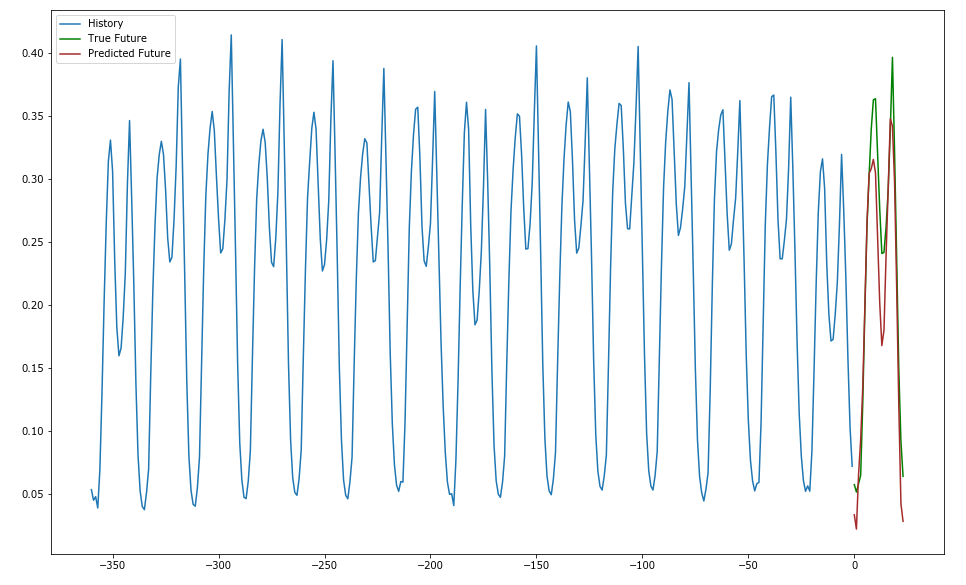
\includegraphics[width=0.9\linewidth]{project/nn.PNG}
\caption{LSTM model's load forecasts vs Actual Load}
\end{figure}
\begin{table}[ht!]
\centering
\begin{tabular}{lllll}
\cline{1-2}
\multicolumn{1}{|l|}{\textbf{Their RMSE Error}} & \multicolumn{1}{l|}{\textbf{Our RMSE Error}} &  &  &  \\ \cline{1-2}
\multicolumn{1}{|c|}{\textit{123.23}} & \multicolumn{1}{c|}{\textit{194.10}} &  &  &  \\ \cline{1-2}
                                &                                &  &  &  \\
                                &                                &  &  & 
\end{tabular}
\end{table}
\newpage
\section{Time Series as a Regression Problem}
As we mentioned earlier, in literature there are numerous publications concerning Electricity Load Demand Forecasting, which state that this forecasting problem should be approached as a regression problem and as confirmed in the EDA section, there are numerous exogenous factors that affect load demand and also it's affected greatly by seasonality. Thus in this section, we will try to approach this problem as a regression problem, we will apply some of the state-of-the art algorithms and evaluate their performance. To do that first of all, we have to make some transformation in our dataset. First of all we will create four more columns, which will denote the Day, Hour, Month and Year of the observation respectively. Moreover as we saw, earlier the LV load demand presents apart from great seasonality, indicates autocorrelation also \cite{vanderplas2016python}. \textbf{Autocorrelation} metric is used to measures the linear relationship between lagged values of a time series, just as correlation metric used to estimate the extent of linear relationship between two variables, by identifying and measuring their interaction. In other words, autocorrelation phenomenon occurs when time-series is linearly related to a lagged version of itself.
\par The estimation of this linear relationship between lagged values is realized by the \textbf{Autocorrelation coefficients}, as shown in the following formula. More specifically, $r_{1}$ measures the linear relationship between lagged values $y_{t}$ and $y_{t-1}$, $r_{2}$ measures the linear relationship between lagged values $y_{t}$ and $y_{t-2}$ and so on and so forth. The value of $r_{k}$ can be formulated as
\begin{figure}[ht!]
\centering
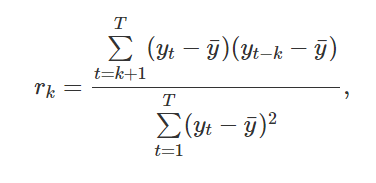
\includegraphics[width=0.6\linewidth]{project/rk.PNG}

\end{figure}
where T is the time series length. When time-series have trend, the autocorrelation value for small lag intervals tend to be large and positive, because nearby observations in terms of lag intervals, tend to be similar in size and small discrepancies are observed. Autocorrelation plots of time-series which have trend, present large positive autocorrelation values that slowly decrease as the lags time intervals gets bigger. 
On the other hand, when seasonality is observed in the time-series, autocorrelations will be larger for the seasonal lag intervals (multiples of the seasonal frequency). In cases such electric load curve when data present both trend and seasonality, a combination of these effects is observeved as shown in the following plot. In the next graph, we present the autocorrelation plot of our response variable, e.g the LV load demand. 
\begin{figure}[ht!]
\centering
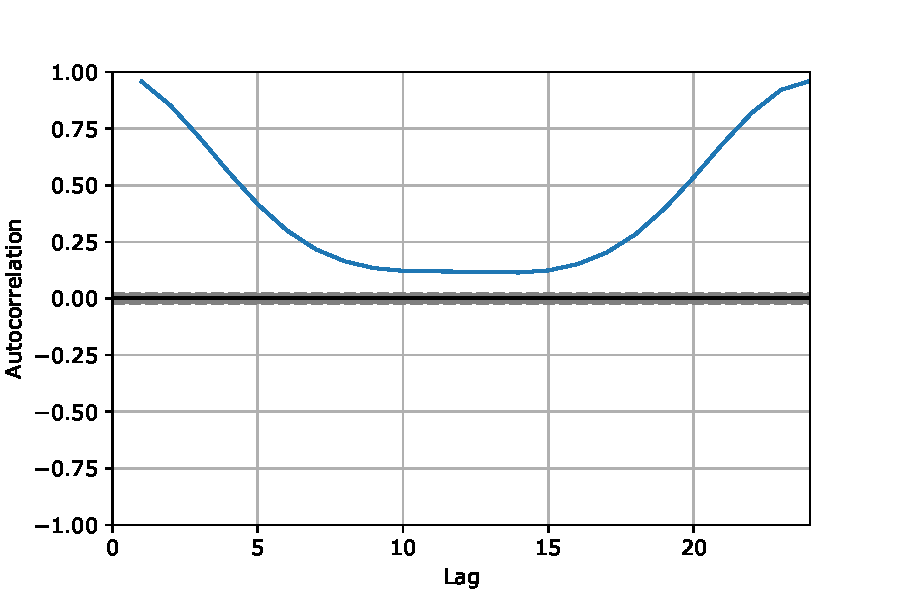
\includegraphics[width=0.6\linewidth]{project/ac.pdf}

\caption{Auto-correlation plot over 24 hour period}
\end{figure}
\par The autocorrelation plot below shows the extent to which the demand variable correlates with itself at different intervals (lags). This plot shows that demand is highly autocorrelated over the closest 6 hour period. To incorporate this information in our dataset, we created a function to generate for each observation in the dataset, the LV load demand value for closest 6 lags. Thus now our dataset contains the following columns, 
\begin{itemize}
    \item Year: The year that the load value is referring to.
    \item Month: The month that the load value is referring to.
    \item Hour: The hour (t) that the load value is referring to.
    \item Weekday: The day of Week (starting from Monday) that the date is referring to.
    \item Holiday: Indicator of whether this day is a Holiday or not.
    \item LV: The load demand for Low Voltage for that hour of the specific day.
    \item LV\_lag1: The load demand for Low Voltage on hour (t-1). 
    \item LV\_lag2: The load demand for Low Voltage on hour (t-2). 
    \item LV\_lag3: The load demand for Low Voltage on hour (t-3). 
    \item LV\_lag4: The load demand for Low Voltage on hour (t-4). 
    \item LV\_lag5: The load demand for Low Voltage on hour (t-5). 
    \item LV\_lag6: The load demand for Low Voltage on hour (t-6). 
\end{itemize}
as shown in the picture below.

\begin{table}[ht!]
\scalebox{0.7}{ 
\begin{tabular}{|c|c|c|c|c|c|c|c|c|c|c|c|c|}
\hline
\textbf{Timestamp}      & \textbf{Weekday} & \textbf{Holiday} & \textbf{Year} & \textbf{Month} & \textbf{Hour} & \textbf{LV} & \textbf{LV\_lag1} & \textbf{LV\_lag2} & \textbf{LV\_lag3} & \textbf{LV\_lag4} & \textbf{LV\_lag5} & \textbf{LV\_lag6} \\ \hline
\textbf{01-01-18 12:00} & 1                & 1                & 2018          & 1              & 12            & 4418.91     & 4384.56           & 4025.50           & 3575.72           & 3189.22           & 3048.66           & 2990.90           \\ \hline
\textbf{01-01-18 13:00} & 1                & 1                & 2018          & 1              & 13            & 4114.95     & 4418.91           & 4384.56           & 4025.50           & 3575.72           & 3189.22           & 3048.66           \\ \hline
\textbf{01-01-18 14:00} & 1                & 1                & 2018          & 1              & 14            & 3588.58     & 4114.95           & 4418.91           & 4384.56           & 4025.50           & 3575.72           & 3189.22           \\ \hline
\textbf{01-01-18 15:00} & 1                & 1                & 2018          & 1              & 15            & 3613.31     & 3588.58           & 4114.95           & 4418.91           & 4384.56           & 4025.50           & 3575.72           \\ \hline
\textbf{01-01-18 16:00} & 1                & 1                & 2018          & 1              & 16            & 3691.87     & 3613.31           & 3588.58           & 4114.95           & 4418.91           & 4384.56           & 4025.50           \\ \hline
\textbf{01-01-18 17:00} & 1                & 1                & 2018          & 1              & 17            & 4014.75     & 3691.87           & 3613.31           & 3588.58           & 4114.95           & 4418.91           & 4384.56           \\ \hline
\textbf{01-01-18 18:00} & 1                & 1                & 2018          & 1              & 18            & 4542.76     & 4014.75           & 3691.87           & 3613.31           & 3588.58           & 4114.95           & 4418.91           \\ \hline
\textbf{01-01-18 19:00} & 1                & 1                & 2018          & 1              & 19            & 4628.66     & 4542.76           & 4014.75           & 3691.87           & 3613.31           & 3588.58           & 4114.95           \\ \hline
\textbf{01-01-18 20:00} & 1                & 1                & 2018          & 1              & 20            & 4618.74     & 4628.66           & 4542.76           & 4014.75           & 3691.87           & 3613.31           & 3588.58           \\ \hline
\textbf{01-01-18 21:00} & 1                & 1                & 2018          & 1              & 21            & 4479.44     & 4618.74           & 4628.66           & 4542.76           & 4014.75           & 3691.87           & 3613.31           \\ \hline
\textbf{01-01-18 22:00} & 1                & 1                & 2018          & 1              & 22            & 4203.66     & 4479.44           & 4618.74           & 4628.66           & 4542.76           & 4014.75           & 3691.87           \\ \hline
\textbf{01-01-18 23:00} & 1                & 1                & 2018          & 1              & 23            & 3931.89     & 4203.66           & 4479.44           & 4618.74           & 4628.66           & 4542.76           & 4014.75           \\ \hline
\textbf{02-01-18 0:00}  & 2                & 0                & 2018          & 1              & 0             & 3490.90     & 3931.89           & 4203.66           & 4479.44           & 4618.74           & 4628.66           & 4542.76           \\ \hline
\textbf{02-01-18 1:00}  & 2                & 0                & 2018          & 1              & 1             & 3098.82     & 3490.90           & 3931.89           & 4203.66           & 4479.44           & 4618.74           & 4628.66           \\ \hline
\end{tabular}}
\end{table}



\par Then again, we are going to split the dataset in train/test datasets and apply one of the most state-of-the art algorithms for regression, LightGBM, to build our model and fit it. LightGBM Regressor is a Gradient Boosting Machine that has many parameters that can be tuned, thus we will use a technique called Grid Search in order to find the optimal parameters for our proposed model. Grid-searching is the process of scanning the data to configure optimal parameters for a given model, because certain parameters are necessary to be tuned depending on the algorithm that the model utilizes.  Grid-searching can be applied across machine learning to calculate the best parameters to use for any given model. During the process of Grid-Search, a model on each parameter combination possible will be built. The algorithm iterates through every possible parameter combination - among the values specified for each parameter- and stores the model for each combination. 
\newpage
\par So after running the GridSearch algorithm we reached a LightGBM Regressor model with the following parameters \cite{lightgbm}.
\begin{itemize}
    \item \textbf{boosting\_type: gbdt}
    \item \textbf{objective: regression}
    \item \textbf{num\_leaves: 1200}
    \item \textbf{learning\_rate: 0.17}
    \item \textbf{n\_estimators: 700}
    \item \textbf{max\_depth: 6}
    \item \textbf{metric: rmse}
    \item \textbf{bagging\_fraction: 0.8}
    \item \textbf{feature\_fraction: 0.8}
    \item \textbf{reg\_lambda: 0.9}
\end{itemize}

\begin{figure}[ht!]
\centering
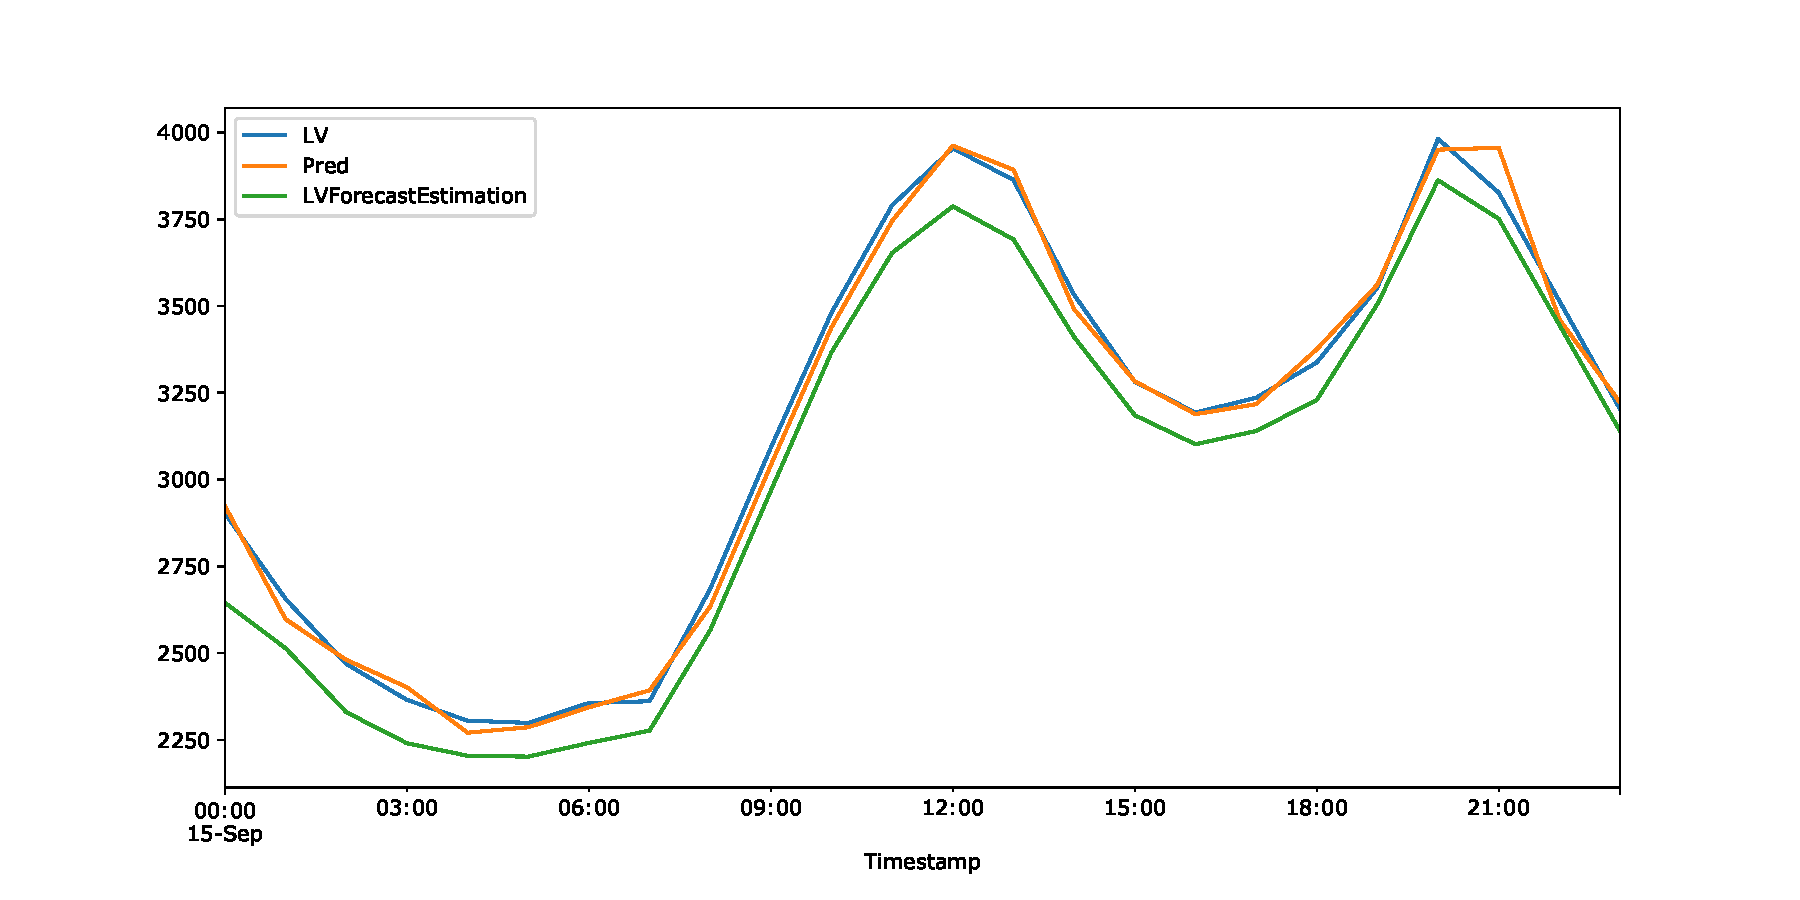
\includegraphics[width=1\linewidth]{project/final4.pdf}

\caption{LightGBM LV load forecasts vs Actual load vs OoEM’s load forecast}
\end{figure}
\begin{table}[ht!]
\centering
\begin{tabular}{lllll}
\cline{1-2}
\multicolumn{1}{|l|}{\textbf{Their RMSE Error}} & \multicolumn{1}{l|}{\textbf{Our RMSE Error}} &  &  &  \\ \cline{1-2}
\multicolumn{1}{|c|}{\textit{123.23}} & \multicolumn{1}{c|}{\textit{41.86}} &  &  &  \\ \cline{1-2}
                                &                                &  &  &  \\
                                &                                &  &  & 
\end{tabular}
\end{table}
\par As we can see in the provided graph our model generated great forecasts and even surpassed OoEM's forecast. Moreover, we used the RMSE error to quantify our results and we obtained a forecast with RMSE equal to 41.86 in contrary with OoEM's forecast which has an error of 123.23. Last but not least, to be even more confident about our model's general forecasting ability and also ensure that the above results were not random, we ran one more experiment as we tried to predict a whole month and more specifically the Semptember of 2019. Again we perform the same procedure, as we split the dataset in train and test sets and used the LightGBM model constructed above. Below we can see our results concerning the forecasting of one whole month. In the first figure, with the blue line are represented the actual Low Voltage load demand for September, where on the other hand with the orange line we present the evaluation criterion, or in other words OoEM's adjusted Low Voltage forecast.
\begin{figure}[ht!]
\centering
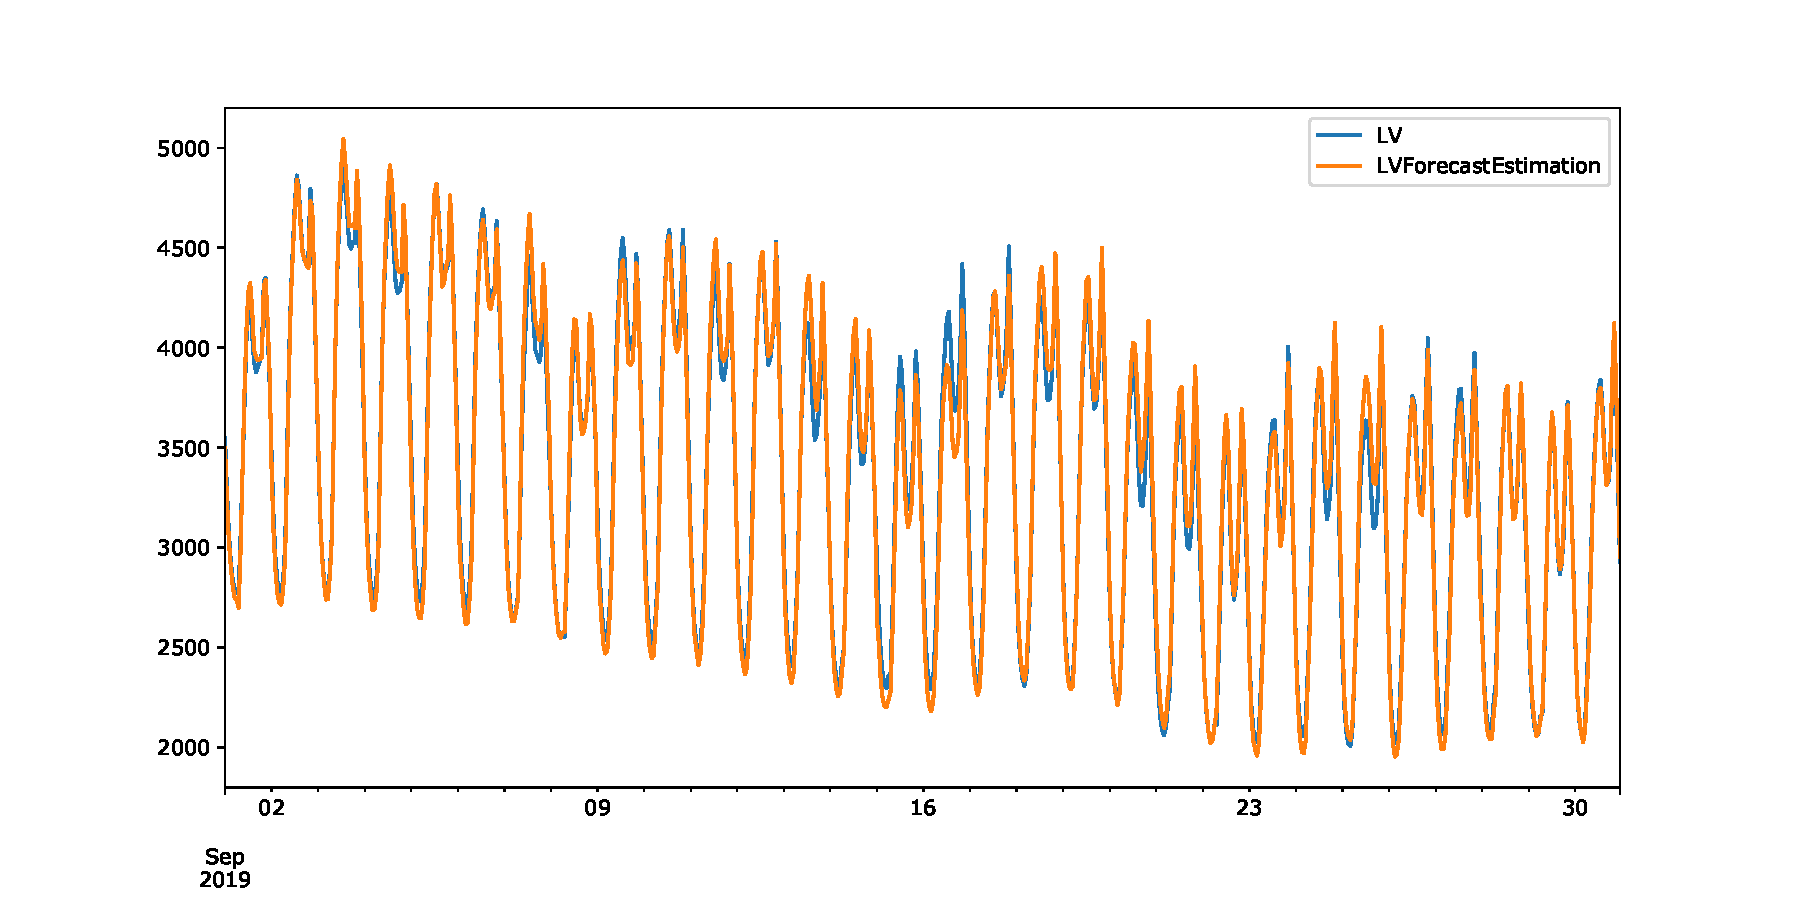
\includegraphics[width=1\linewidth]{project/1.pdf}
\caption{Actual LV load demand vs OoEM’s LV load forecast}

\end{figure}
In the second graph, with the blue line again we present the actual Low Voltage load demand for September, where on the other hand with the orange line we present our model's prediction for the Low Voltage load demand during September. By just looking at the two graphs, it's easy too understand that our model again performed better again and we quantified the error's again using RMSE which is our evaluation metric. The results are presented in the following table, where OoEM's forecast deviation where measured with an RMSE error of 88.14, where on the other hand our model generated an RMSE error of 55.73, thus outperforming OoEM's forecasts.
\begin{figure}[ht!]
\centering
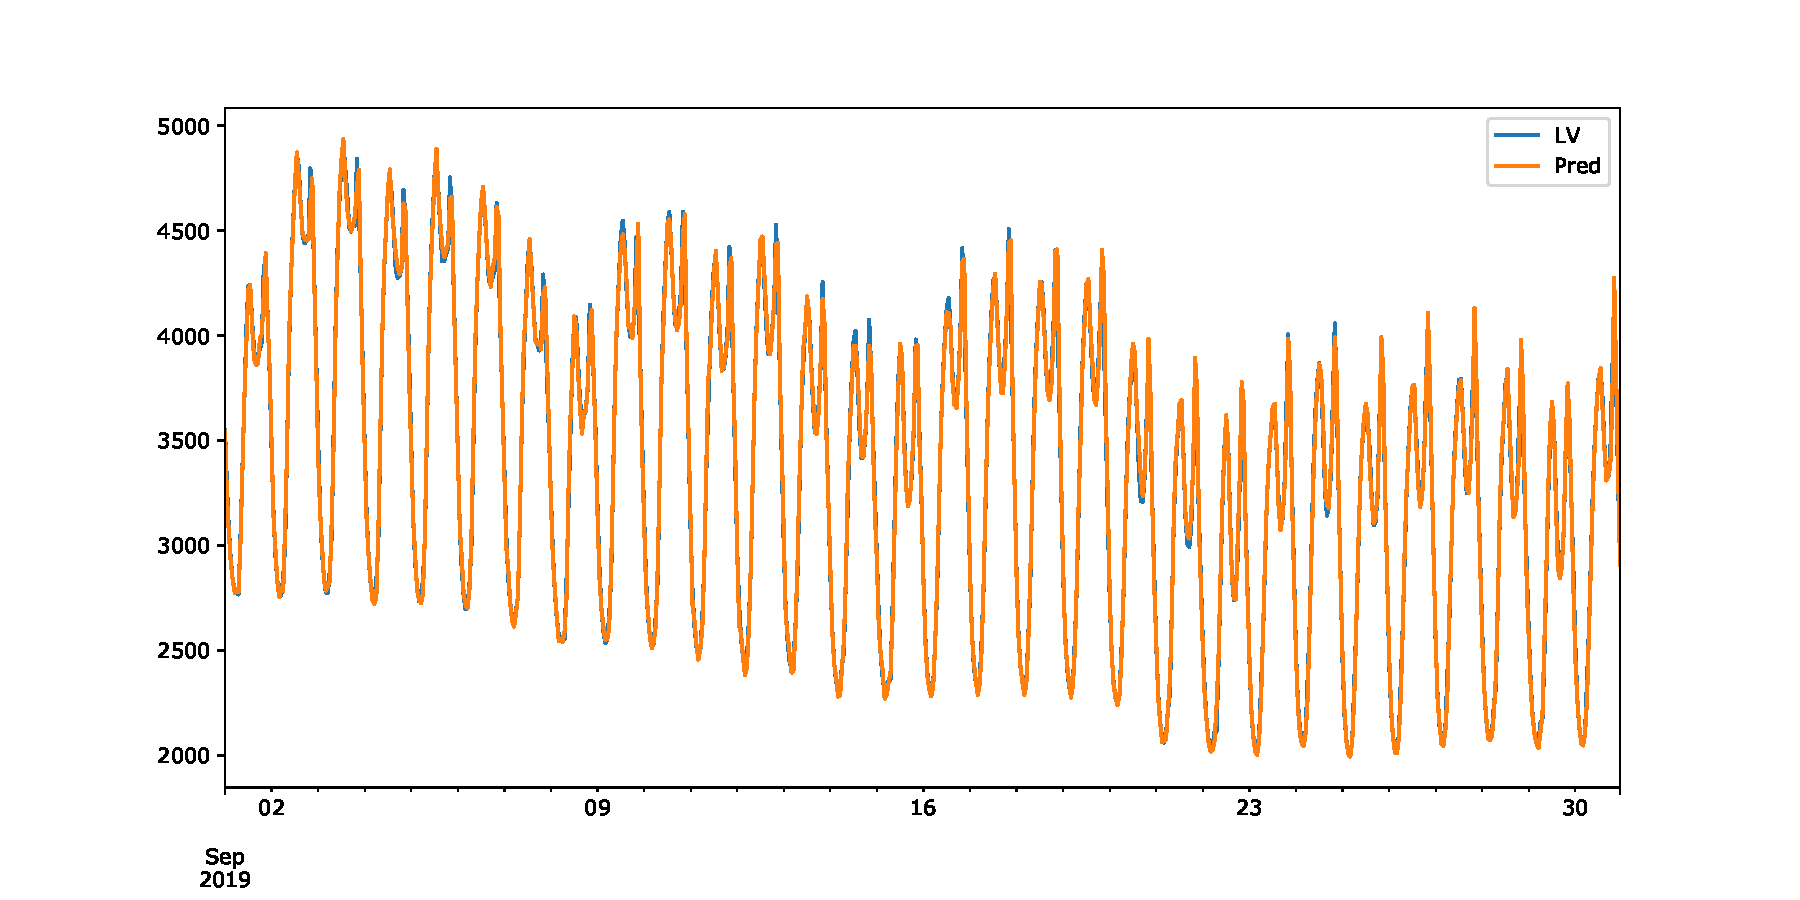
\includegraphics[width=1\linewidth]{project/2.pdf}
\caption{Actual LV load demand vs LightGBM model's LV load forecast}

\end{figure}
\begin{table}[ht!]
\centering
\begin{tabular}{lllll}
\cline{1-2}
\multicolumn{1}{|l|}{\textbf{Their RMSE Error}} & \multicolumn{1}{l|}{\textbf{Our RMSE Error}} &  &  &  \\ \cline{1-2}
\multicolumn{1}{|c|}{\textit{88.14}} & \multicolumn{1}{c|}{\textit{55.73}} &  &  &  \\ \cline{1-2}
                                &                                &  &  &  \\
                                &                                &  &  & 
\end{tabular}
\end{table}
Last but not least, to enhance our conclusion visually with greater detail, we provided graphs that visualize the forecast of three random days in September as forecasted by our models. In the following graphs, we present with the blue line the actual Low Voltage load demand, with the green line the OoEM's Low Voltage adjusted forecast and with the orange line, we present our model's forecasts. 
\begin{figure}[ht!]
\centering
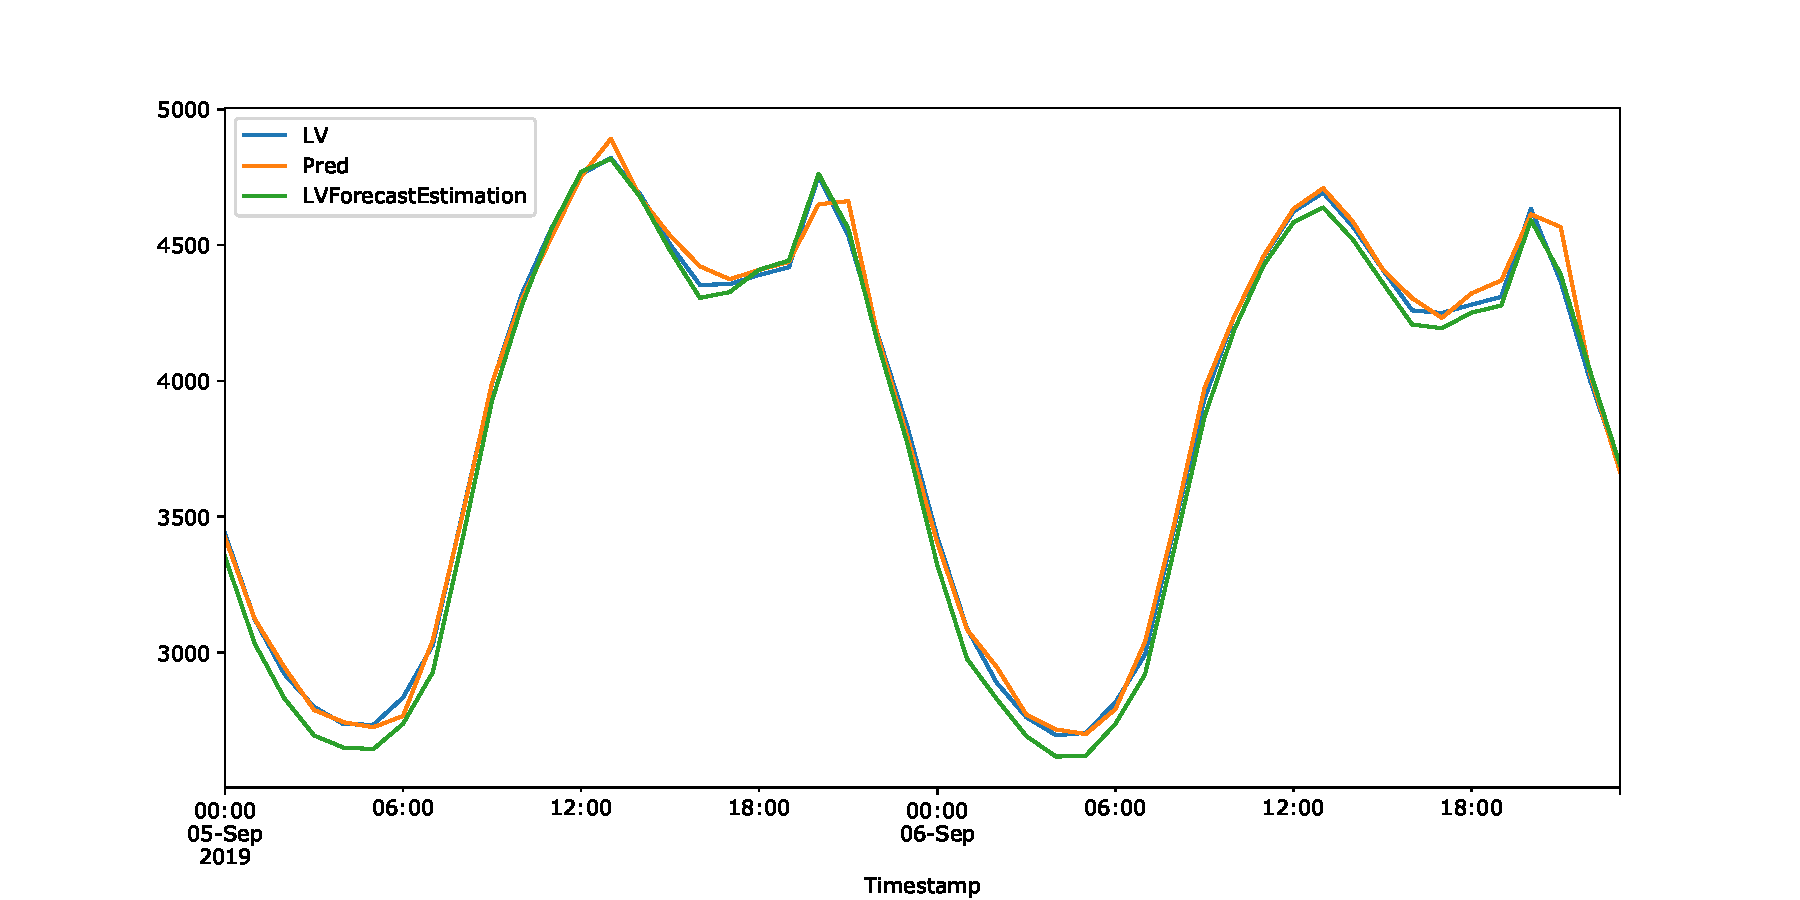
\includegraphics[width=1\linewidth]{project/last1.pdf}

\caption{LightGBM LV load forecasts vs Actual load vs OoEM’s load forecast}
\end{figure}
\begin{figure}[ht!]
\centering
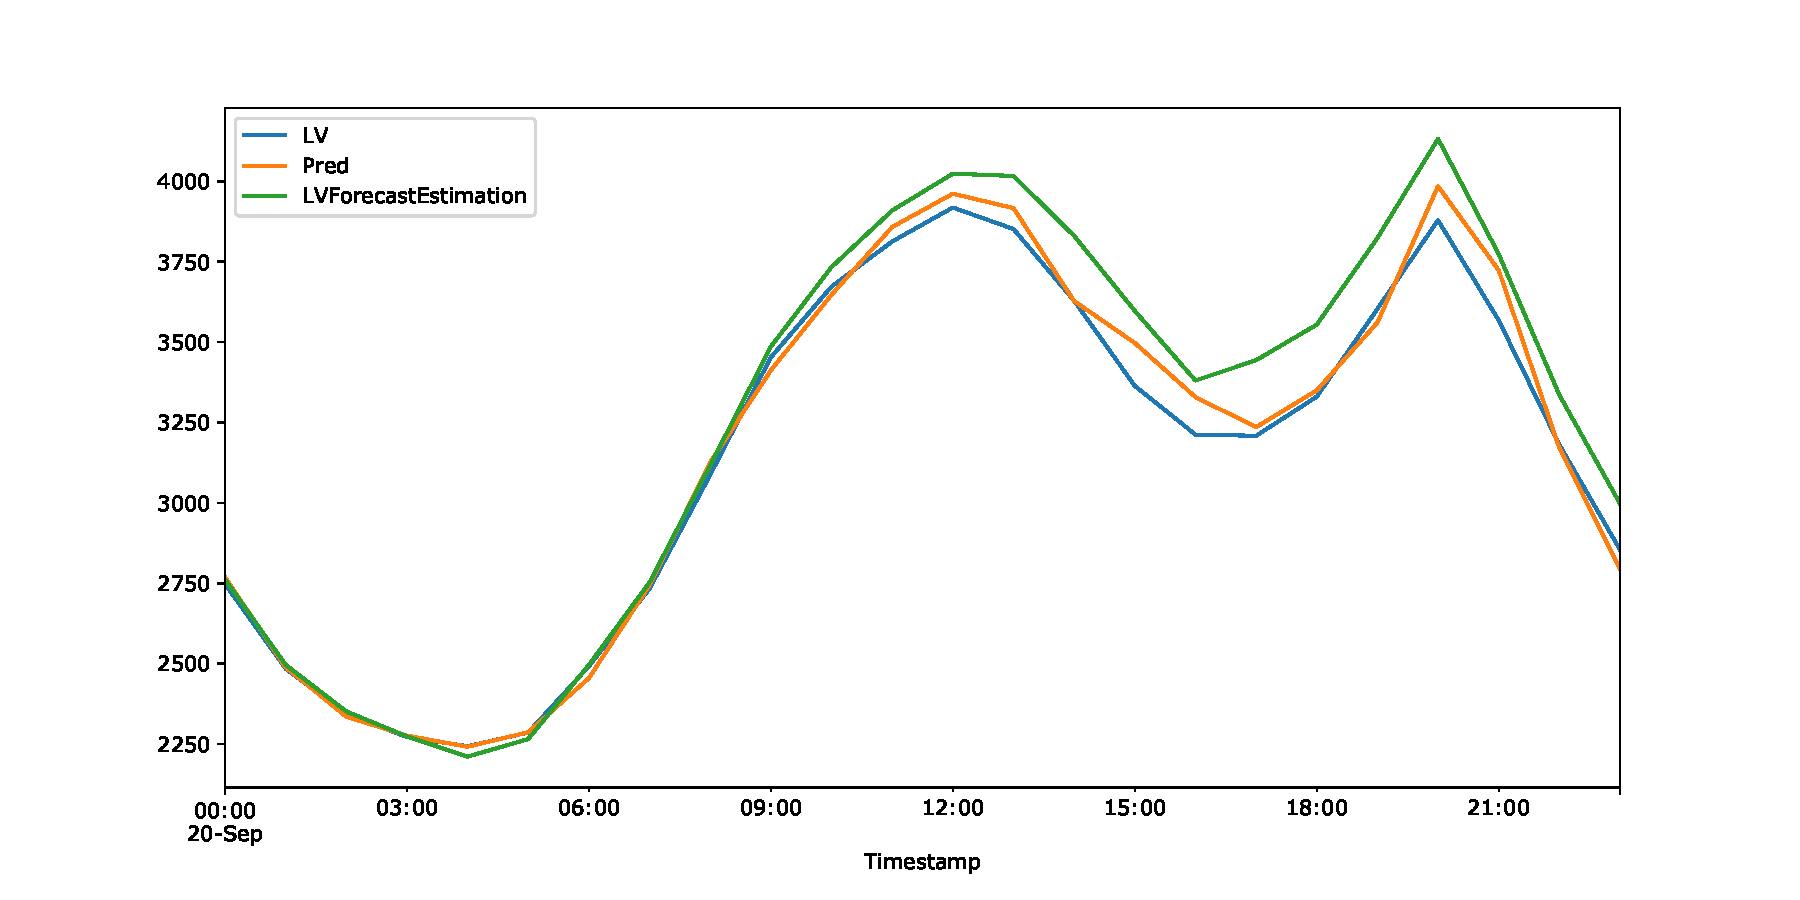
\includegraphics[width=1\linewidth]{project/last2.pdf}

\caption{LightGBM LV load forecasts vs Actual load vs OoEM’s load forecast}
\end{figure}
\begin{figure}[ht!]
\centering
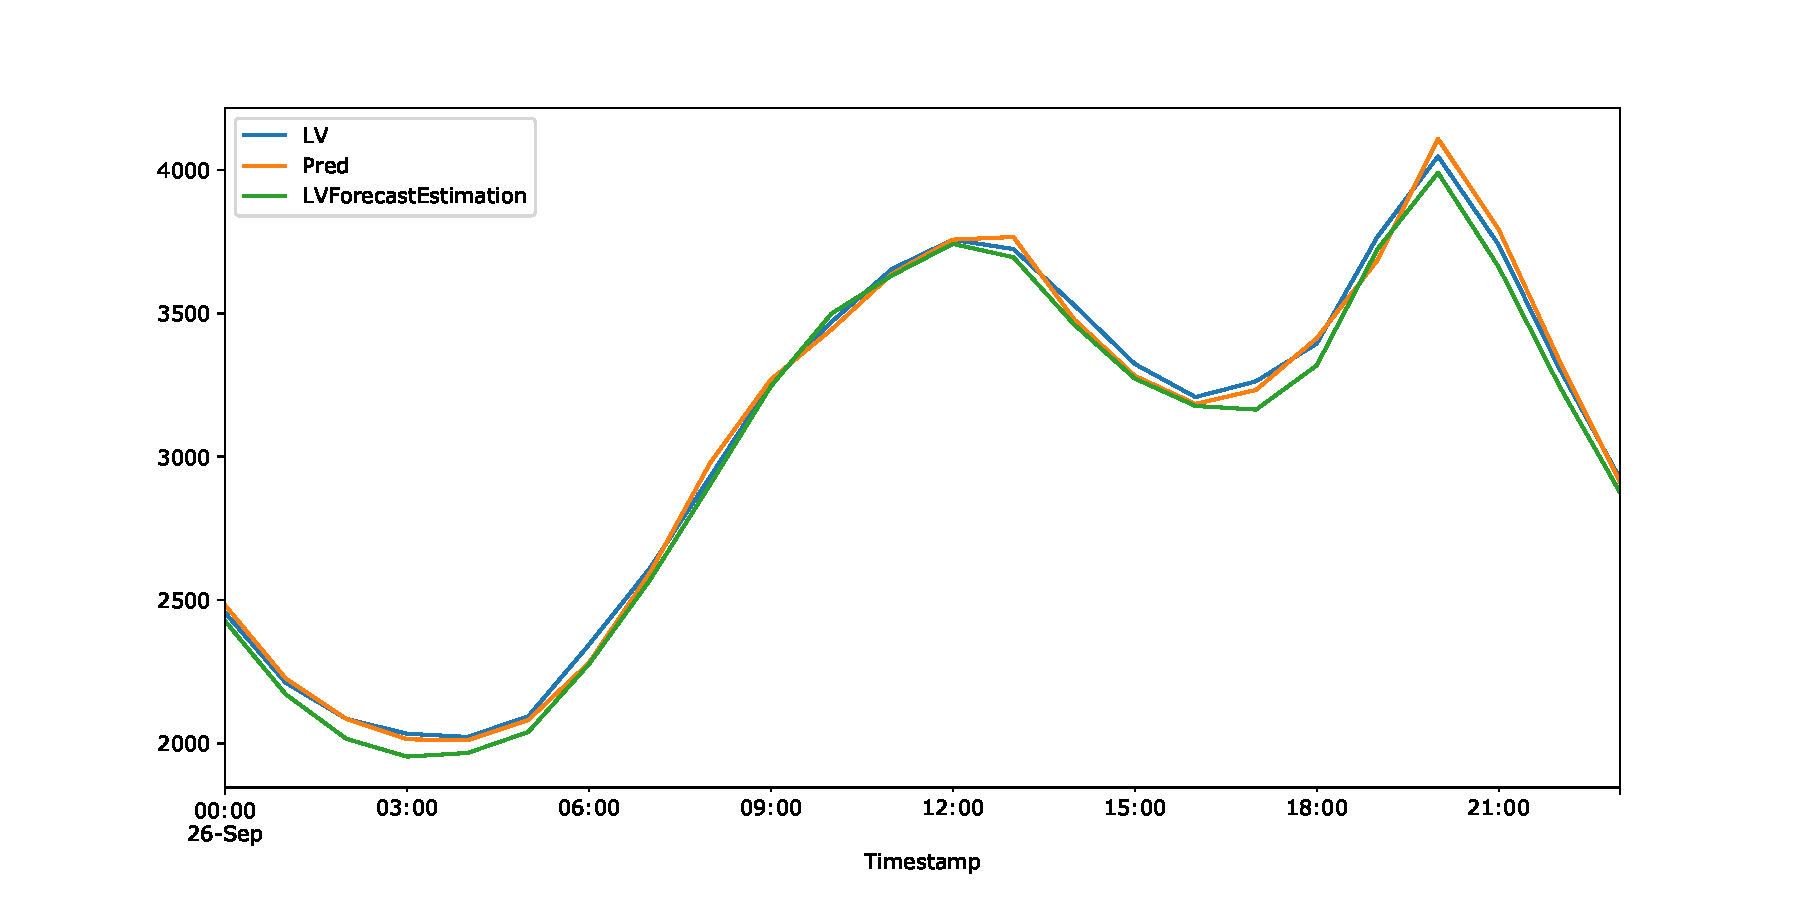
\includegraphics[width=1\linewidth]{project/last3.pdf}

\caption{LightGBM LV load forecasts vs Actual load vs OoEM’s load forecast}
\end{figure}